% -*- coding: utf-8 -*-

\documentclass[a4paper,dvipdfmx]{jsarticle}
\usepackage{ascmac,alltt,txfonts,url}

\usepackage[dvipdfmx]{graphicx}
\usepackage{here}
\usepackage{fancyvrb}

\renewcommand{\ttdefault}{cmtt}
\renewcommand{\figurename}{図} 
\renewcommand{\tablename}{表} 
\DeclareMathAlphabet{\mathtt}{OT1}{cmtt}{m}{n}
\SetMathAlphabet{\mathtt}{bold}{OT1}{cmtt}{m}{n}
\setlength{\oddsidemargin}{0cm}
\setlength{\evensidemargin}{0cm}

\makeatletter

\newdimen\@mojihaba
\settowidth{\@mojihaba}{あ}

\def\tokushu#1{%
\def\tokushutitle{#1}%
\gdef\articleHeader{\hbox to\textwidth{\rule{3\@mojihaba}{1mm}%
\hbox{\small\bf\hskip1mm \tokushutitle}\leaderfill}}
}

\newdimen \JQ	\JQ .259817mm	%%%	\JQ/\Q = 10pt/9.62216pt
\newdimen \Q	\Q  .25mm	%%%	Quarter of 1mm

\def\JarticleHeader{\rule{\textwidth}{1mm}}%
\def\JarticleTitle{{\huge\bf\@title}}
\def\JarticleAuthor{\large\begin{tabular}[t]{@{}l}\@author\end{tabular}}
\newbox\@temptitlebox

\def\verse{\let\\=\@centercr 
 \list{}{\itemsep\z@ \itemindent -1.5em\listparindent \itemindent 
 \rightmargin\leftmargin\advance\leftmargin 1.5em}\item[]}
\let\endverse\endlist
\def\quotation{\list{}{\listparindent 1.5em
 \itemindent\listparindent
 \rightmargin\leftmargin \parsep 0pt plus 1pt}\item[]}
\let\endquotation=\endlist
\def\quote{\list{}{\rightmargin\leftmargin}\item[]}
\let\endquote=\endlist
\def\abstquotation{\list{}{\listparindent 1.5em
 \itemindent\listparindent
 \leftmargin 5mm
 \rightmargin\leftmargin \parsep 0pt plus 1pt}\item[]}
\let\endabstquotation=\endlist
\def\quote{\list{}{\rightmargin\leftmargin}\item[]}
\let\endquote=\endlist

\global\def\@maketitle{\newpage \null
\hbox{\vbox to193.5\Q{\baselineskip=10mm % 193.5\Q = 9*\baselineskip
\begin{flushleft}
\JarticleHeader
% following extra vskip together with baselineskip(10mm) will produce
% appropriate 10mm/6mm gap between the rule and title
% This assumes that title is typeset with 28Q(7mm) font, and baseline
% is set 1mm above the bottom of the font.
\setbox\@temptitlebox\hbox{JarticleTitle}\ifdim\wd\@temptitlebox>\textwidth\vskip2mm\else\vskip6mm\fi
\leftskip=5mm
\JarticleTitle
\vskip6mm % to leave 10mm gap between title and author
\JarticleAuthor
\end{flushleft}\vfil}}
%\JEabstInsert
  \begin{small}
    \begin{abstquotation}
      \Jabstcontent
    \end{abstquotation}
  \end{small}
}

\long\def\Jabstract#1{\global\long\def\Jabstcontent{\noindent\ignorespaces #1}}
\def\Jabstcontent{\relax}

\makeatother

\usepackage{fancyhdr}
\pagestyle{fancy}
\lhead{VivadoHLSを使ったCベース設計に挑戦}
\rhead{}
\rhead{\thepage{}}
\cfoot{}
\renewcommand{\headrulewidth}{0.5pt}
\pagestyle{fancy}

\Jabstract{%
\\
C/C++ベースのFPGA開発をはじめるにあたって,まずはVivado HLSの使い方をFPGAで動作するビットストリームの作り方まで一通り学んでしまいましょう.
}

\begin{document}

\title{VivadoHLSを使ったCベース設計に挑戦}
\author{}
\date{2018年 3月19日~~第1.0版}
\maketitle

\section{はじめに}
この章では,とりあえずVivado HLSを使った開発ができるようになるために,ツールを一通り使ってC/C++で書いたコードからFPGAで動作するビットストリームを生成する作業までを一通り体験してみることにします.習うより慣れろ,ですね.

\section{Vivado HLSでの開発ステップ}
ポインタを使えない,多くの標準関数が使えないという制約はあるものの,基本的な制御構文のC/C++コードをHDLモジュールにすることができます.ここでは,簡単なプログラムをハードウェア化してみましょう.

\begin{figure}[H]
\begin{quote}
\begin{Verbatim}[frame=single, numbers=left, baselinestretch=0.8]

int bitcount(int a)
{
  int i;
  int s = 0;
  int tmp = a;
  for(i = 0; i < 32; i++){
    if((tmp & 0x01) == 0x01){
      s++;
    }
    tmp = tmp >> 1;
  }
  return s;
}
  \end{Verbatim}
 \end{quote}
\end{figure}

 \subsection{Vivado HLSプロジェクトの作成}

 %%
 \begin{figure}[H]
  \begin{center}
   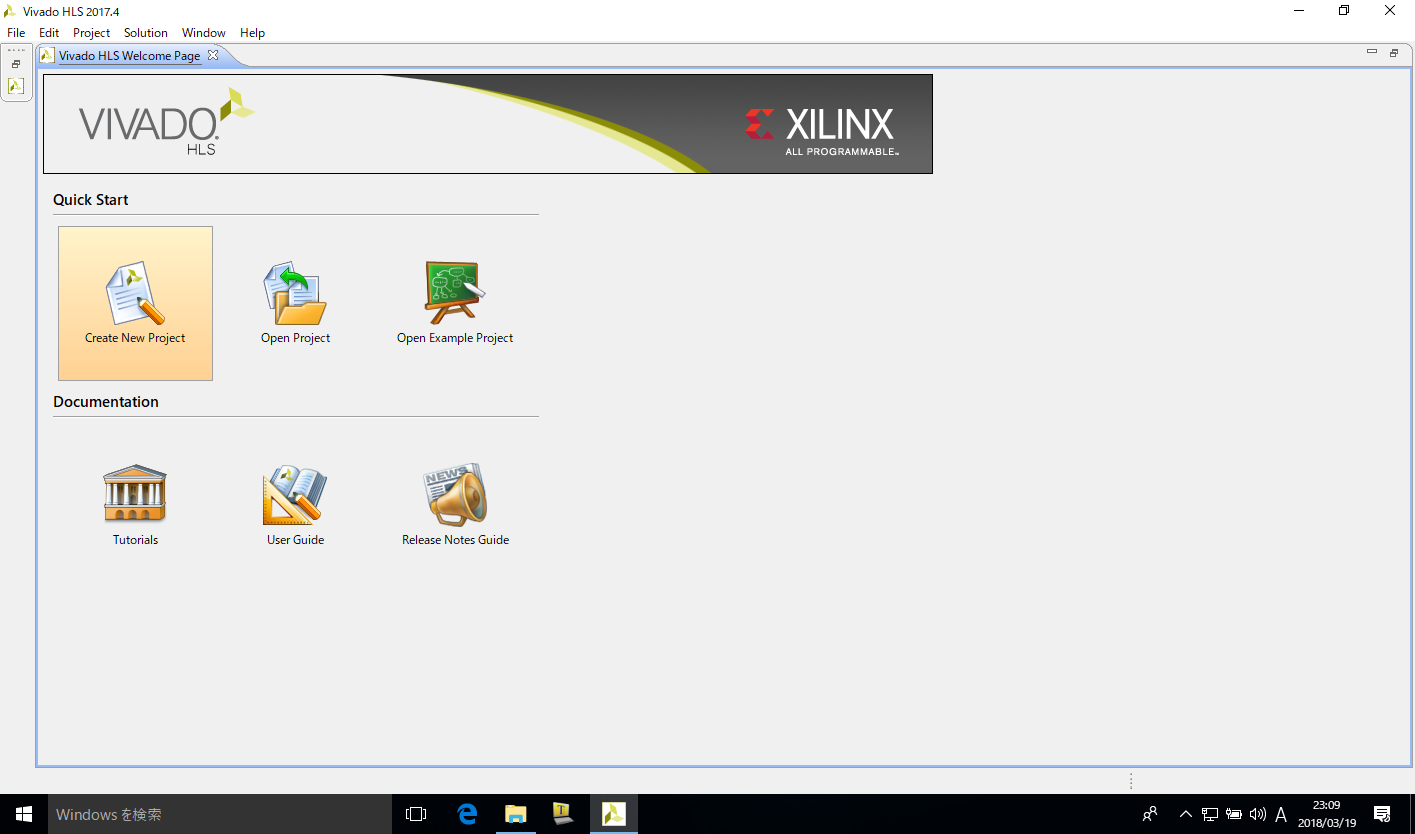
\includegraphics[width=.8\textwidth]{chapter08_figures/VirtualBox_Windows10_19_03_2018_23_09_20.png}
  \end{center}
  \caption{Vivado HLSを起動したところ.Vivado HLSはデスクトップのショートカットアイコンやスタートメニューから起動する.}
 \end{figure}

 \begin{figure}[H]
  \begin{center}
   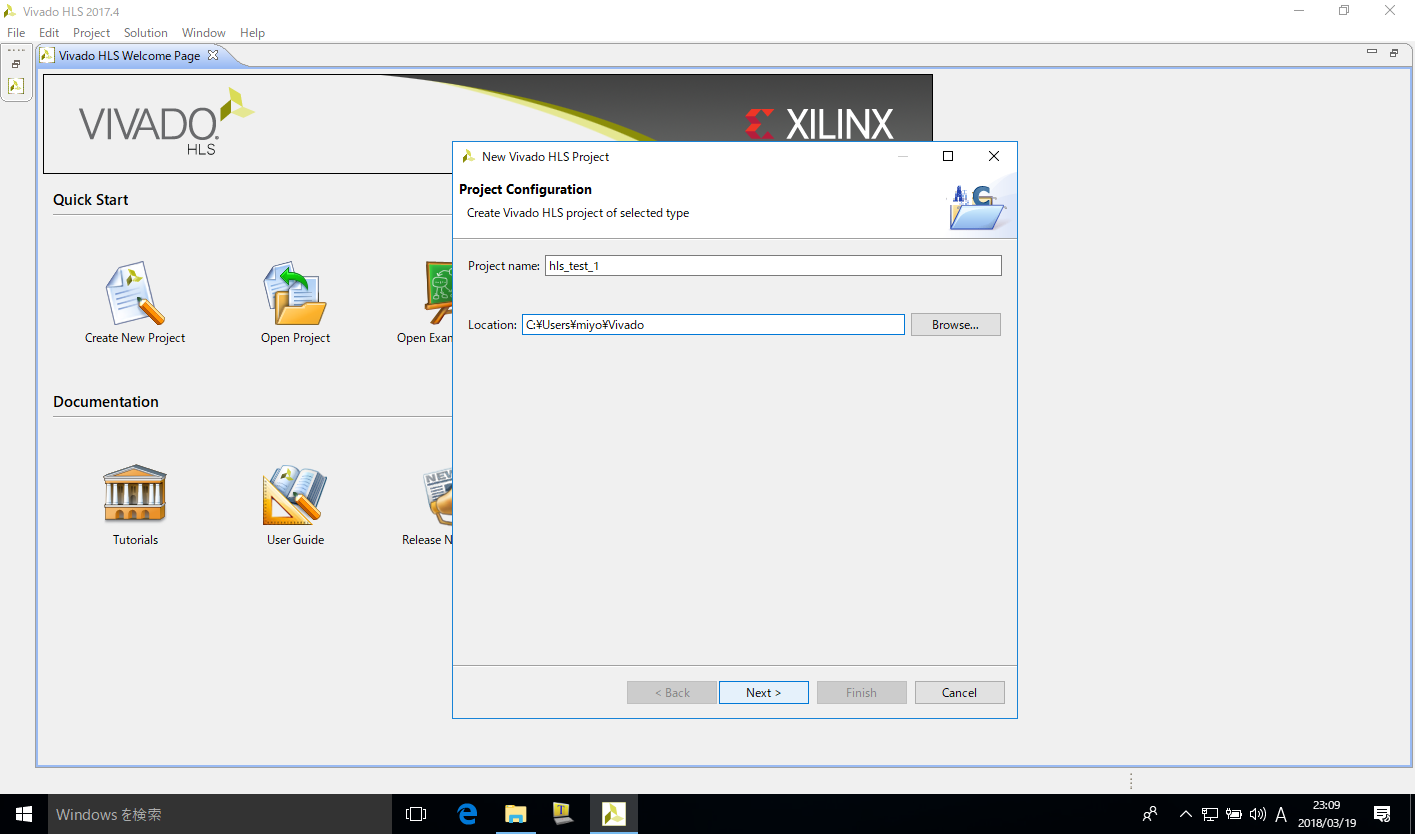
\includegraphics[width=.8\textwidth]{chapter08_figures/VirtualBox_Windows10_19_03_2018_23_10_00.png}
  \end{center}
  \caption{プロジェクト名と格納フォルダを指定.ここでは.ホームの下のVivadoの下に格納することとし,名前をhls\_test\_1とした}
 \end{figure}

 \begin{figure}[H]
  \begin{center}
   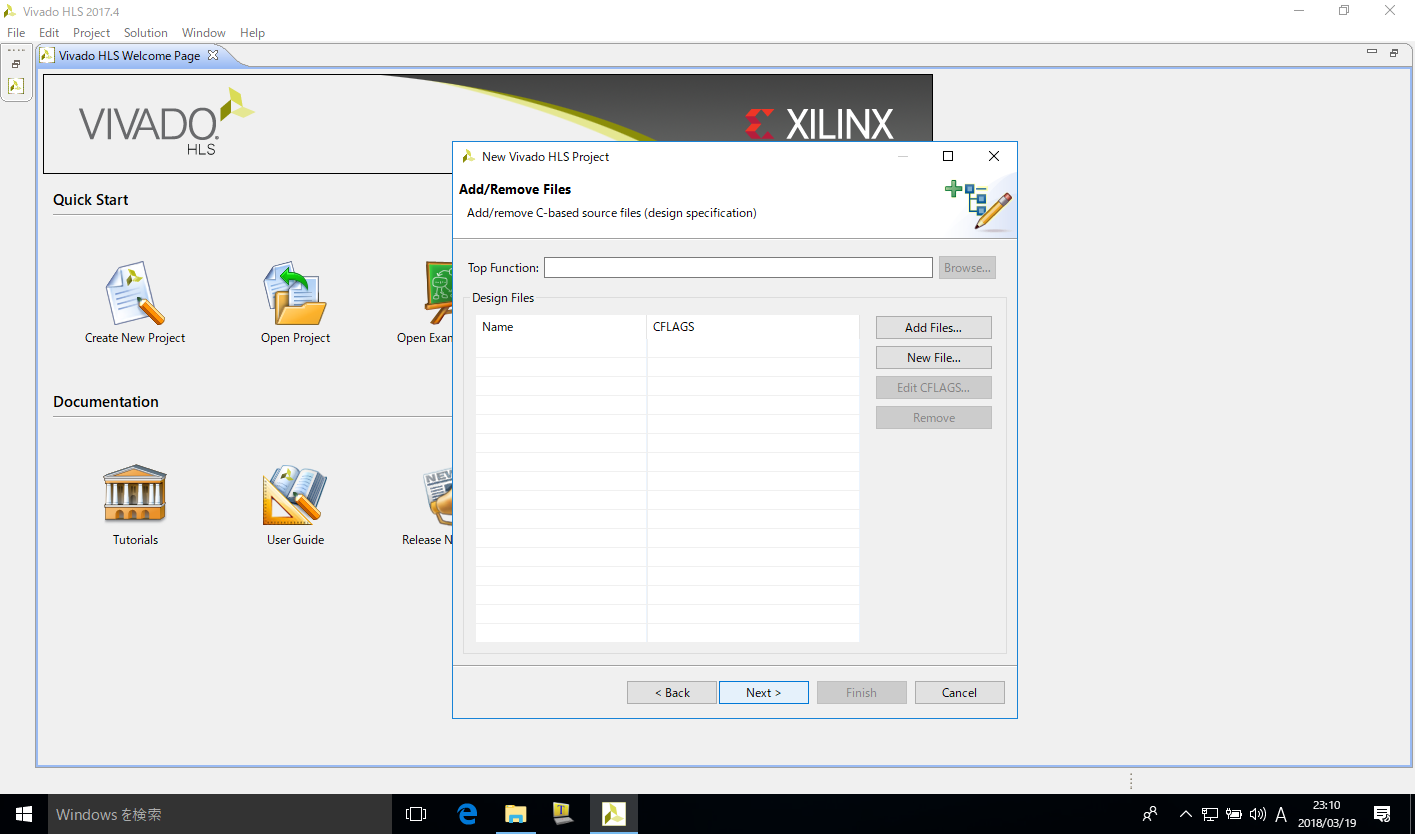
\includegraphics[width=.8\textwidth]{chapter08_figures/VirtualBox_Windows10_19_03_2018_23_10_06.png}
  \end{center}
  \caption{既存の設計ソースコードがあれば,ここで追加.ないのでNextで次へ.}
 \end{figure}

 \begin{figure}[H]
  \begin{center}
   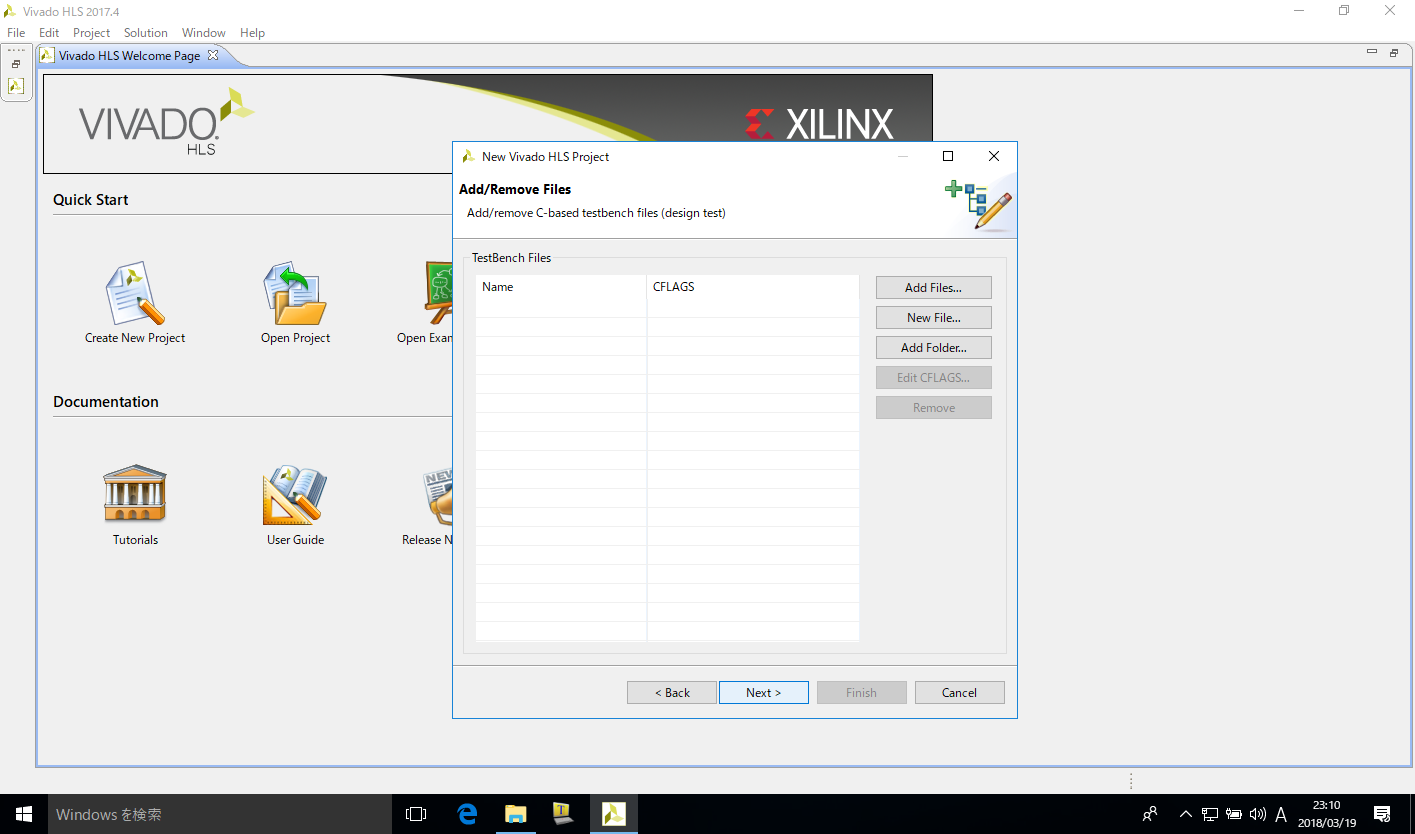
\includegraphics[width=.8\textwidth]{chapter08_figures/VirtualBox_Windows10_19_03_2018_23_10_10.png}
  \end{center}
  \caption{既存のテストベンチ用のソースコードがあれば,ここで追加.ないのでNextで次へ.}
 \end{figure}

 \begin{figure}[H]
  \begin{center}
   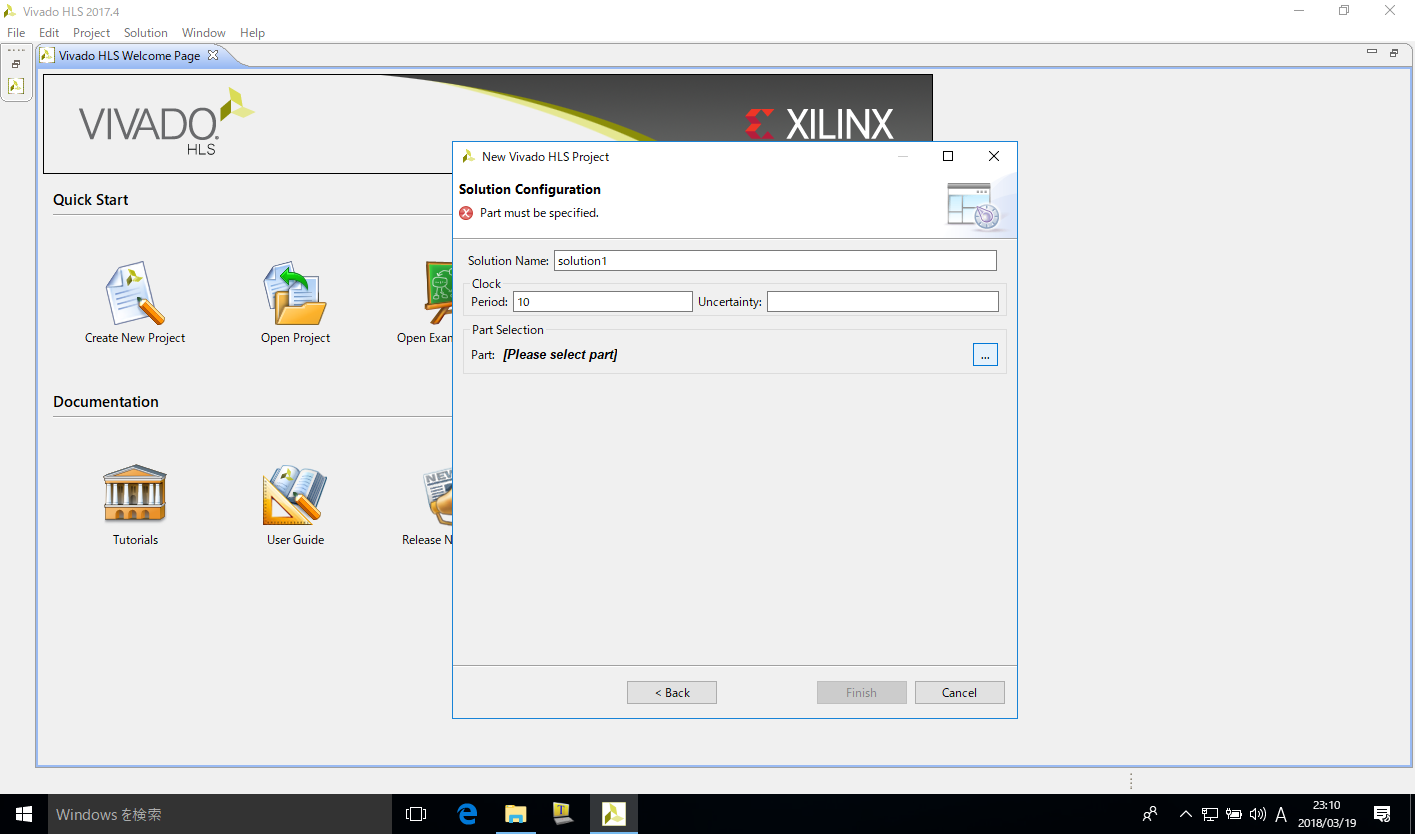
\includegraphics[width=.8\textwidth]{chapter08_figures/VirtualBox_Windows10_19_03_2018_23_10_19.png}
  \end{center}
  \caption{ターゲットFPGAを選択する.Part Selectionの中の...ボタンをクリック}
 \end{figure}

 \begin{figure}[H]
  \begin{center}
   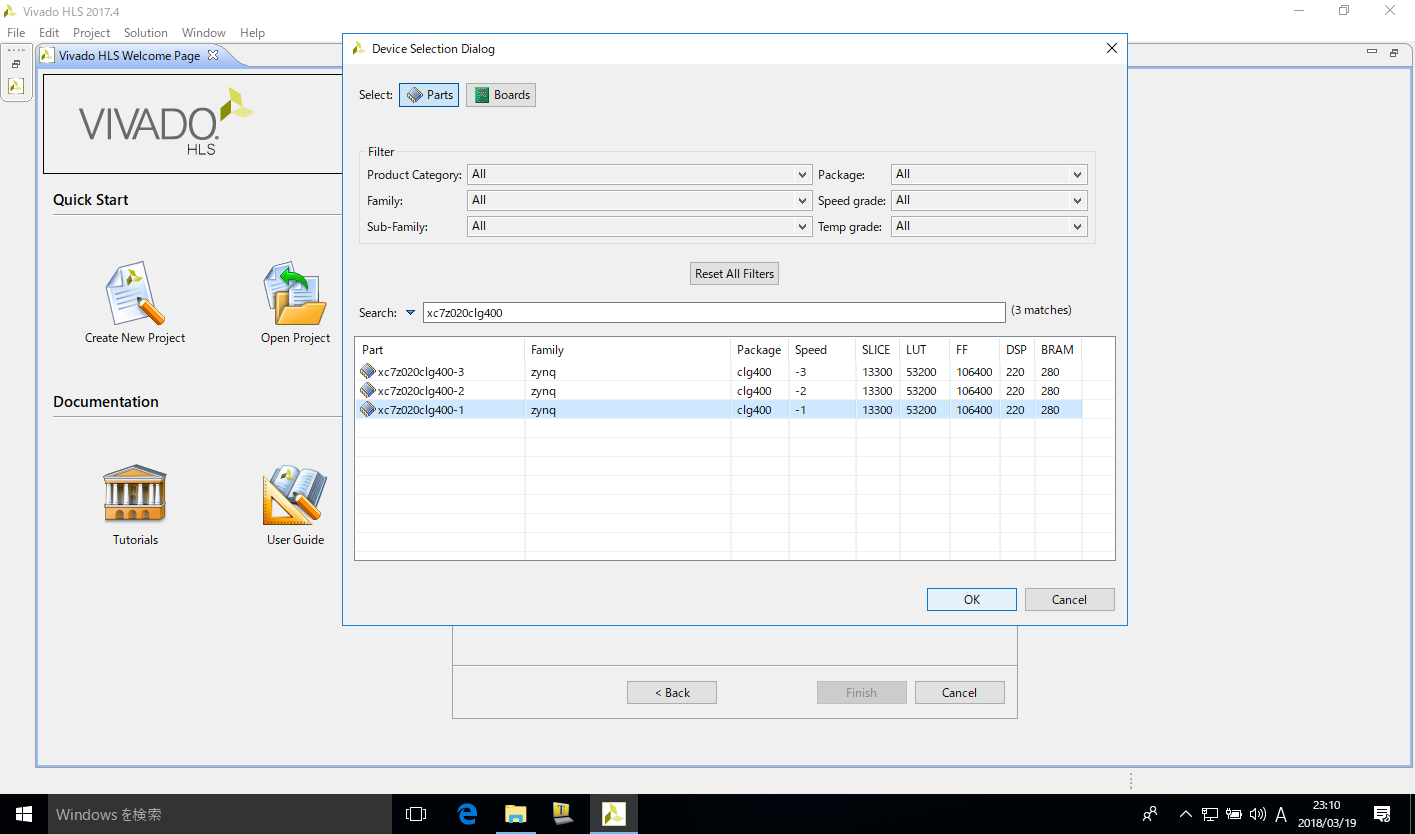
\includegraphics[width=.8\textwidth]{chapter08_figures/VirtualBox_Windows10_19_03_2018_23_10_34.png}
  \end{center}
  \caption{FPGAの型番を選択.xc7z020clg400-1を選択する.検索フィールドにxc7z020と入力していくと楽に探せる.}
 \end{figure}

 \begin{figure}[H]
  \begin{center}
   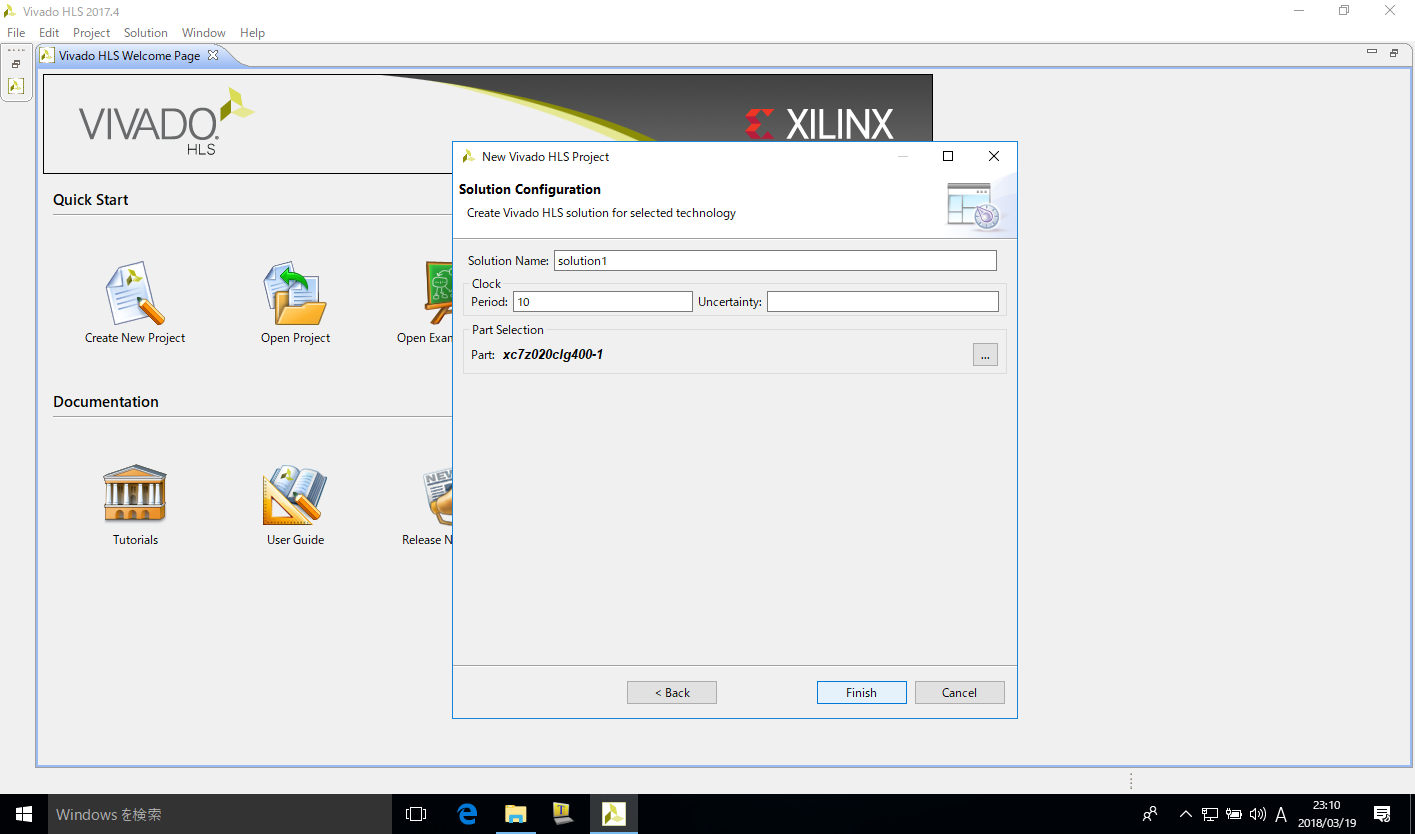
\includegraphics[width=.8\textwidth]{chapter08_figures/VirtualBox_Windows10_19_03_2018_23_10_39.png}
  \end{center}
  \caption{FPGAを選択し終えたらFinish.}
 \end{figure}

 \begin{figure}[H]
  \begin{center}
   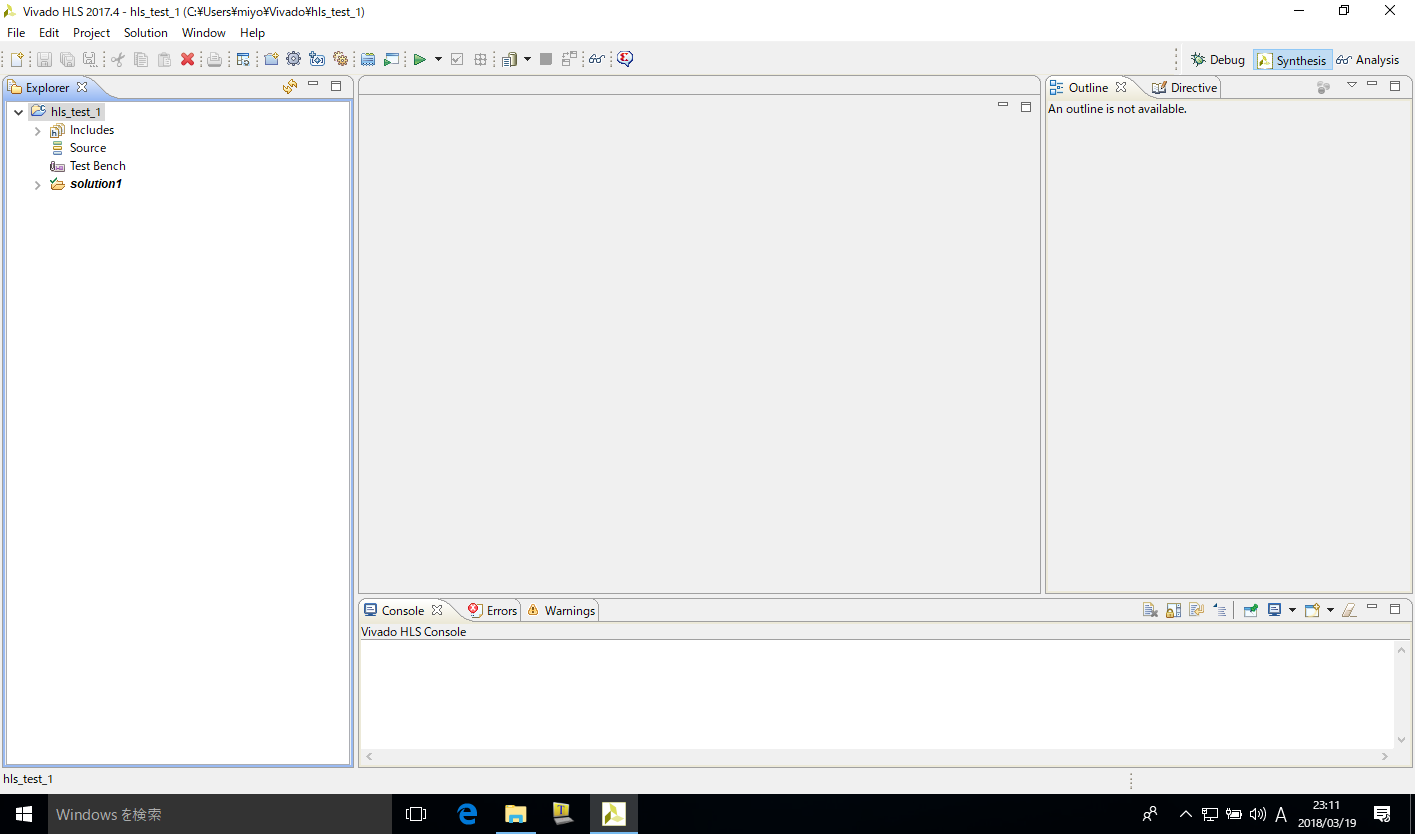
\includegraphics[width=.8\textwidth]{chapter08_figures/VirtualBox_Windows10_19_03_2018_23_11_08.png}
  \end{center}
  \caption{プロジェクトの作成が完了した}
 \end{figure}

 \subsection{Vivado HLS上での設計}

 \begin{figure}[H]
  \begin{center}
   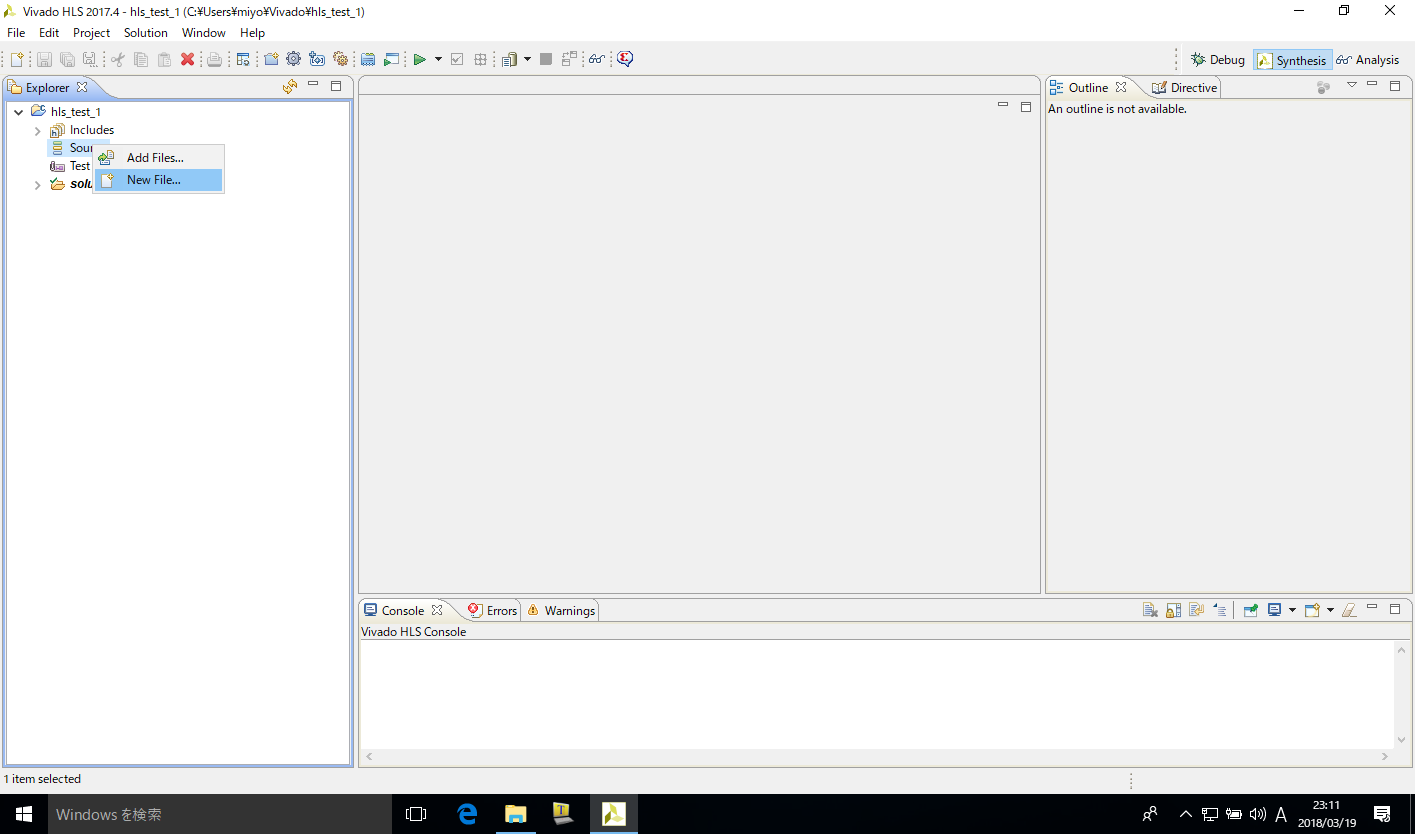
\includegraphics[width=.8\textwidth]{chapter08_figures/VirtualBox_Windows10_19_03_2018_23_11_14.png}
  \end{center}
  \caption{左ペインのSourcesアイコンの上で右クリック,New File...をクリック}
 \end{figure}

 \begin{figure}[H]
  \begin{center}
   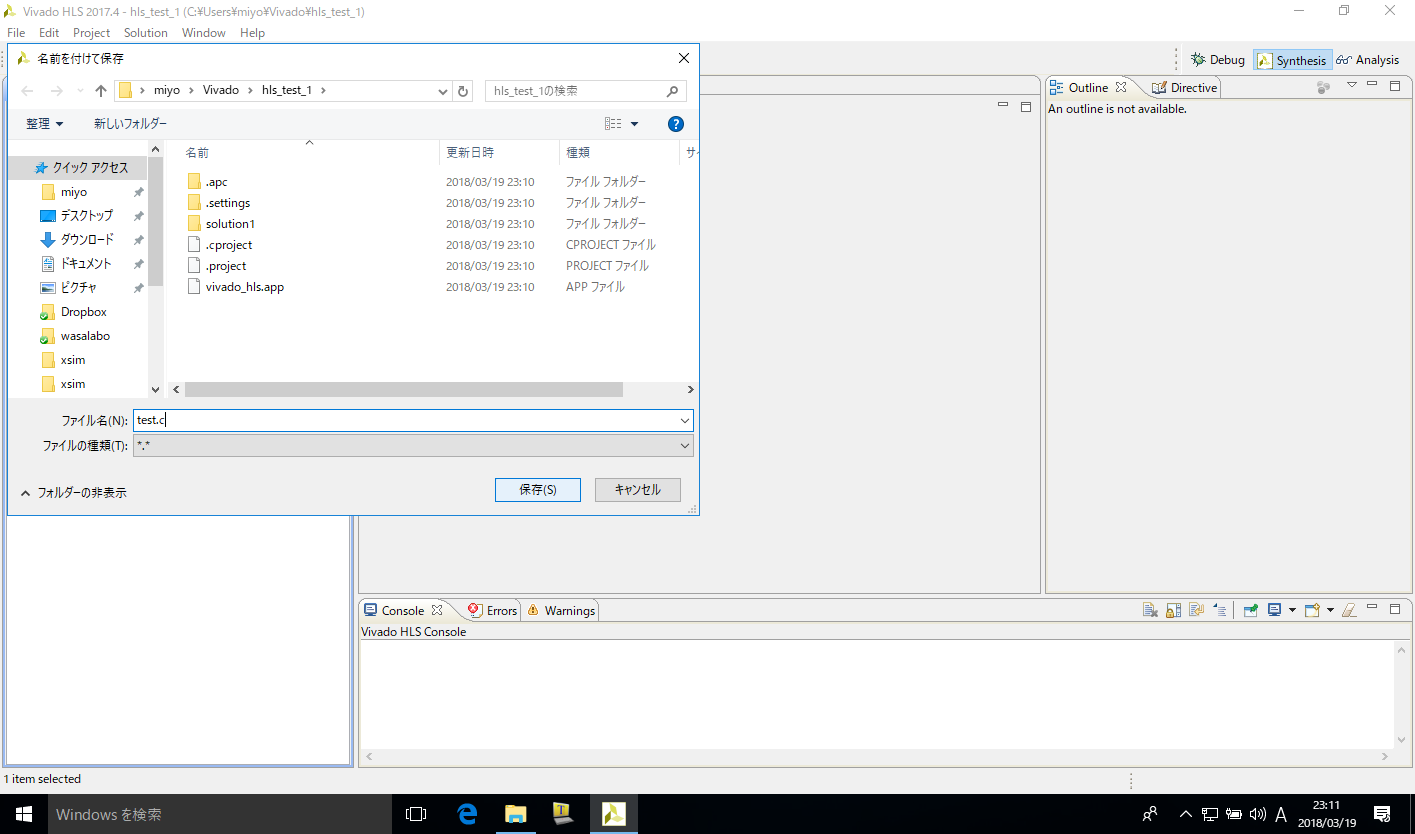
\includegraphics[width=.8\textwidth]{chapter08_figures/VirtualBox_Windows10_19_03_2018_23_11_22.png}
  \end{center}
  \caption{開いたファイル選択ダイアログに,作成するファイル test.c と入力して保存をクリック}
 \end{figure}

 %%
 \begin{figure}[H]
  \begin{center}
   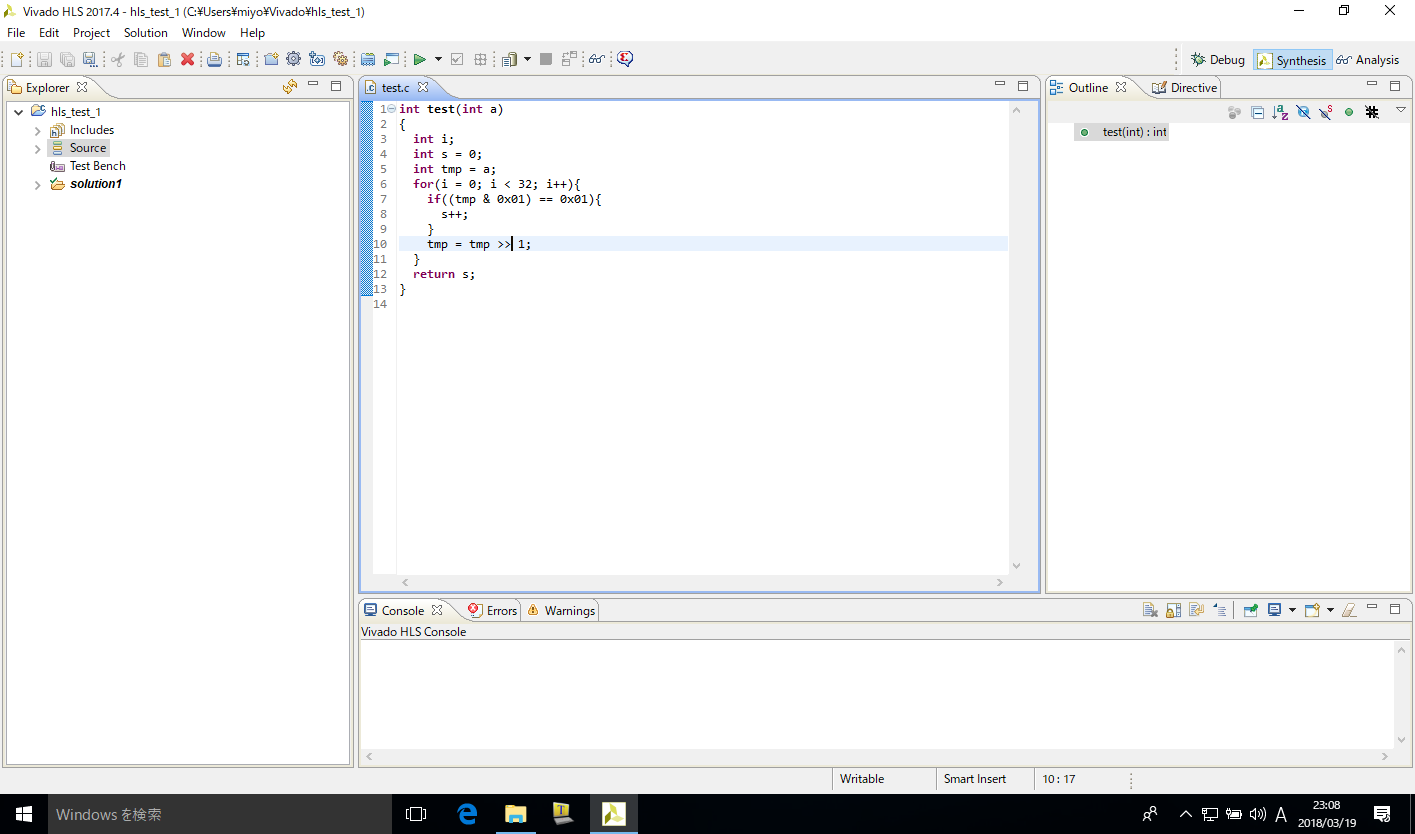
\includegraphics[width=.8\textwidth]{chapter08_figures/VirtualBox_Windows10_19_03_2018_23_13_38.png}
  \end{center}
  \caption{作成したtest.cの中身として,先のソースコードを入力する.}
 \end{figure}

 \begin{figure}[H]
  \begin{center}
   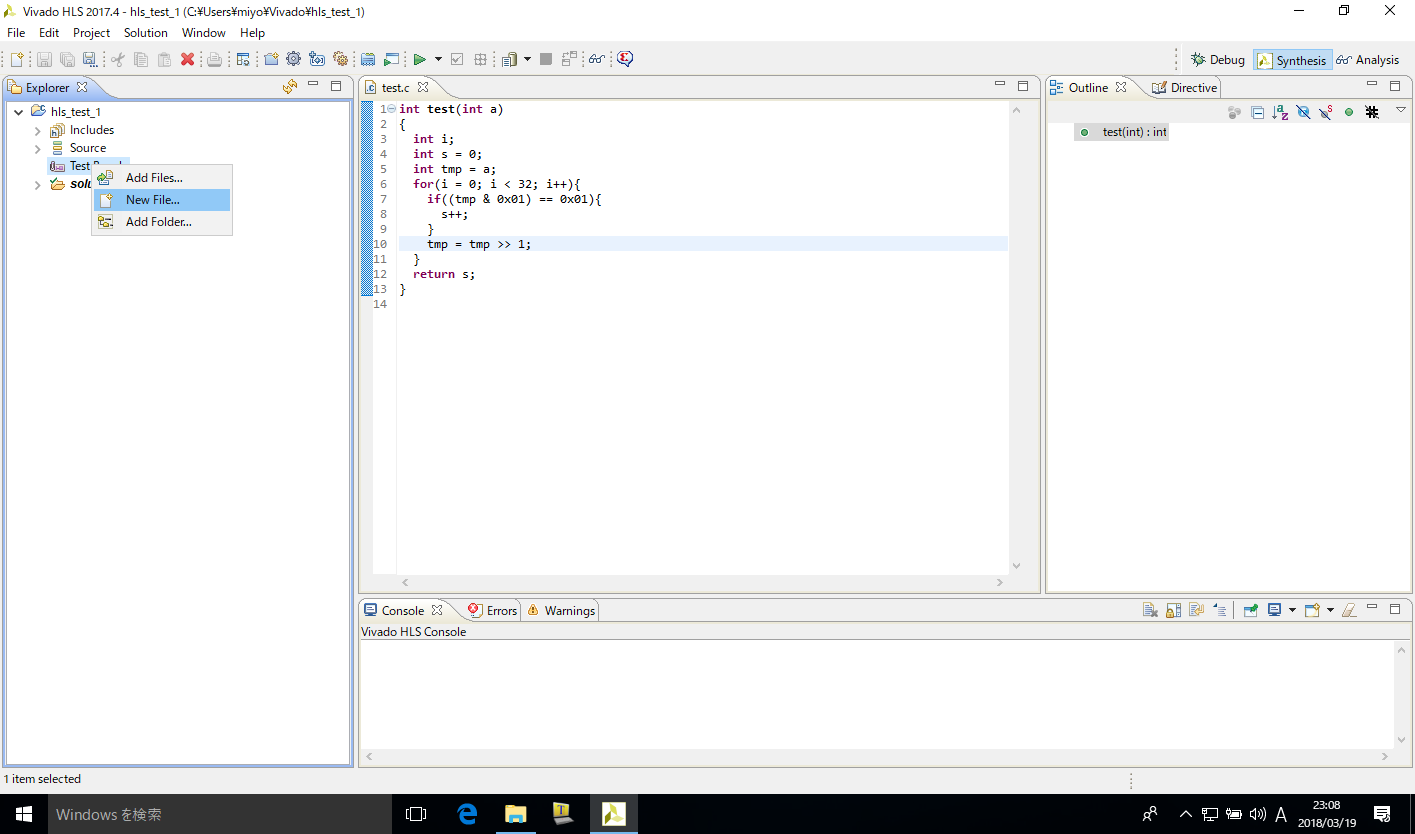
\includegraphics[width=.8\textwidth]{chapter08_figures/VirtualBox_Windows10_19_03_2018_23_13_47.png}
  \end{center}
  \caption{動作確認のために,テストベンチ用のソースコードを追加する.今度はTest Benchアイコンの上で右クリック,New File...をクリック }
 \end{figure}

 \begin{figure}[H]
  \begin{center}
   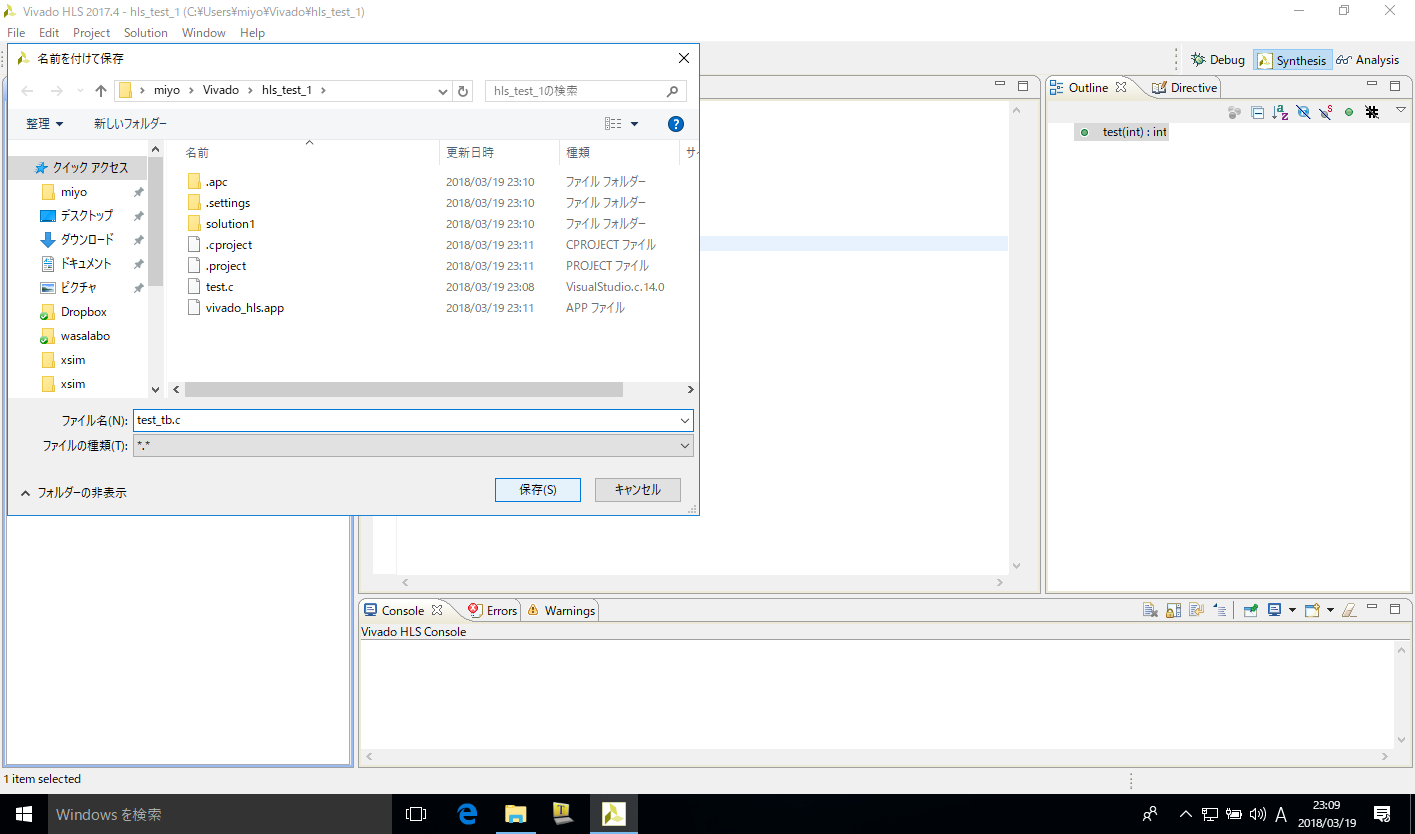
\includegraphics[width=.8\textwidth]{chapter08_figures/VirtualBox_Windows10_19_03_2018_23_14_03.png}
  \end{center}
  \caption{今度はtest\_tb.cというファイルを作成することにする.ファイル名を入力して保存をクリック}
 \end{figure}

 \begin{figure}[H]
  \begin{center}
   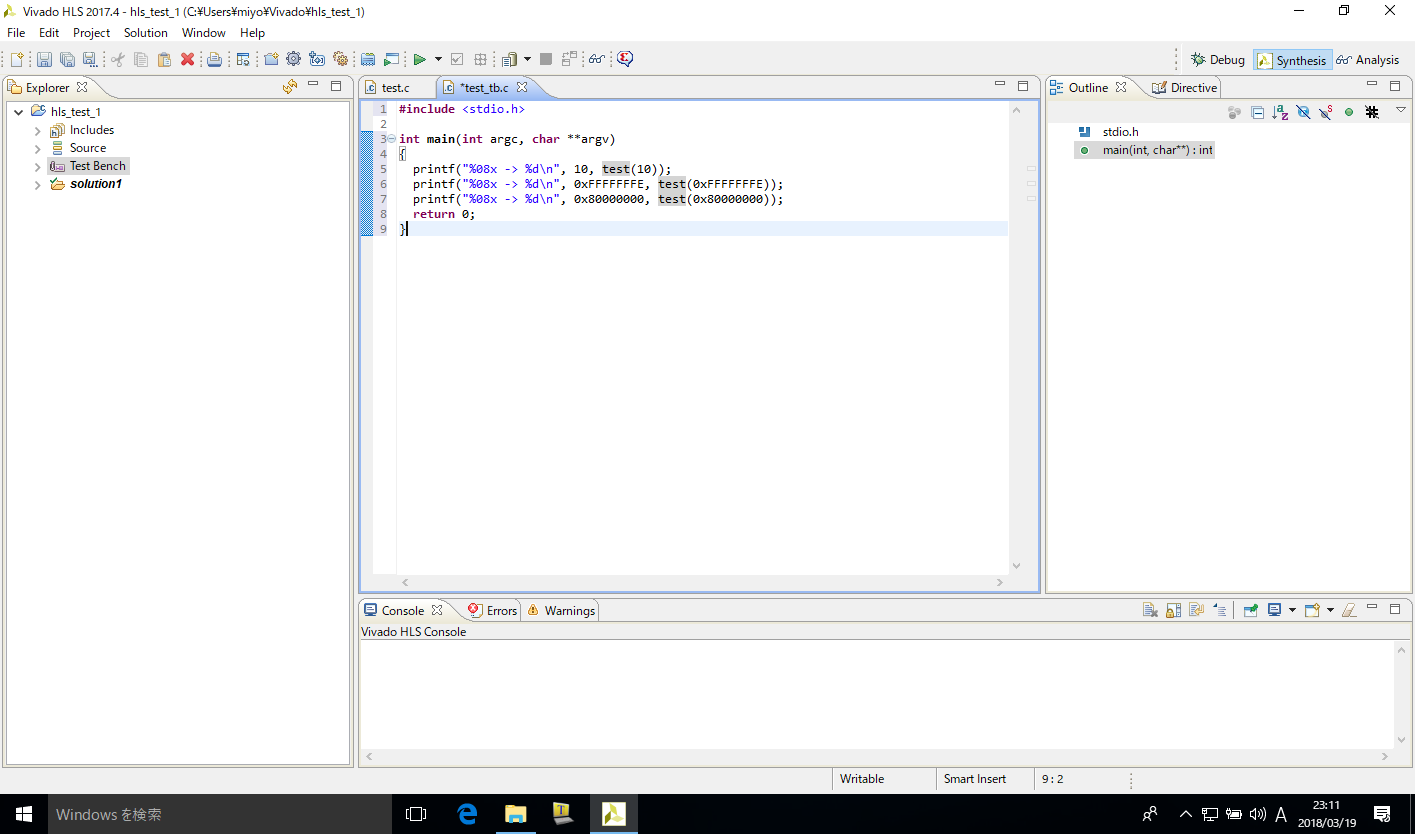
\includegraphics[width=.8\textwidth]{chapter08_figures/VirtualBox_Windows10_19_03_2018_23_15_37.png}
  \end{center}
  \caption{テストベンチの中身を記述する.テストベンチは単なるCプログラムなのでstdio.hやprintf関数が使える}
 \end{figure}

 \begin{figure}[H]
  \begin{center}
   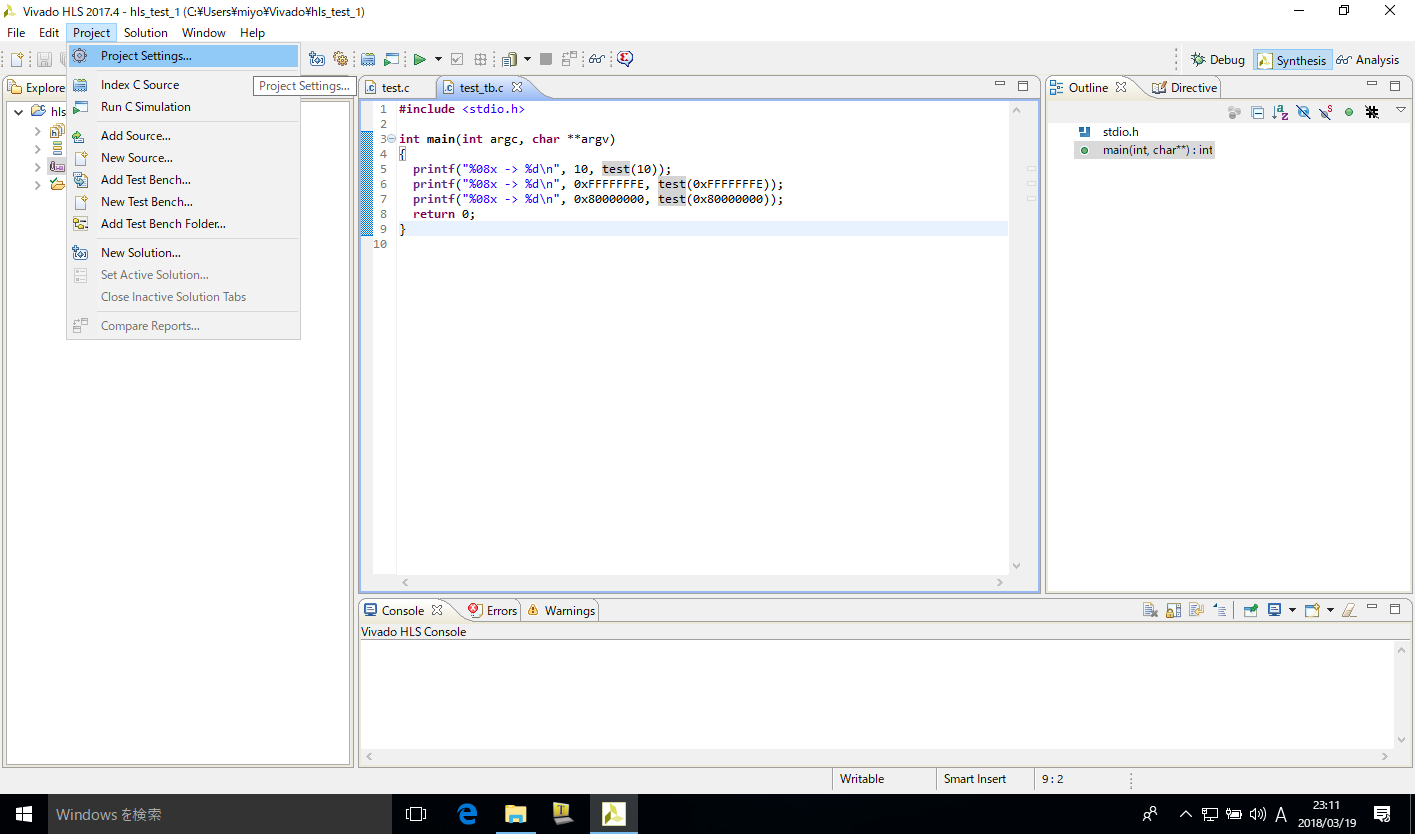
\includegraphics[width=.8\textwidth]{chapter08_figures/VirtualBox_Windows10_19_03_2018_23_15_45.png}
  \end{center}
  \caption{メニューのProjectからProject Settings...をクリックして,プロジェクトの設定をする}
 \end{figure}

 \begin{figure}[H]
  \begin{center}
   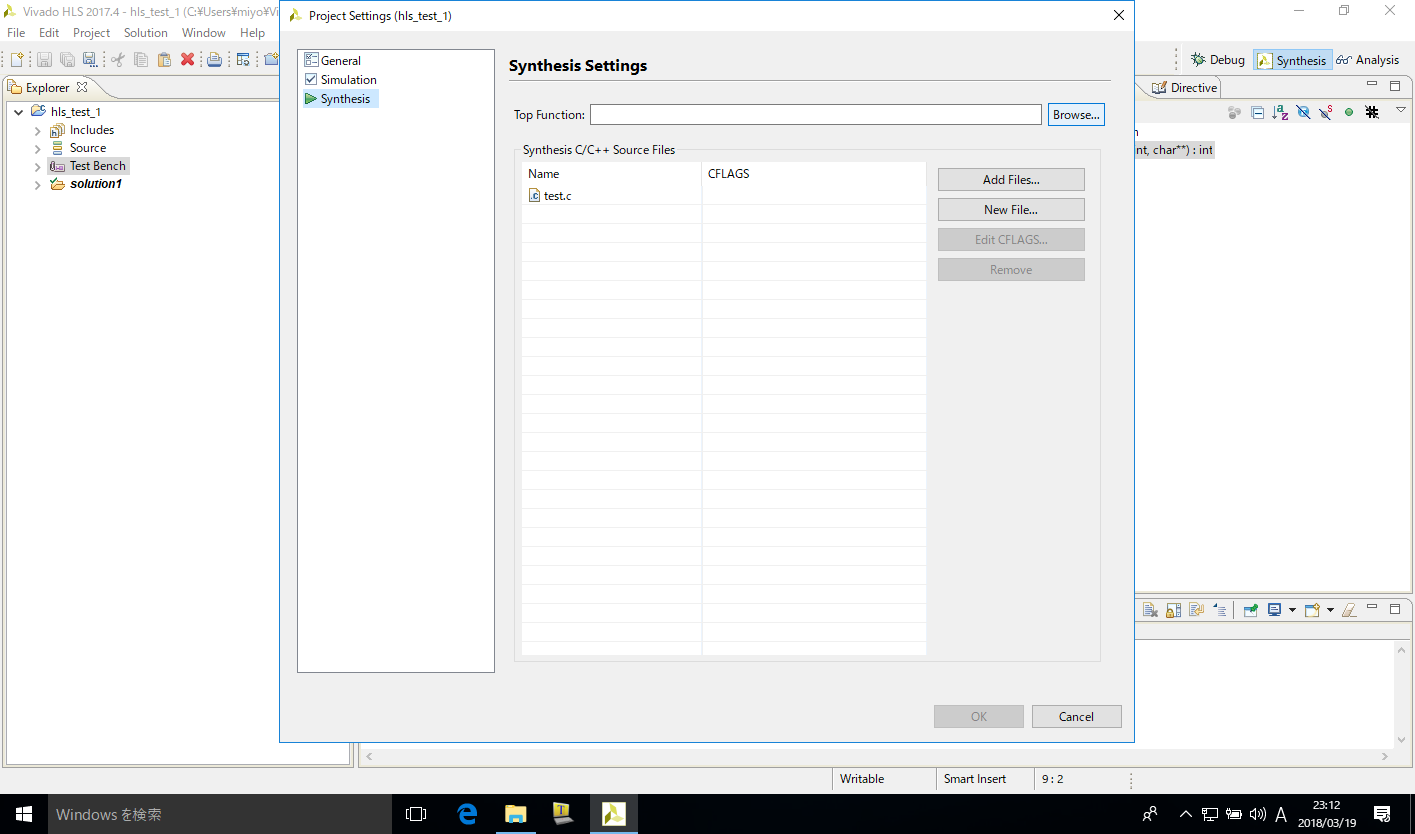
\includegraphics[width=.8\textwidth]{chapter08_figures/VirtualBox_Windows10_19_03_2018_23_15_58.png}
  \end{center}
  \caption{Synthesisをみると,Top Functionが指定されていないことが確認できる}
 \end{figure}

 \begin{figure}[H]
  \begin{center}
   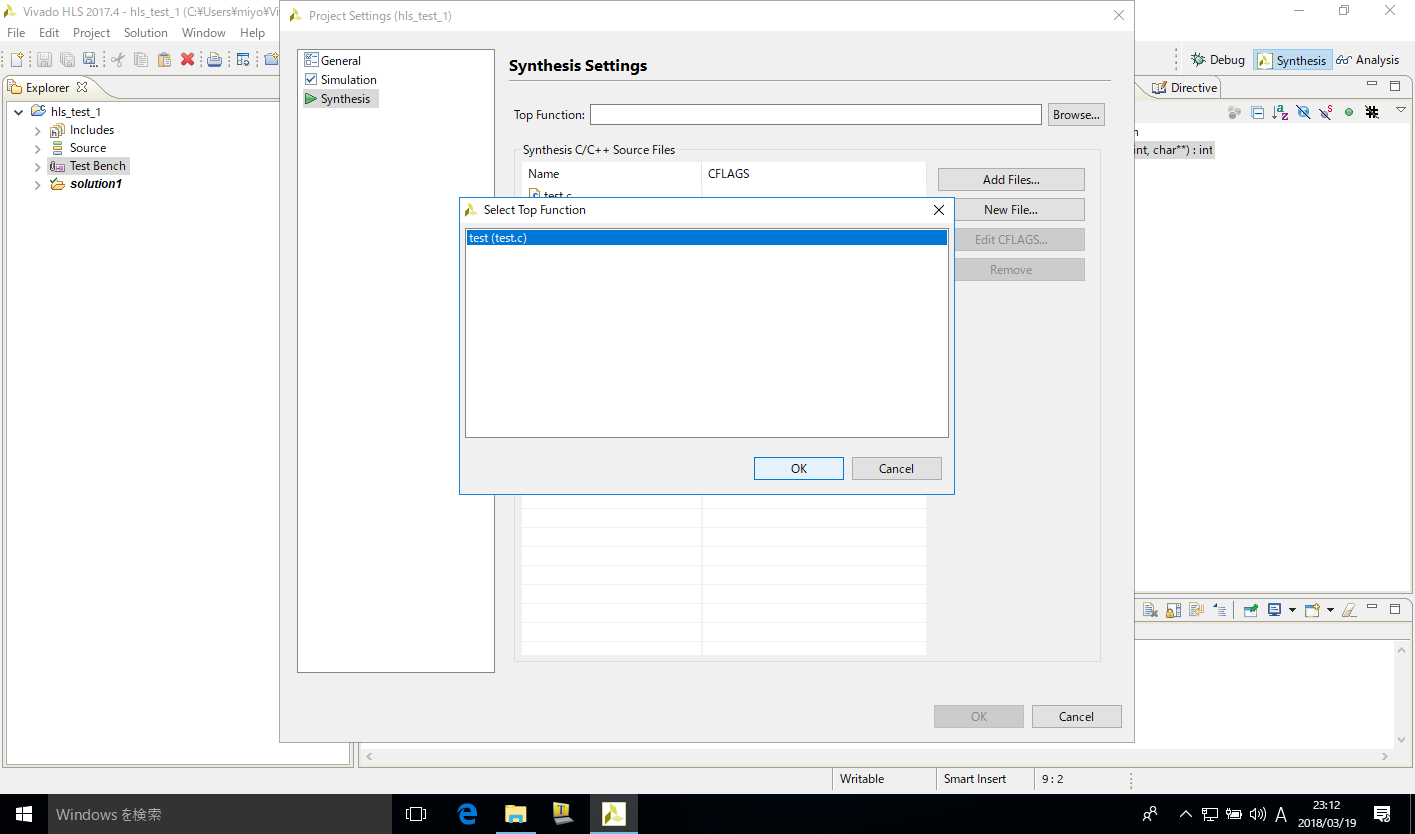
\includegraphics[width=.8\textwidth]{chapter08_figures/VirtualBox_Windows10_19_03_2018_23_16_05.png}
  \end{center}
  \caption{Browse...ボタンをクリックすると候補がでる.今回は一つだけ.候補に表示されたtest関数を選択してOKをクリック}
 \end{figure}

 \begin{figure}[H]
  \begin{center}
   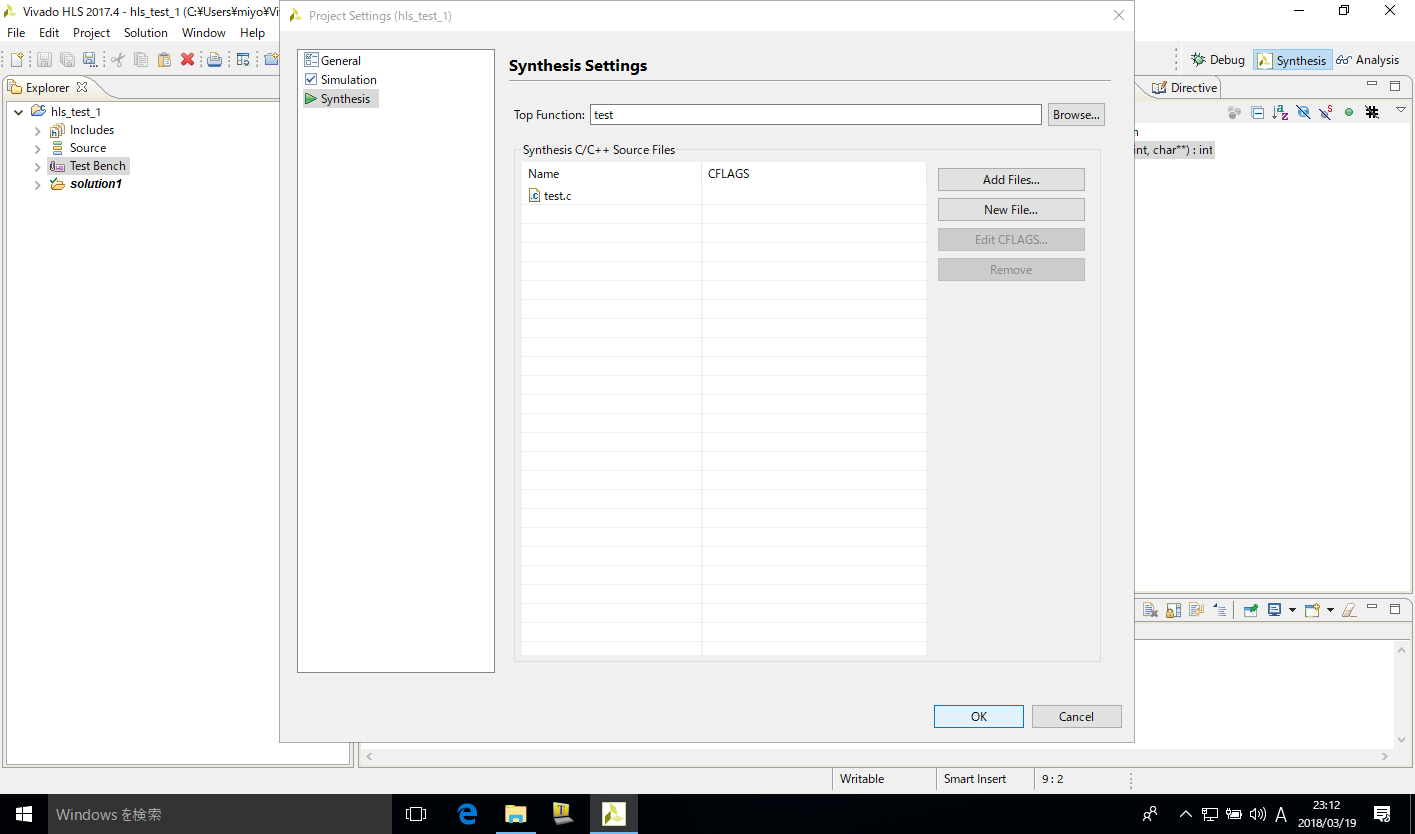
\includegraphics[width=.8\textwidth]{chapter08_figures/VirtualBox_Windows10_19_03_2018_23_16_10.png}
  \end{center}
  \caption{合成するトップの関数がtestであることを指定できた}
 \end{figure}

 \subsection{Vivado HLSでの動作確認}

 \begin{figure}[H]
  \begin{center}
   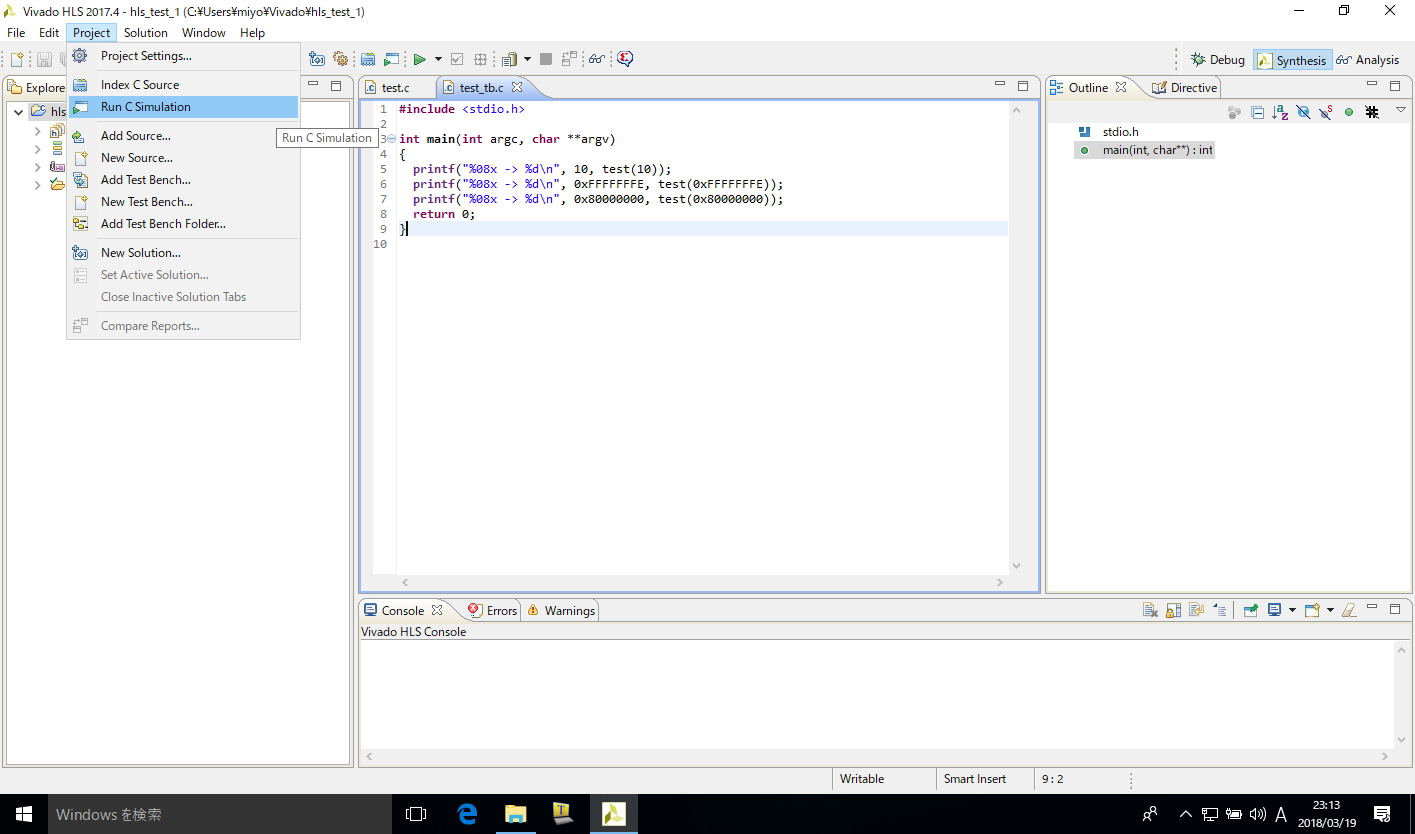
\includegraphics[width=.8\textwidth]{chapter08_figures/VirtualBox_Windows10_19_03_2018_23_16_35.png}
  \end{center}
  \caption{まずはCレベルでの動作を確認するため,メニューのProjectからRun C Simulationをクリックする}
 \end{figure}

 \begin{figure}[H]
  \begin{center}
   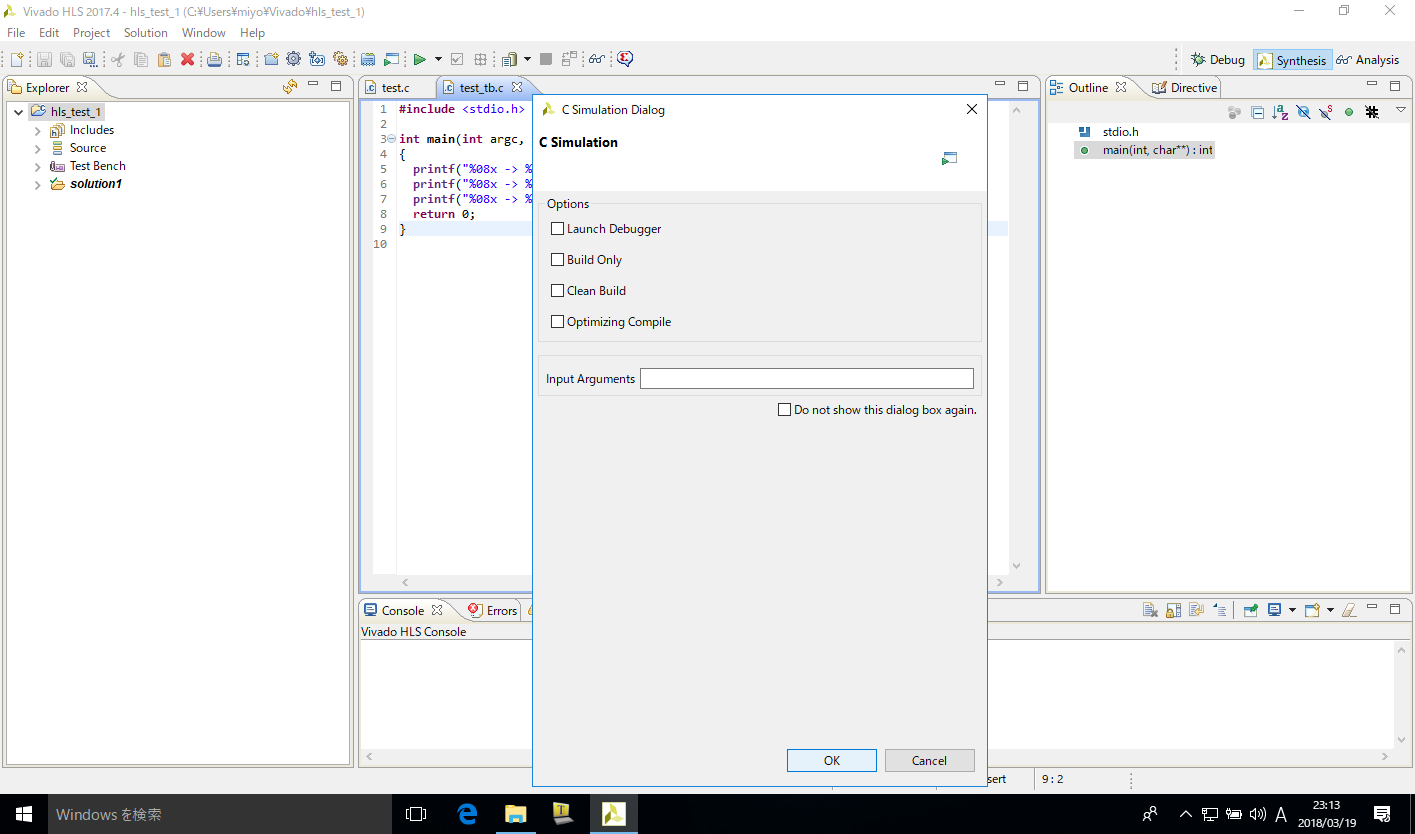
\includegraphics[width=.8\textwidth]{chapter08_figures/VirtualBox_Windows10_19_03_2018_23_16_40.png}
  \end{center}
  \caption{特にオプションは指定せずにOKをクリック}
 \end{figure}

 %%
 \begin{figure}[H]
  \begin{center}
   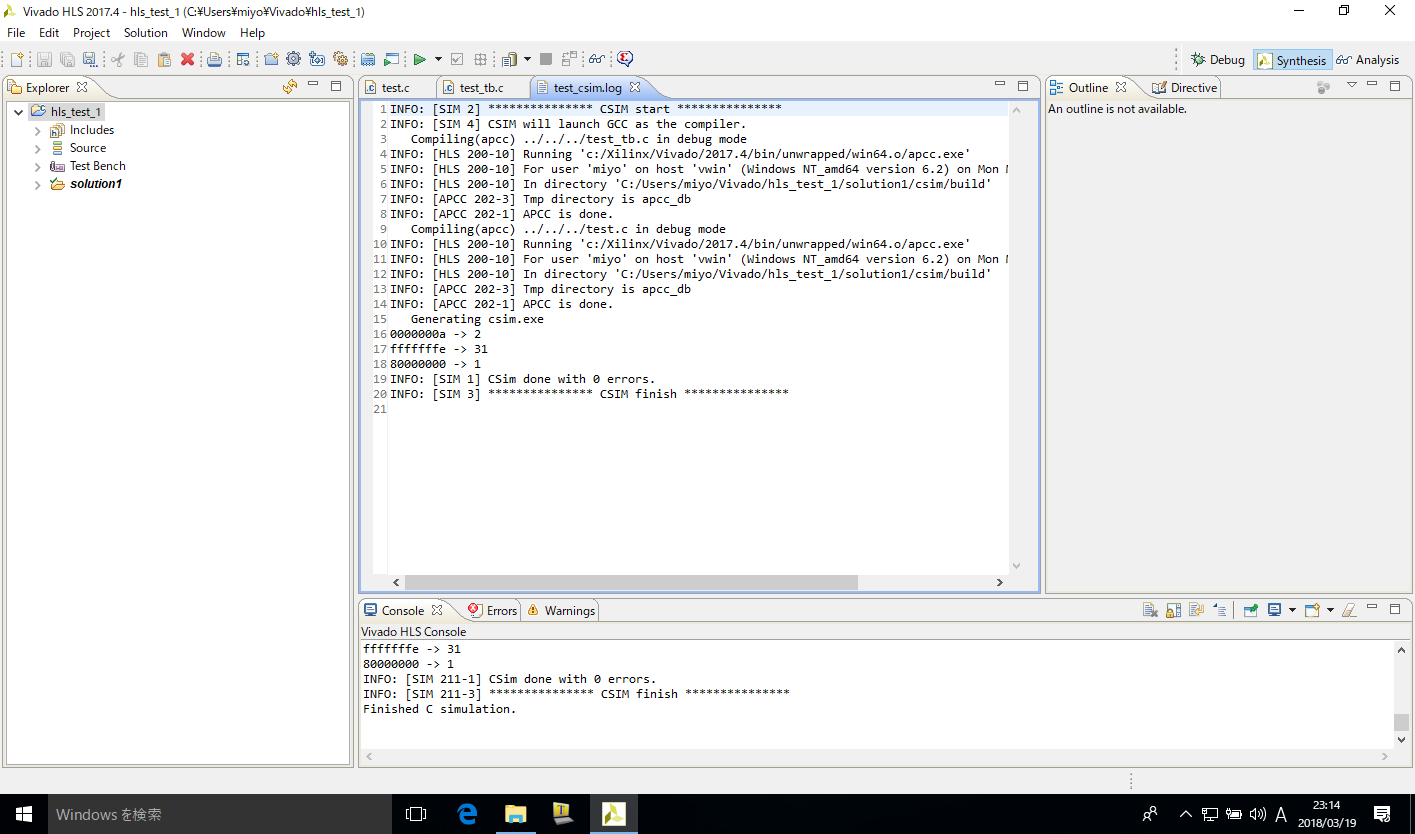
\includegraphics[width=.8\textwidth]{chapter08_figures/VirtualBox_Windows10_19_03_2018_23_17_17.png}
  \end{center}
  \caption{しばらくすると結果が表示される.たとえば0xaの立っているビットは2個で答えが正しいことが確認できた}
 \end{figure}

 \begin{figure}[H]
  \begin{center}
   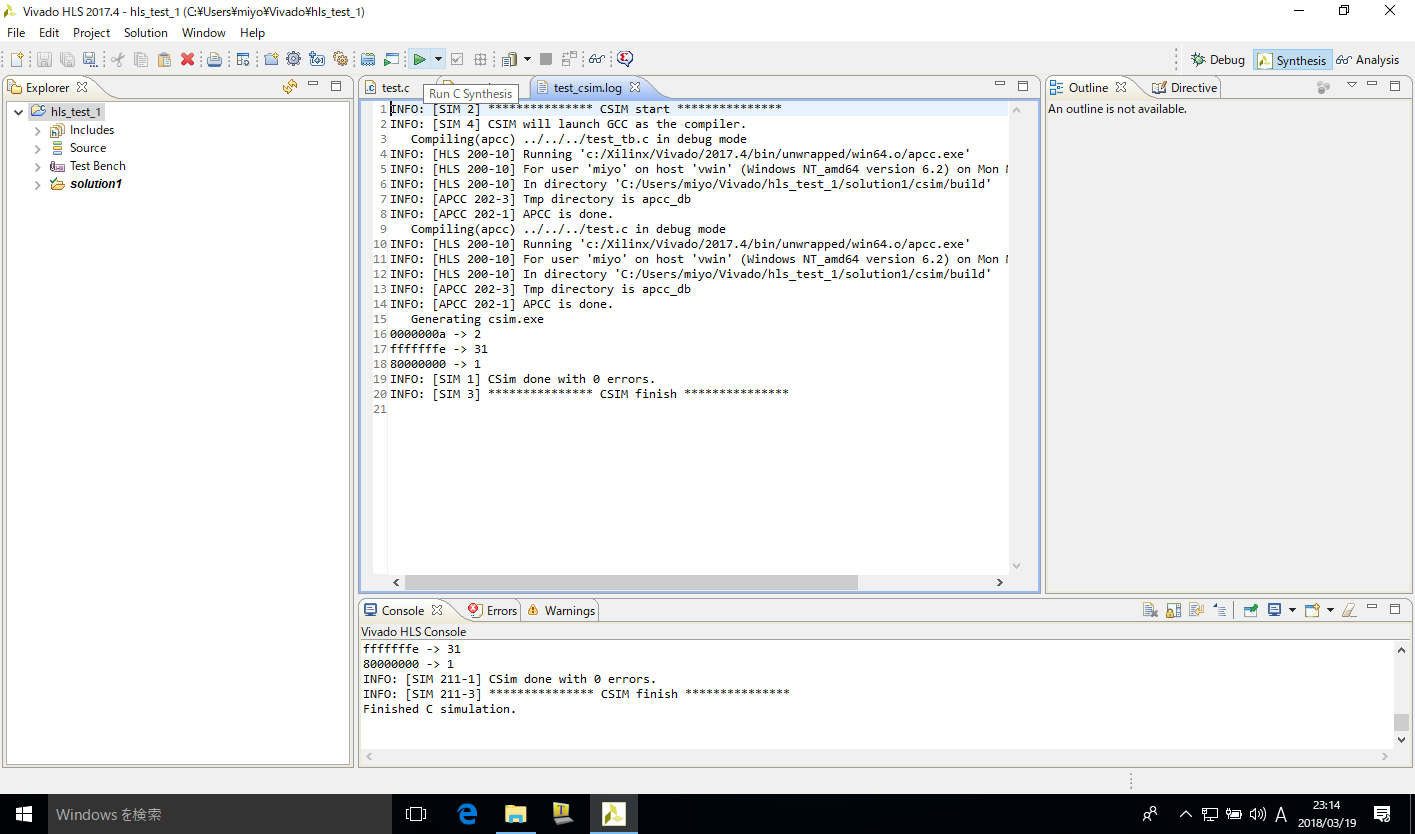
\includegraphics[width=.8\textwidth]{chapter08_figures/VirtualBox_Windows10_19_03_2018_23_17_41.png}
  \end{center}
  \caption{ツールバーの再生ボタンアイコンをクリックしてCからHDLの合成を開始する}
 \end{figure}

 \begin{figure}[H]
  \begin{center}
   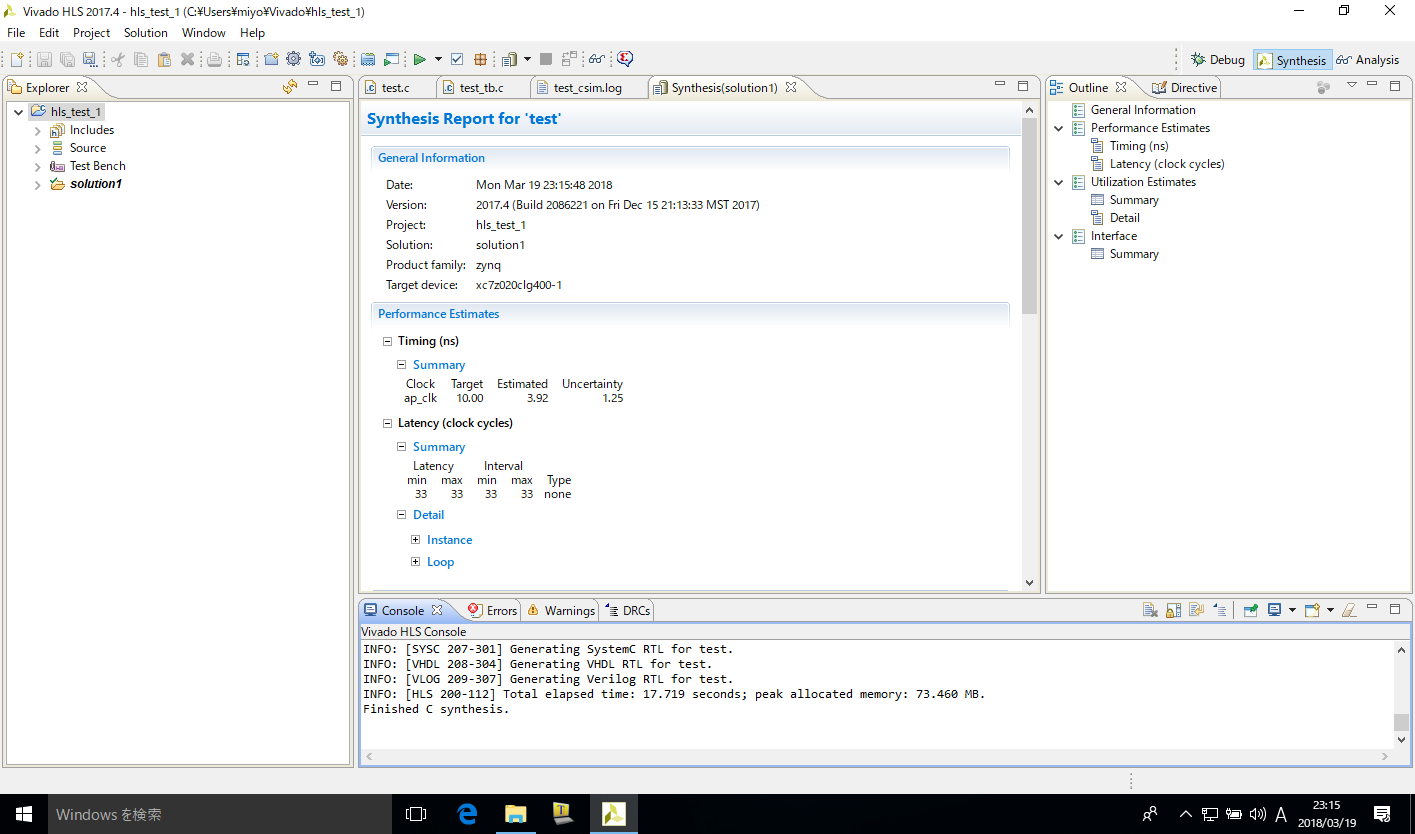
\includegraphics[width=.8\textwidth]{chapter08_figures/VirtualBox_Windows10_19_03_2018_23_18_16.png}
  \end{center}
  \caption{しばらく待つと合成が完了する.ここでは生成された回路のクリティカルパス遅延が3.92nsであると表示されている.また,ひとつの答えを得るために33サイクル必要であることも確認できる.}
 \end{figure}

 \begin{figure}[H]
  \begin{center}
   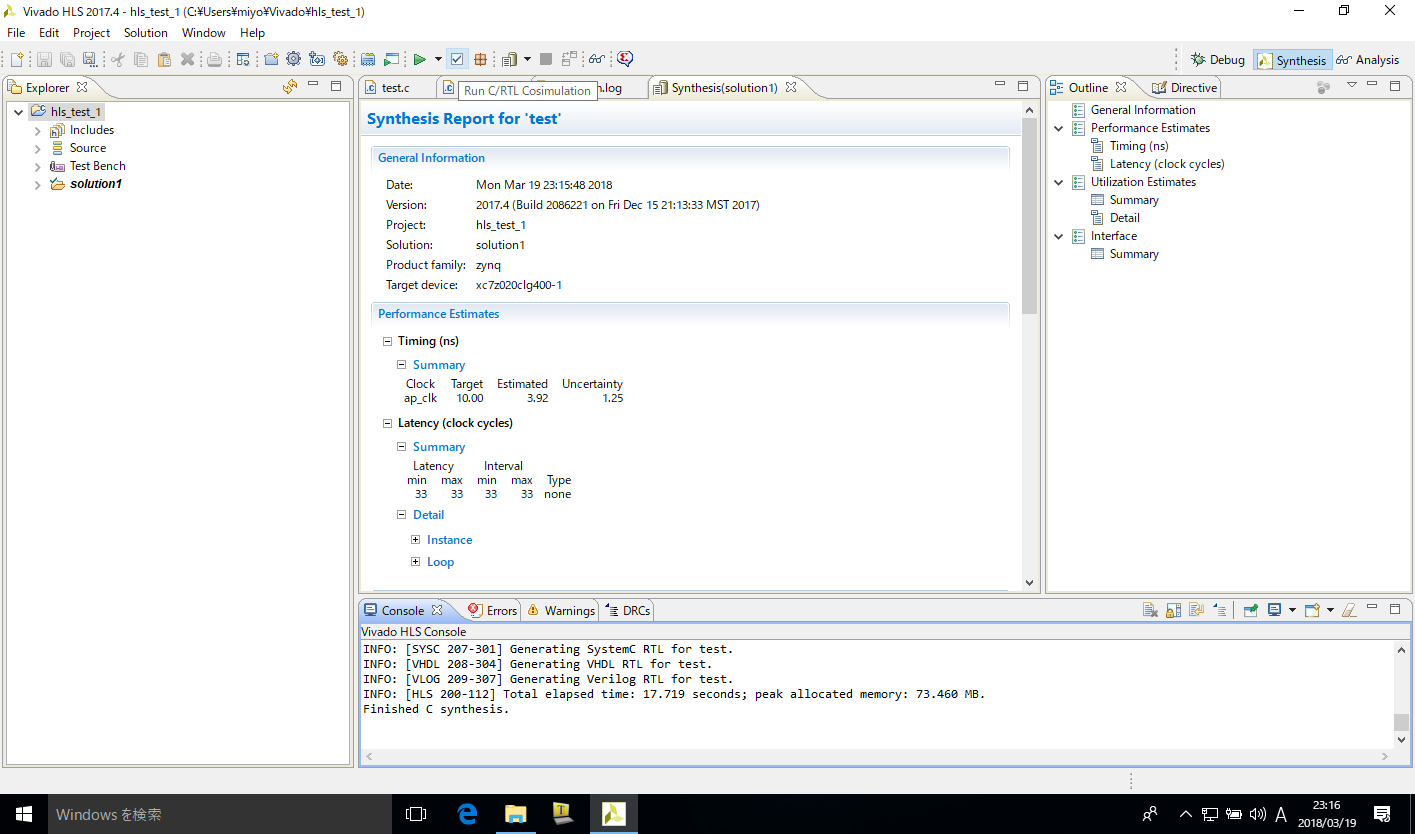
\includegraphics[width=.8\textwidth]{chapter08_figures/VirtualBox_Windows10_19_03_2018_23_18_47.png}
  \end{center}
  \caption{合成したHDLの動作検証を行う.テストベンチはCシミュレーションのときと同じ}
 \end{figure}

 \begin{figure}[H]
  \begin{center}
   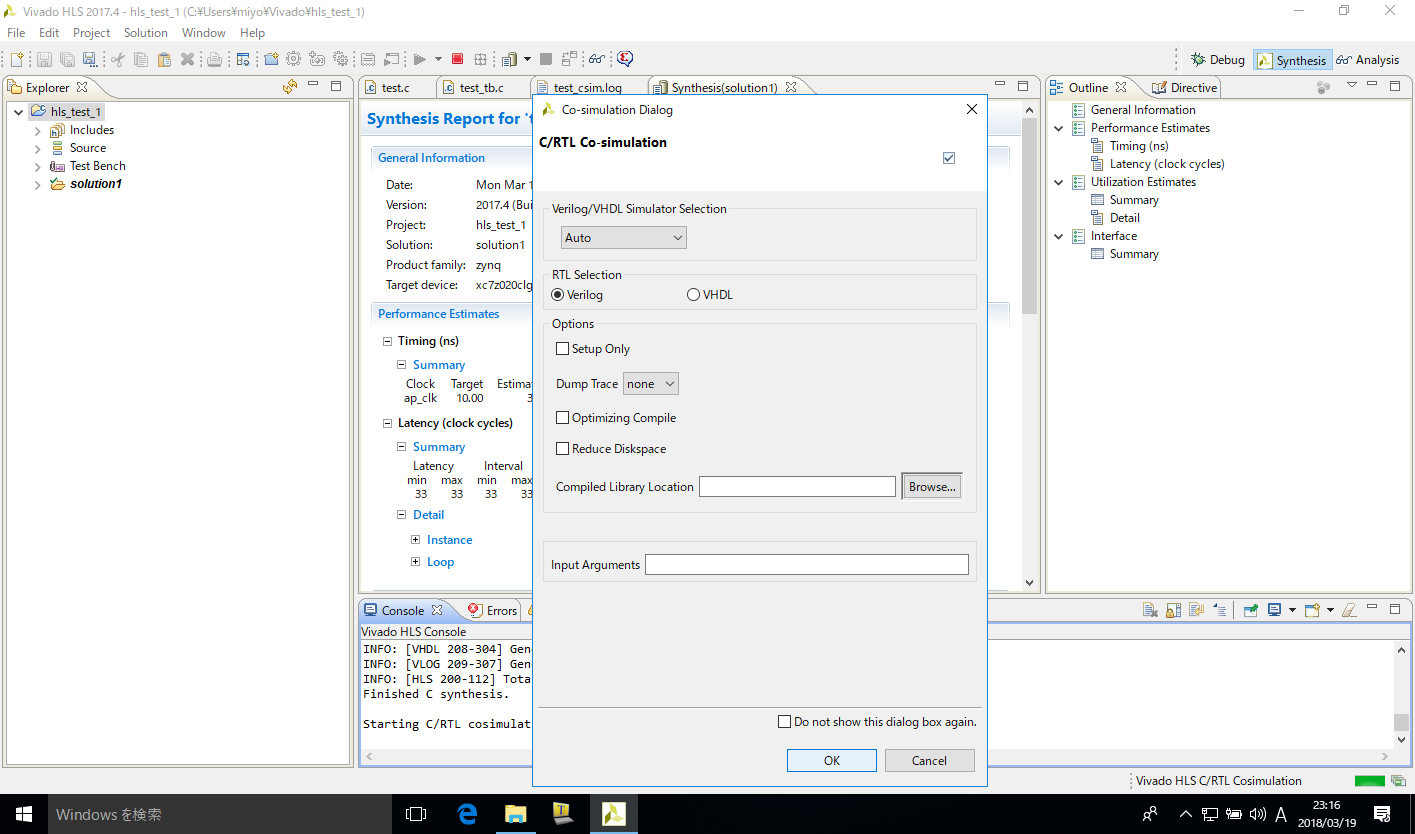
\includegraphics[width=.8\textwidth]{chapter08_figures/VirtualBox_Windows10_19_03_2018_23_18_57.png}
  \end{center}
  \caption{特にオプションは指定せずにOKをクリック}
 \end{figure}

 \begin{figure}[H]
  \begin{center}
   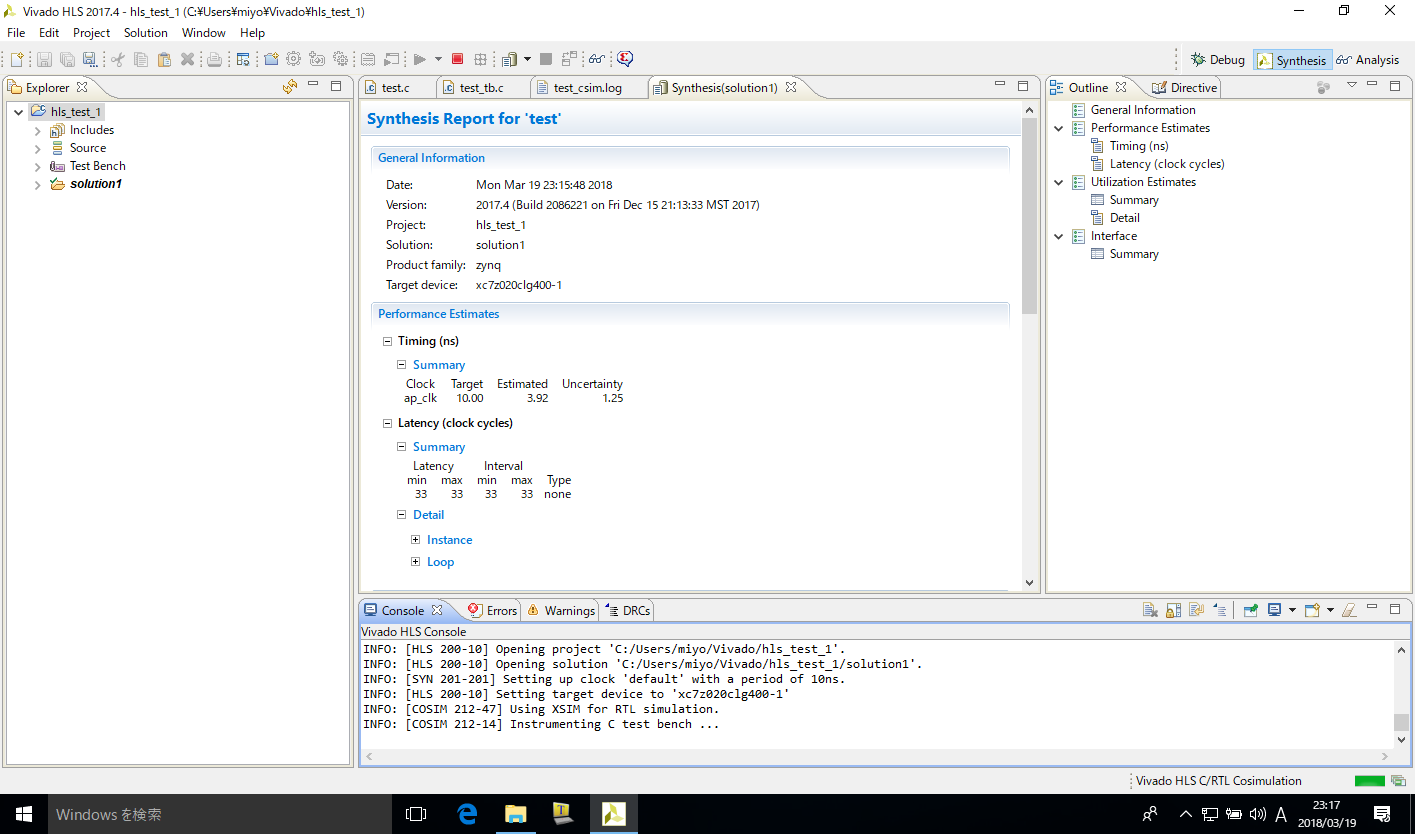
\includegraphics[width=.8\textwidth]{chapter08_figures/VirtualBox_Windows10_19_03_2018_23_19_18.png}
  \end{center}
  \caption{シミュレーションにXSIM(RTLシミュレータ)が使用されていることがわかる}
 \end{figure}

 \begin{figure}[H]
  \begin{center}
   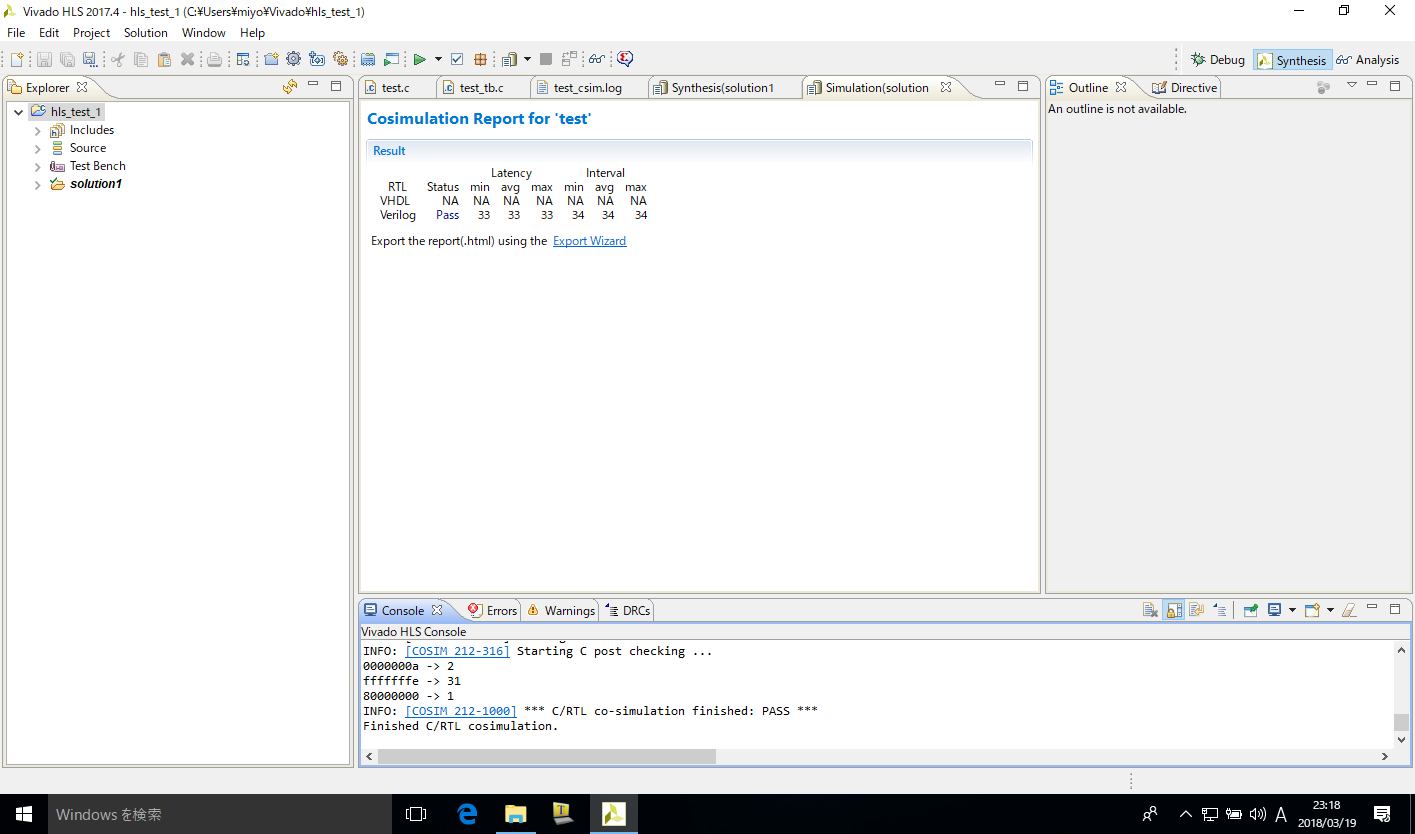
\includegraphics[width=.8\textwidth]{chapter08_figures/VirtualBox_Windows10_19_03_2018_23_20_14.png}
  \end{center}
  \caption{RTLシミュレーションでも望み通りの答えがえられることが確認できた}
 \end{figure}

  \subsection{IPコアの生成}

 \begin{figure}[H]
  \begin{center}
   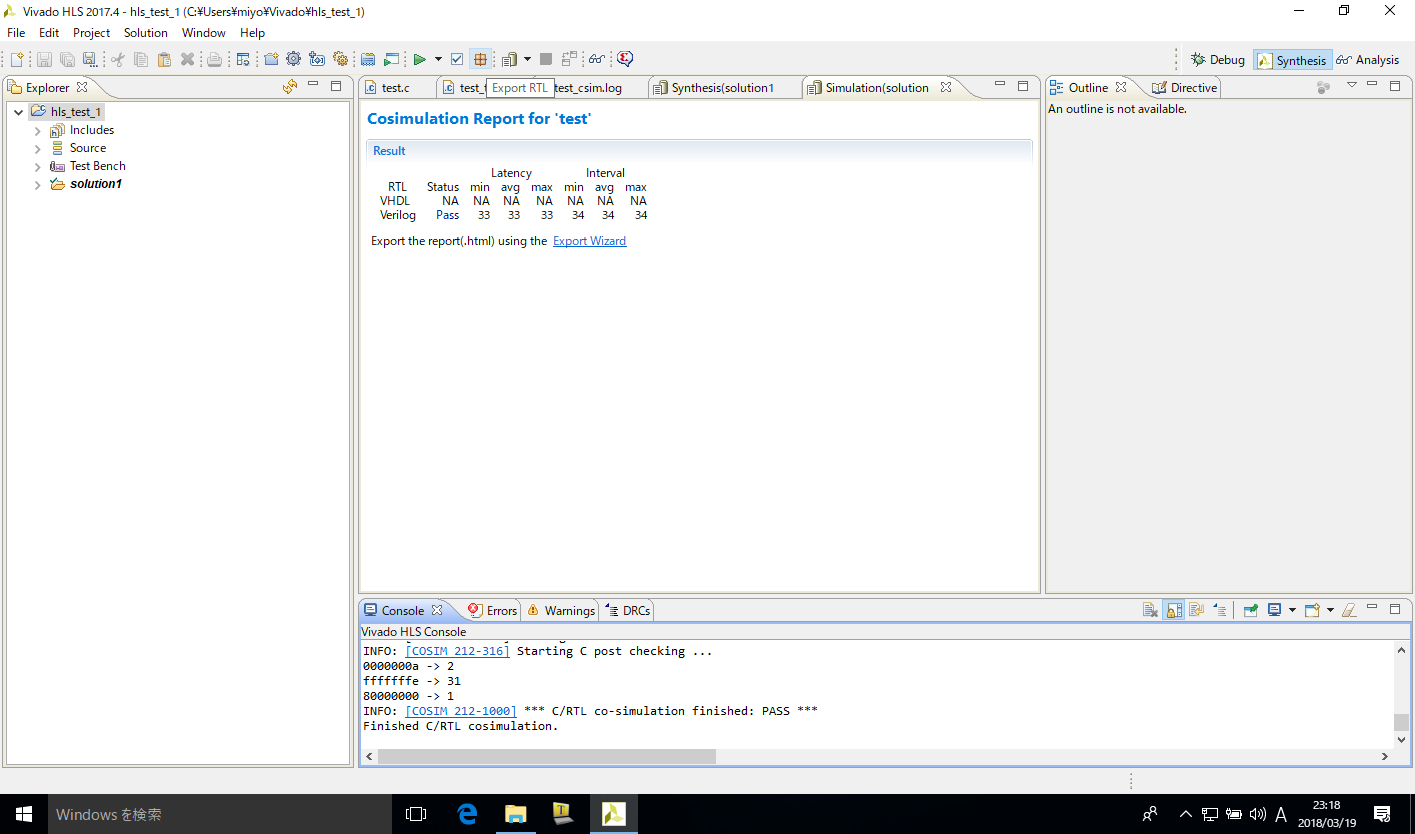
\includegraphics[width=.8\textwidth]{chapter08_figures/VirtualBox_Windows10_19_03_2018_23_20_28.png}
  \end{center}
  \caption{ツールバーの荷物のようなアイコンをクリックしてIPコアを生成する}
 \end{figure}

 \begin{figure}[H]
  \begin{center}
   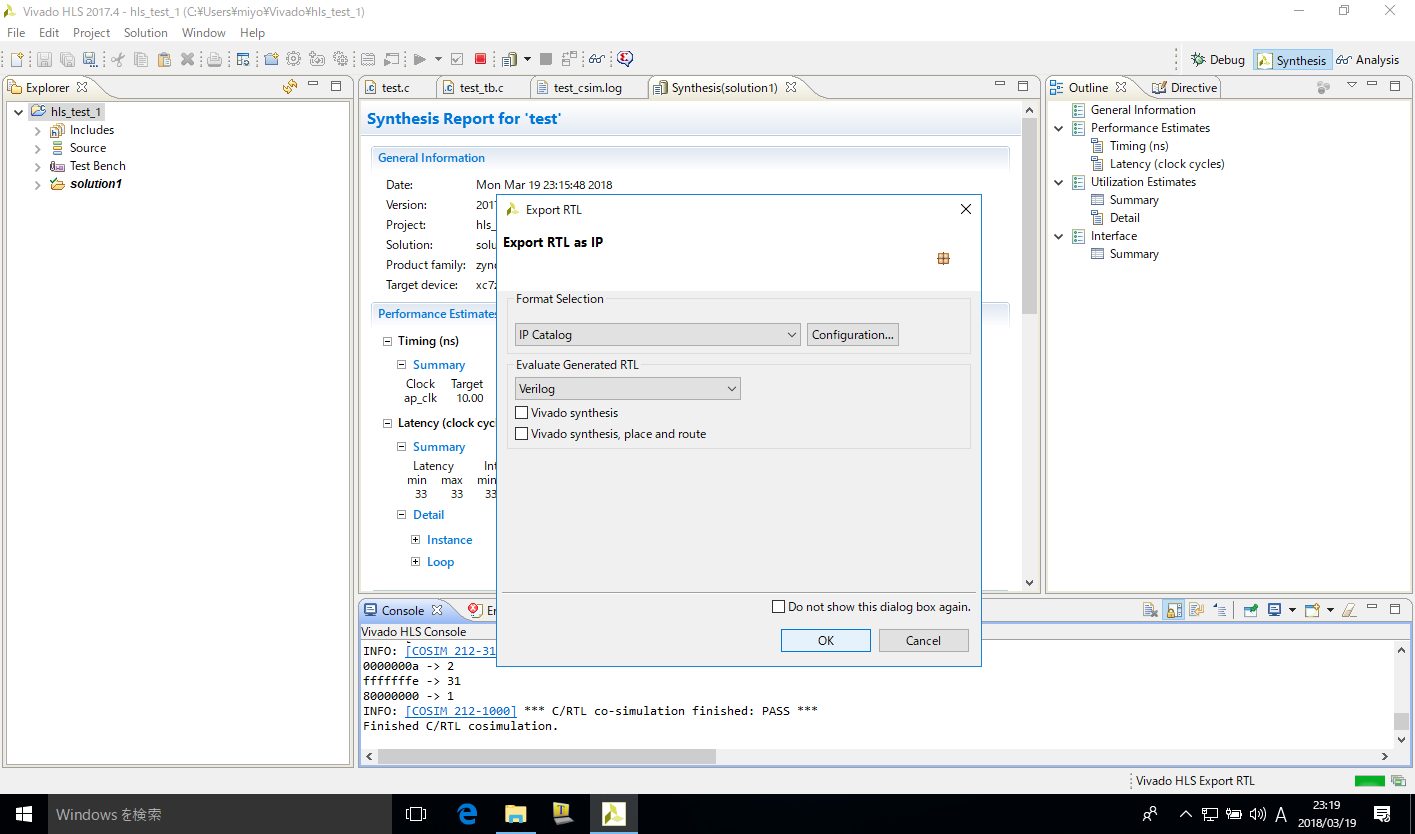
\includegraphics[width=.8\textwidth]{chapter08_figures/VirtualBox_Windows10_19_03_2018_23_21_04.png}
  \end{center}
  \caption{IPコア生成に関する設定ダイアログが開いたところ.特に変更の必要はないのでOKをクリック}
 \end{figure}

 %%
 \begin{figure}[H]
  \begin{center}
   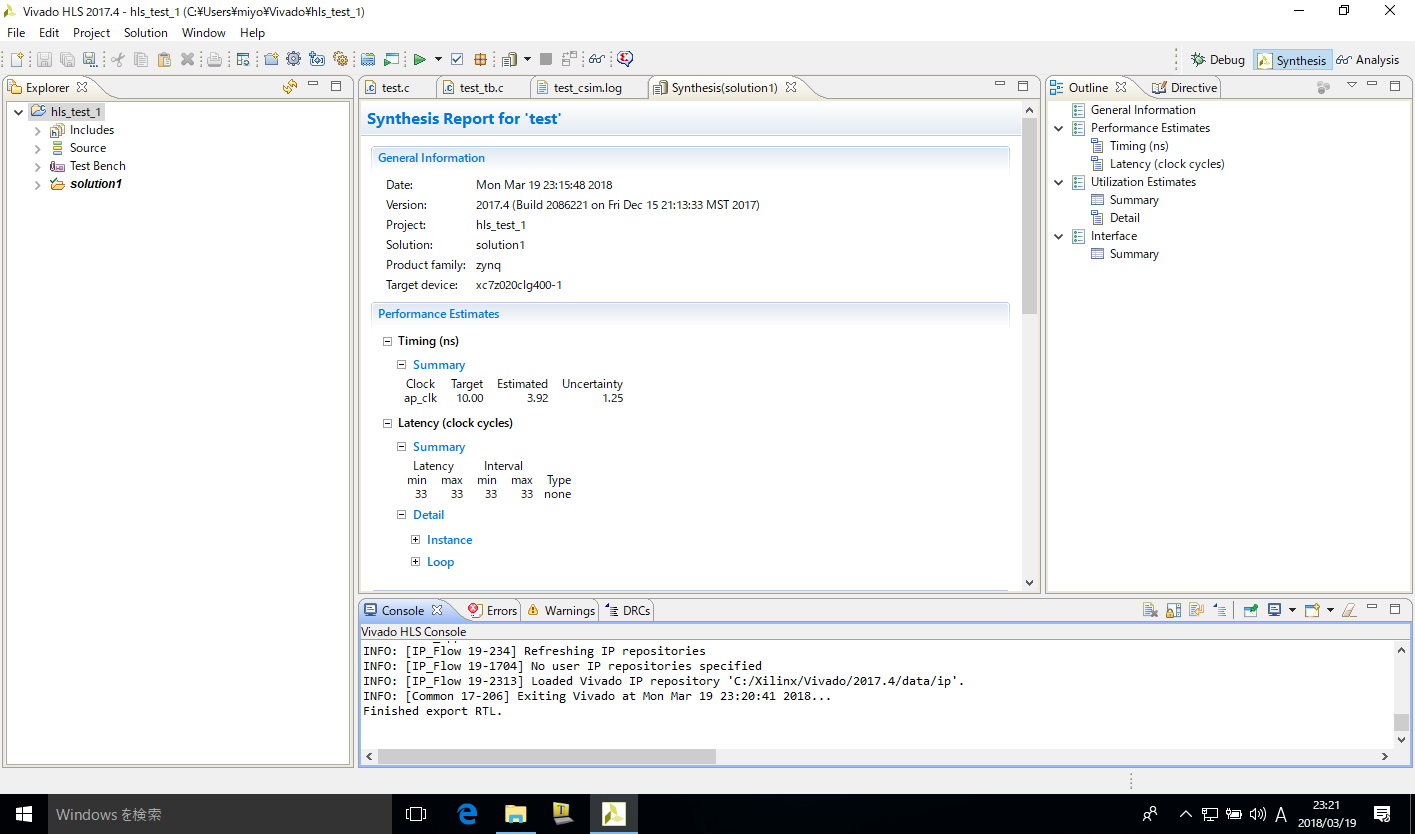
\includegraphics[width=.8\textwidth]{chapter08_figures/VirtualBox_Windows10_19_03_2018_23_21_59.png}
  \end{center}
  \caption{しばらく待つと,Vivadoで利用可能なIPコアが生成される.}
 \end{figure}

 \begin{figure}[H]
  \begin{center}
   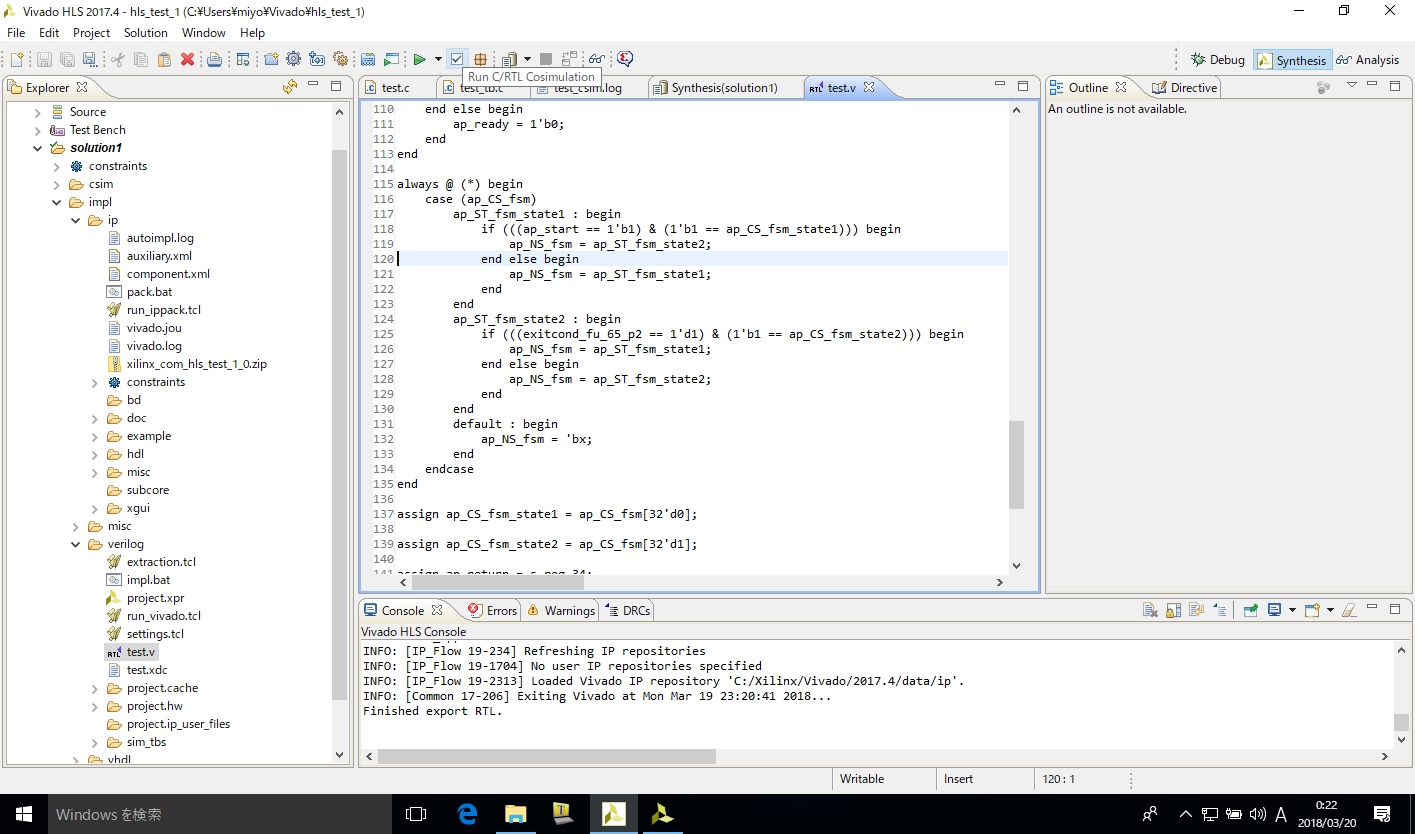
\includegraphics[width=.8\textwidth]{chapter08_figures/VirtualBox_Windows10_20_03_2018_00_22_51.png}
  \end{center}
  \caption{生成されたリソースやファイルはsolution1の下のimplの下に格納されていて自由に確認することができる}
 \end{figure}

 \subsection{生成したモジュールをFPGAプロジェクトで利用する}

 \begin{figure}[H]
  \begin{center}
   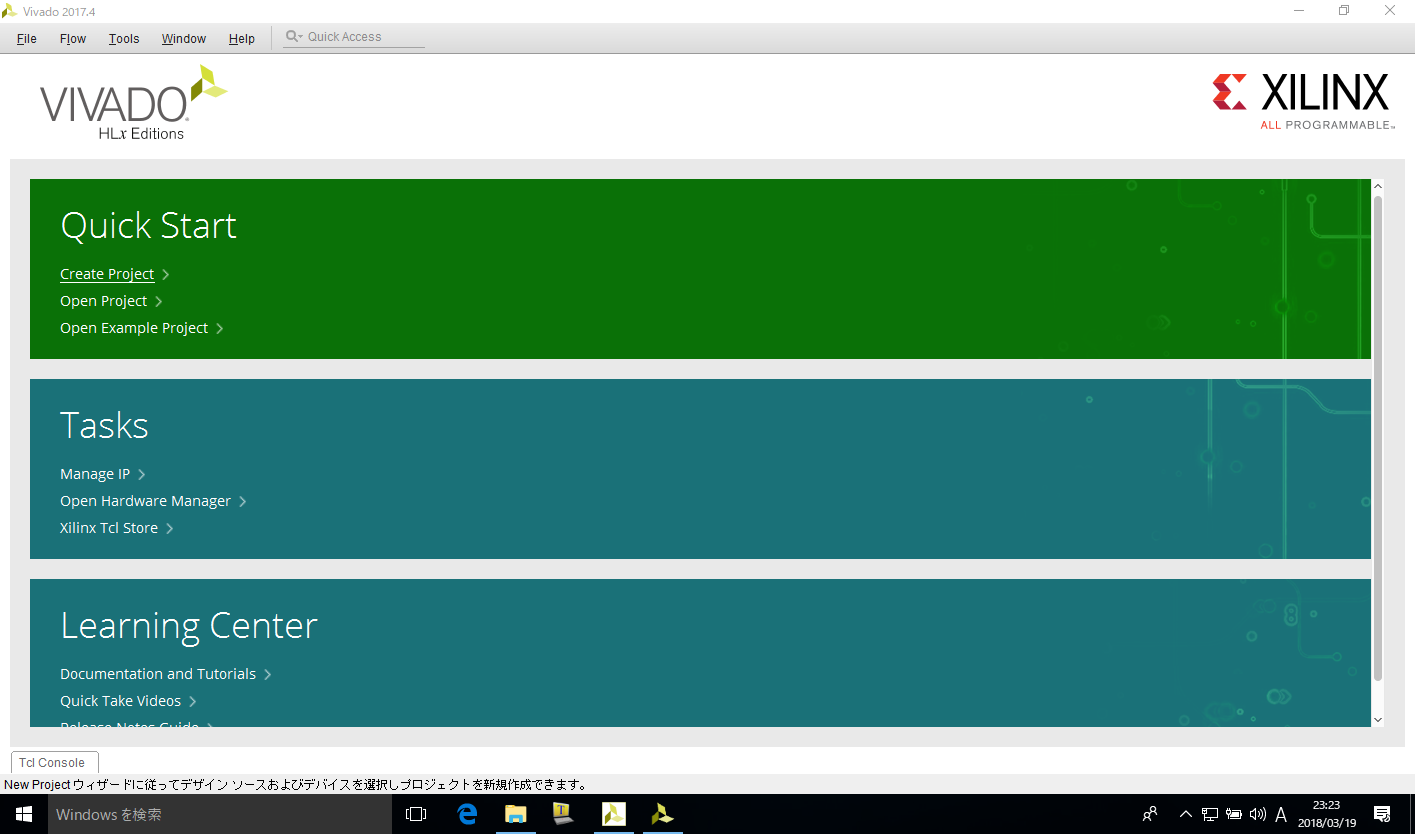
\includegraphics[width=.8\textwidth]{chapter08_figures/VirtualBox_Windows10_19_03_2018_23_23_11.png}
  \end{center}
  \caption{まずはVivadoプロジェクトを作成する}
 \end{figure}

 \begin{figure}[H]
  \begin{center}
   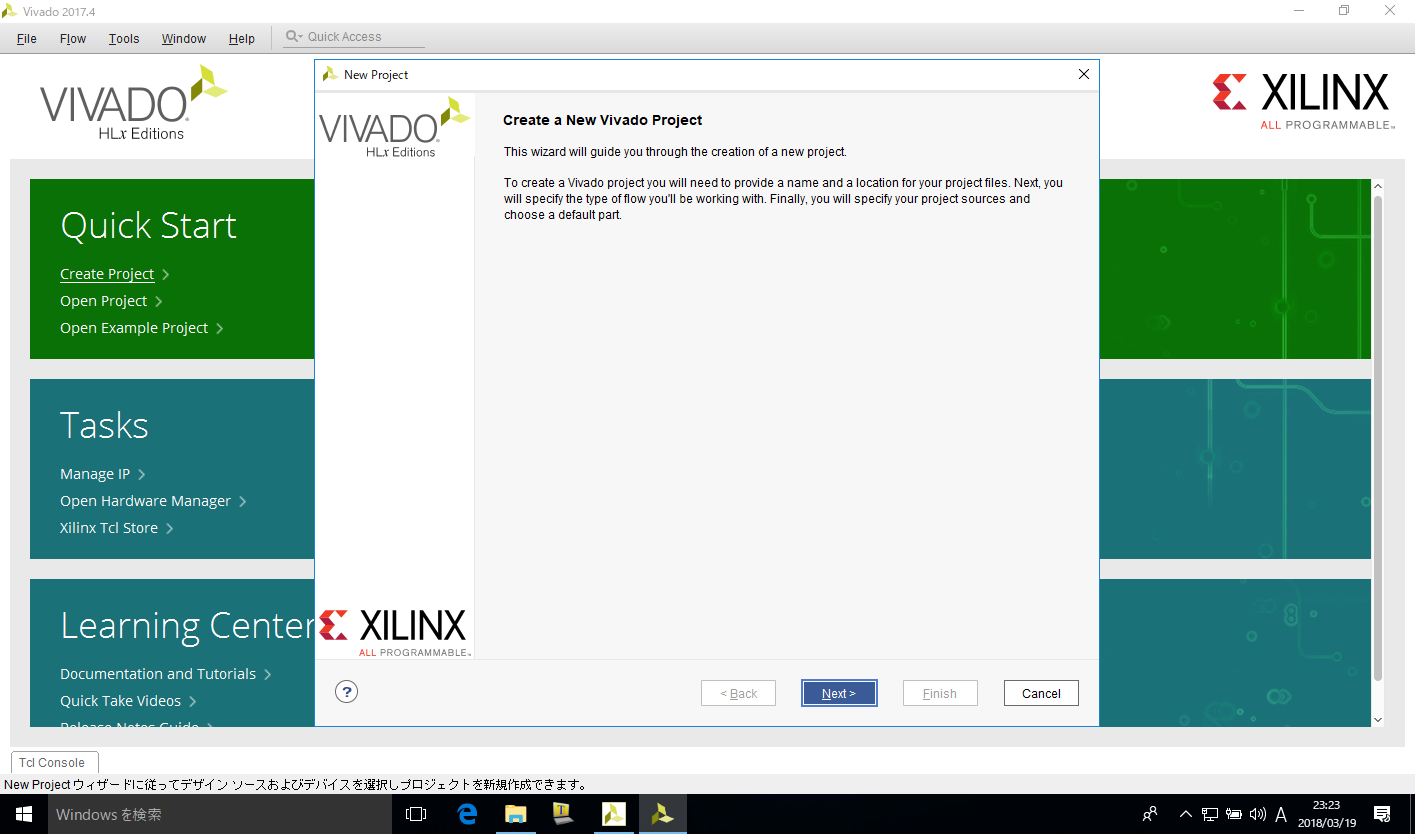
\includegraphics[width=.8\textwidth]{chapter08_figures/VirtualBox_Windows10_19_03_2018_23_23_20.png}
  \end{center}
  \caption{プロジェクト作成ダイアログ.Nextで次へ}
 \end{figure}

 \begin{figure}[H]
  \begin{center}
   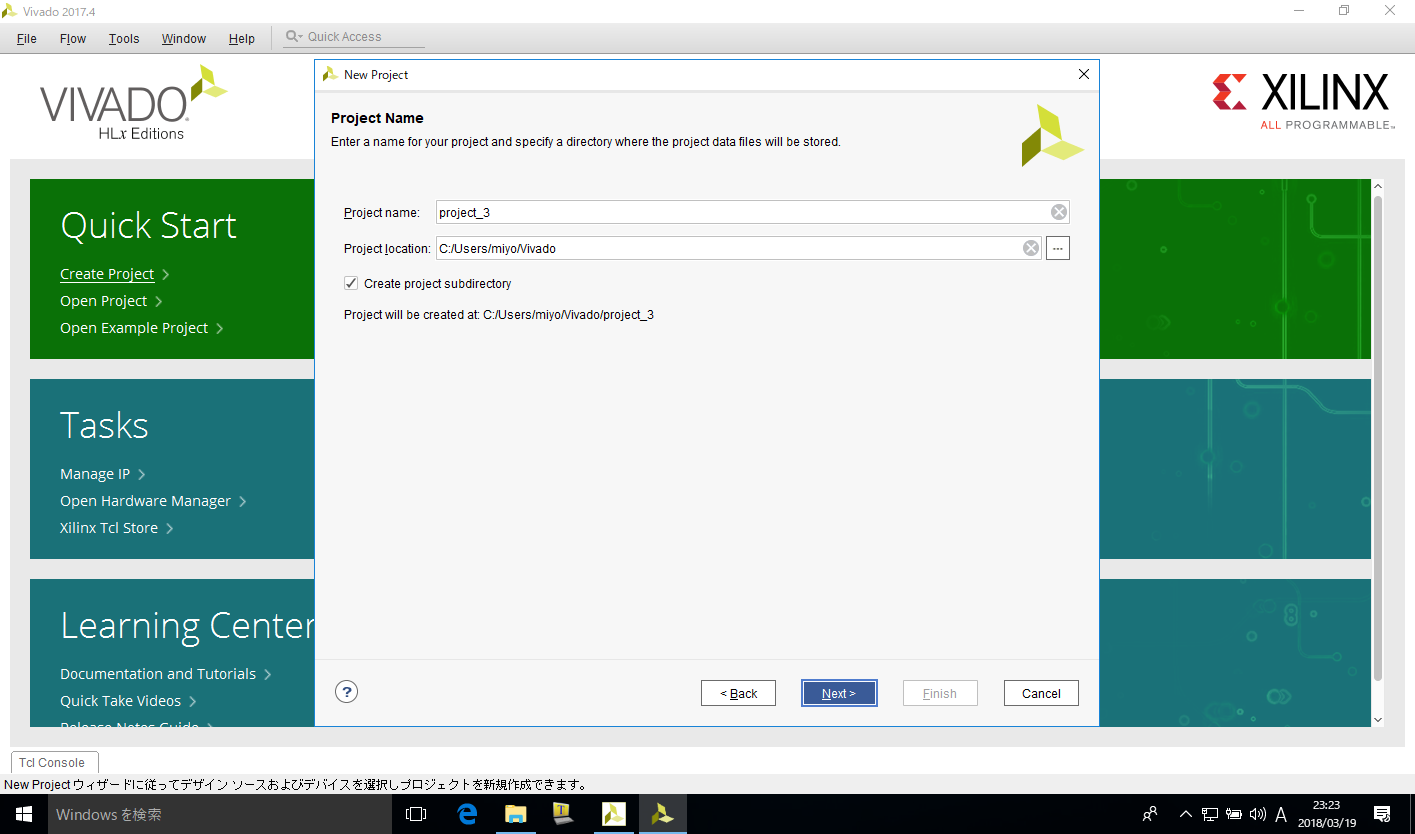
\includegraphics[width=.8\textwidth]{chapter08_figures/VirtualBox_Windows10_19_03_2018_23_23_26.png}
  \end{center}
  \caption{プロジェクト名をproject\_3として,ホーム下のVivadoフォルダの下に保存することにする}
 \end{figure}

 \begin{figure}[H]
  \begin{center}
   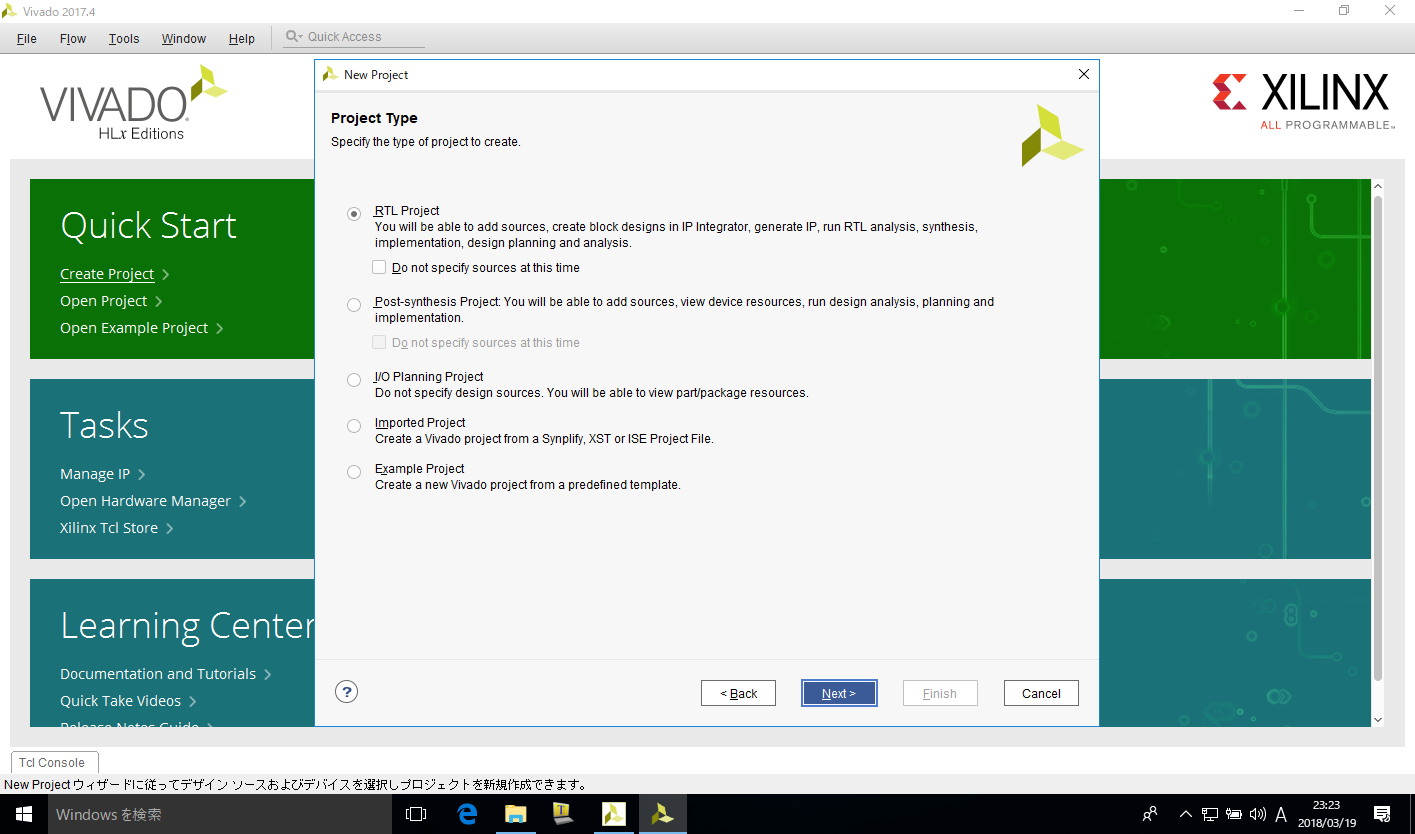
\includegraphics[width=.8\textwidth]{chapter08_figures/VirtualBox_Windows10_19_03_2018_23_23_30.png}
  \end{center}
  \caption{作成するプロジェクトはRTLプロジェクトを選択.}
 \end{figure}

 \begin{figure}[H]
  \begin{center}
   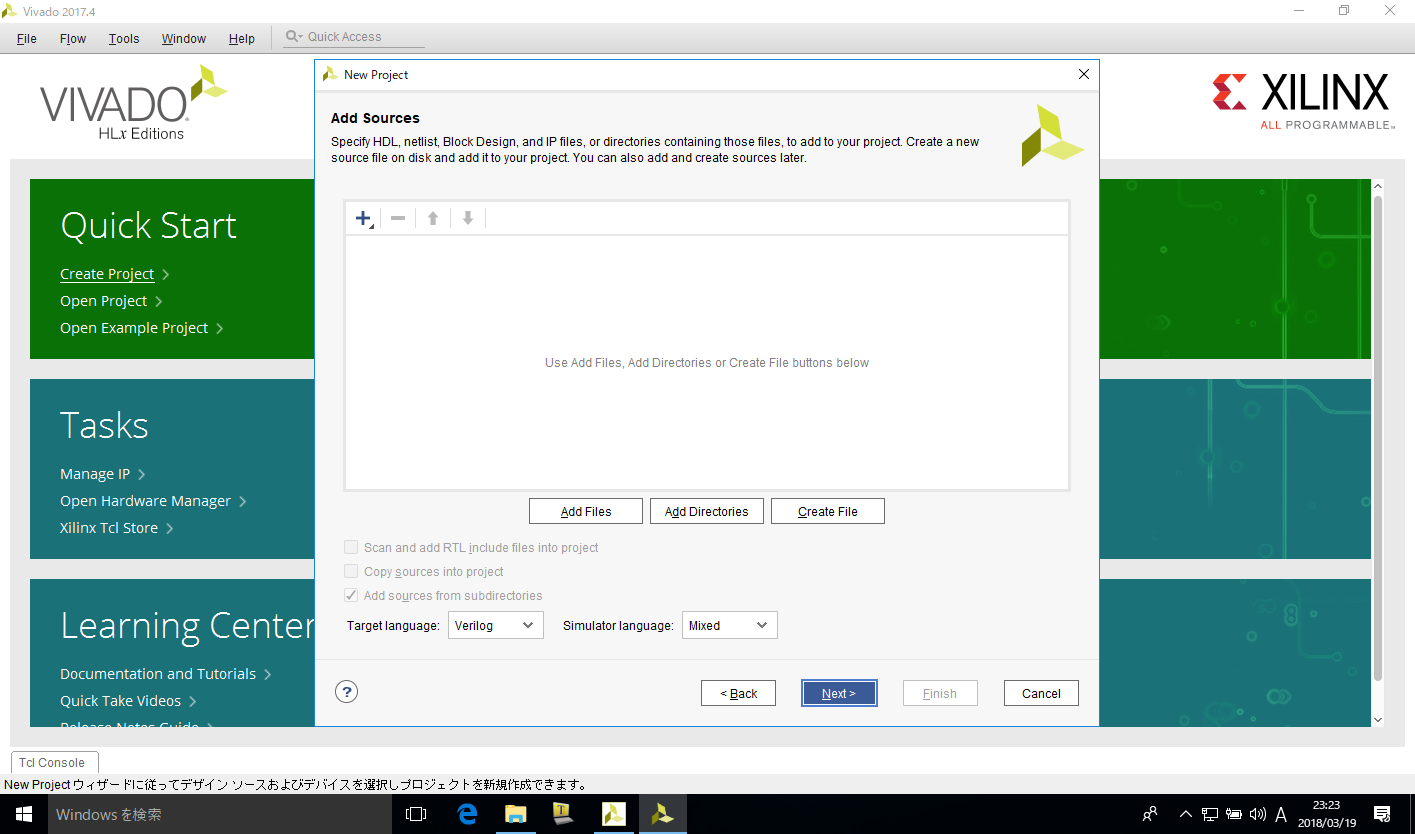
\includegraphics[width=.8\textwidth]{chapter08_figures/VirtualBox_Windows10_19_03_2018_23_23_35.png}
  \end{center}
  \caption{特にここで追加するファイルはないのでNextで次へ}
 \end{figure}

 \begin{figure}[H]
  \begin{center}
   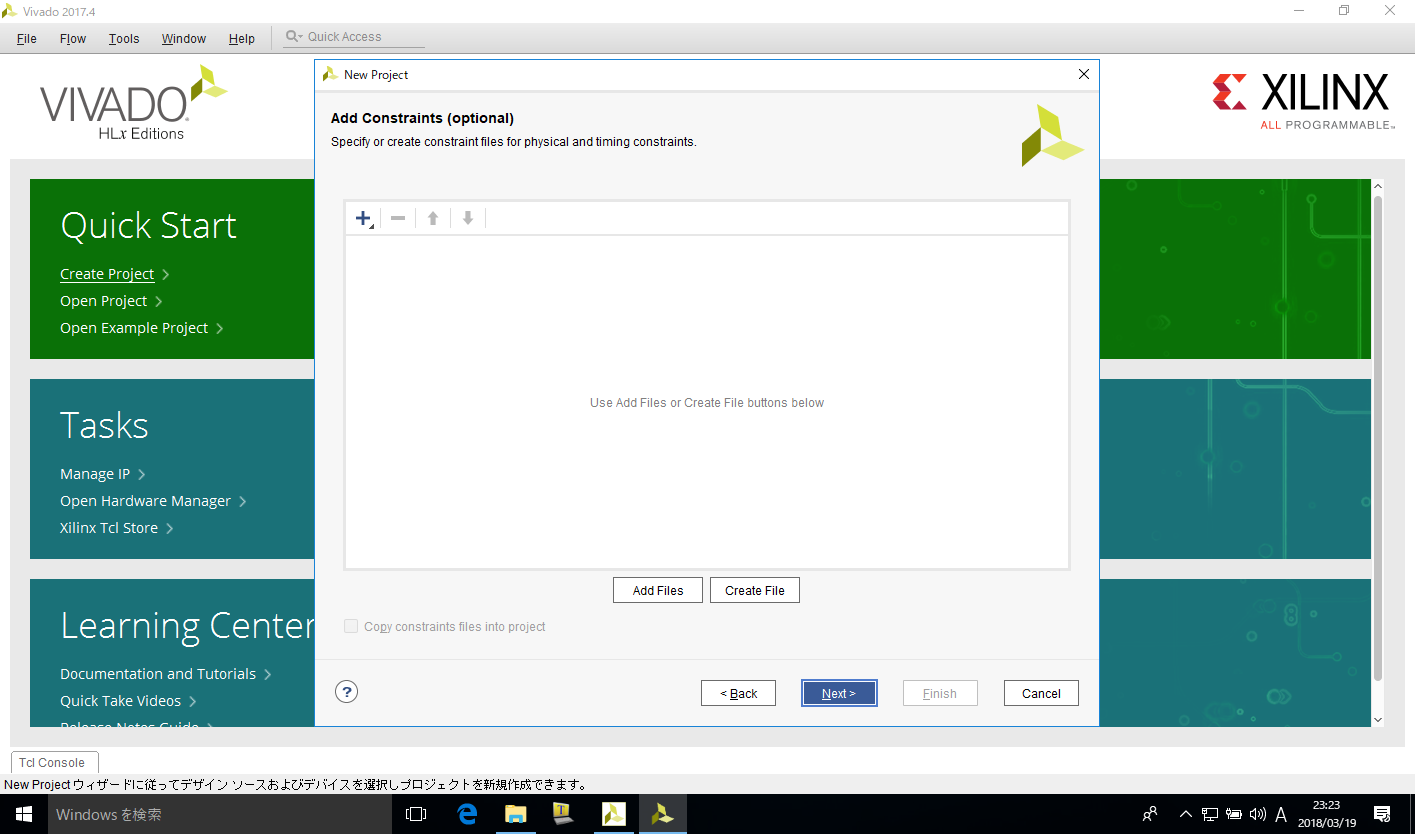
\includegraphics[width=.8\textwidth]{chapter08_figures/VirtualBox_Windows10_19_03_2018_23_23_39.png}
  \end{center}
  \caption{特にここで追加するファイルはないのでNextで次へ}
 \end{figure}

 \begin{figure}[H]
  \begin{center}
   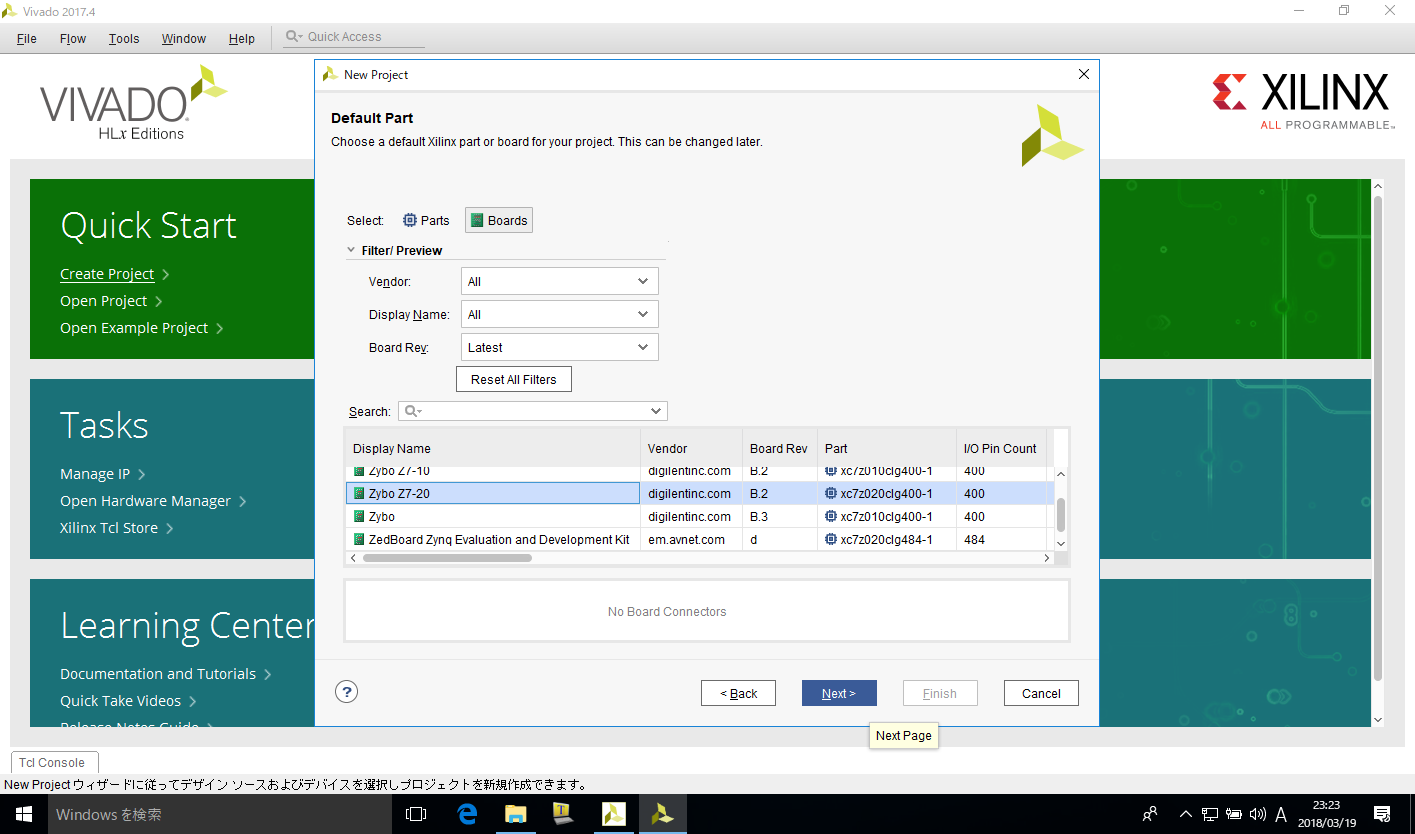
\includegraphics[width=.8\textwidth]{chapter08_figures/VirtualBox_Windows10_19_03_2018_23_23_52.png}
  \end{center}
  \caption{プロジェクトの開発ターゲットはボードリストからZybo Z7-20を選択}
 \end{figure}

 %%
 \begin{figure}[H]
  \begin{center}
   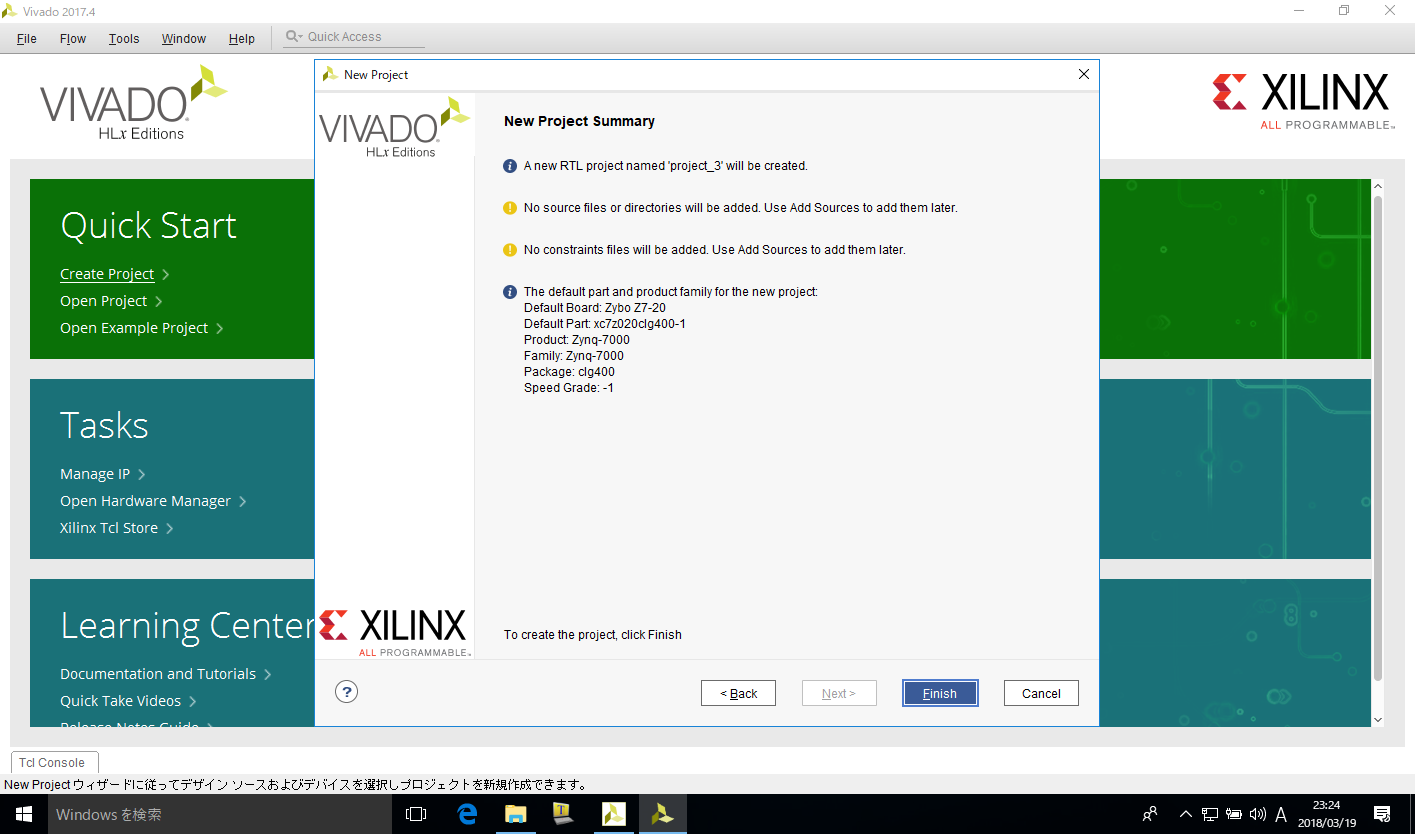
\includegraphics[width=.8\textwidth]{chapter08_figures/VirtualBox_Windows10_19_03_2018_23_23_58.png}
  \end{center}
  \caption{設定内容を確認してFinishをクリック.ウィザードを終了する.}
 \end{figure}

 \begin{figure}[H]
  \begin{center}
   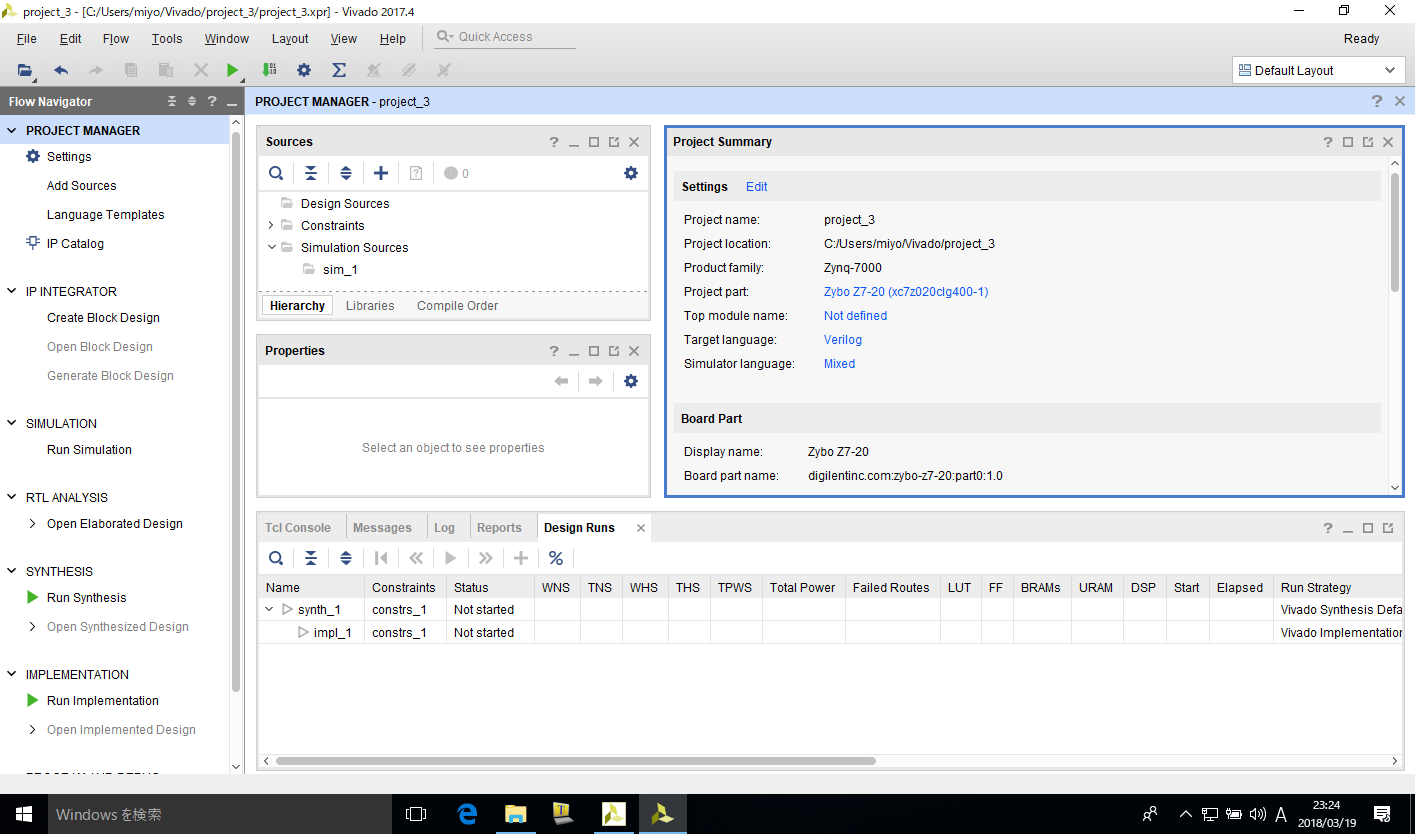
\includegraphics[width=.8\textwidth]{chapter08_figures/VirtualBox_Windows10_19_03_2018_23_24_25.png}
  \end{center}
  \caption{PROJECT NAVIGATORのSettingsをクリックして設定画面を呼び出す}
 \end{figure}

 \begin{figure}[H]
  \begin{center}
   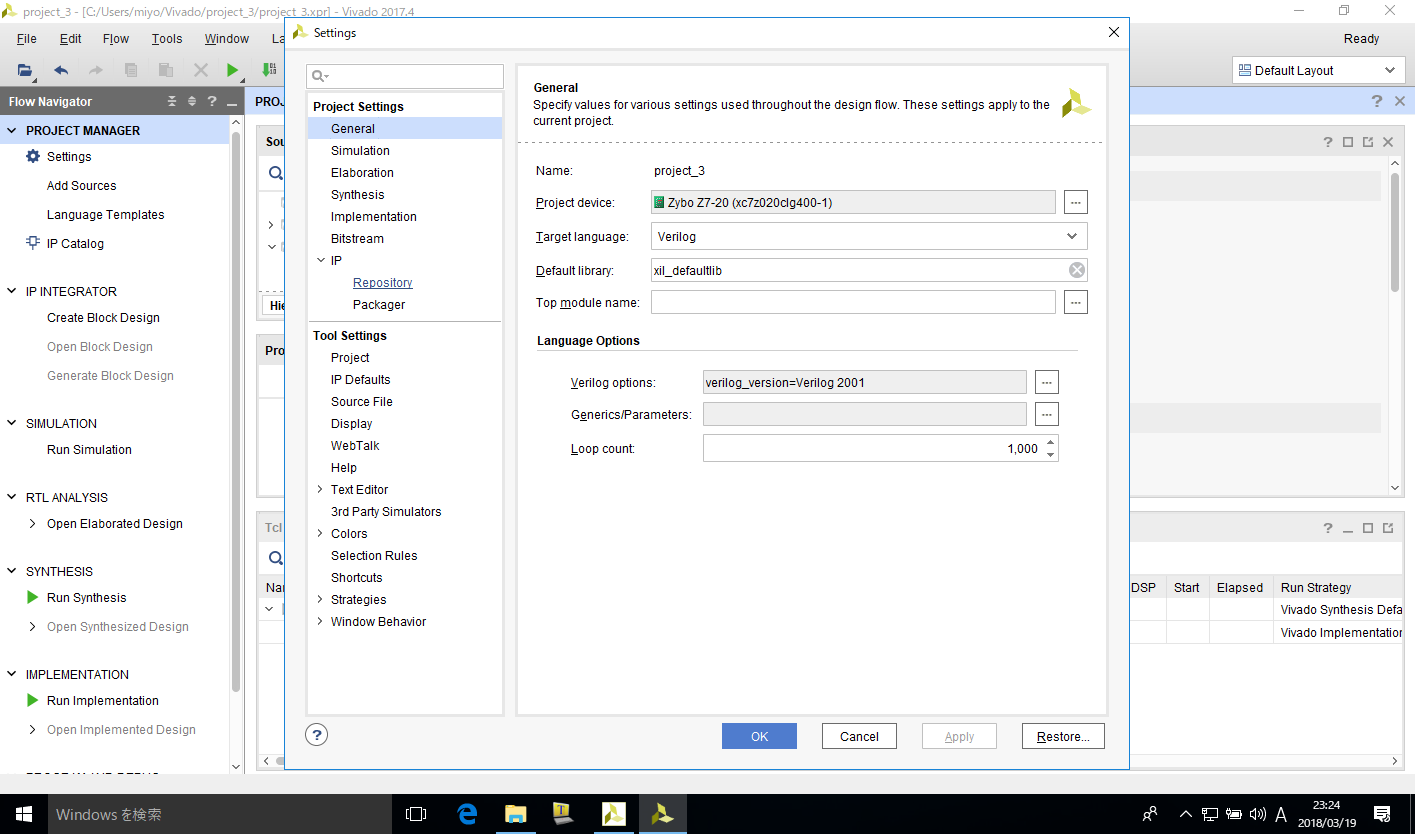
\includegraphics[width=.8\textwidth]{chapter08_figures/VirtualBox_Windows10_19_03_2018_23_24_37.png}
  \end{center}
  \caption{リストのIPを展開し,Repositriesを選択する}
 \end{figure}

 \begin{figure}[H]
  \begin{center}
   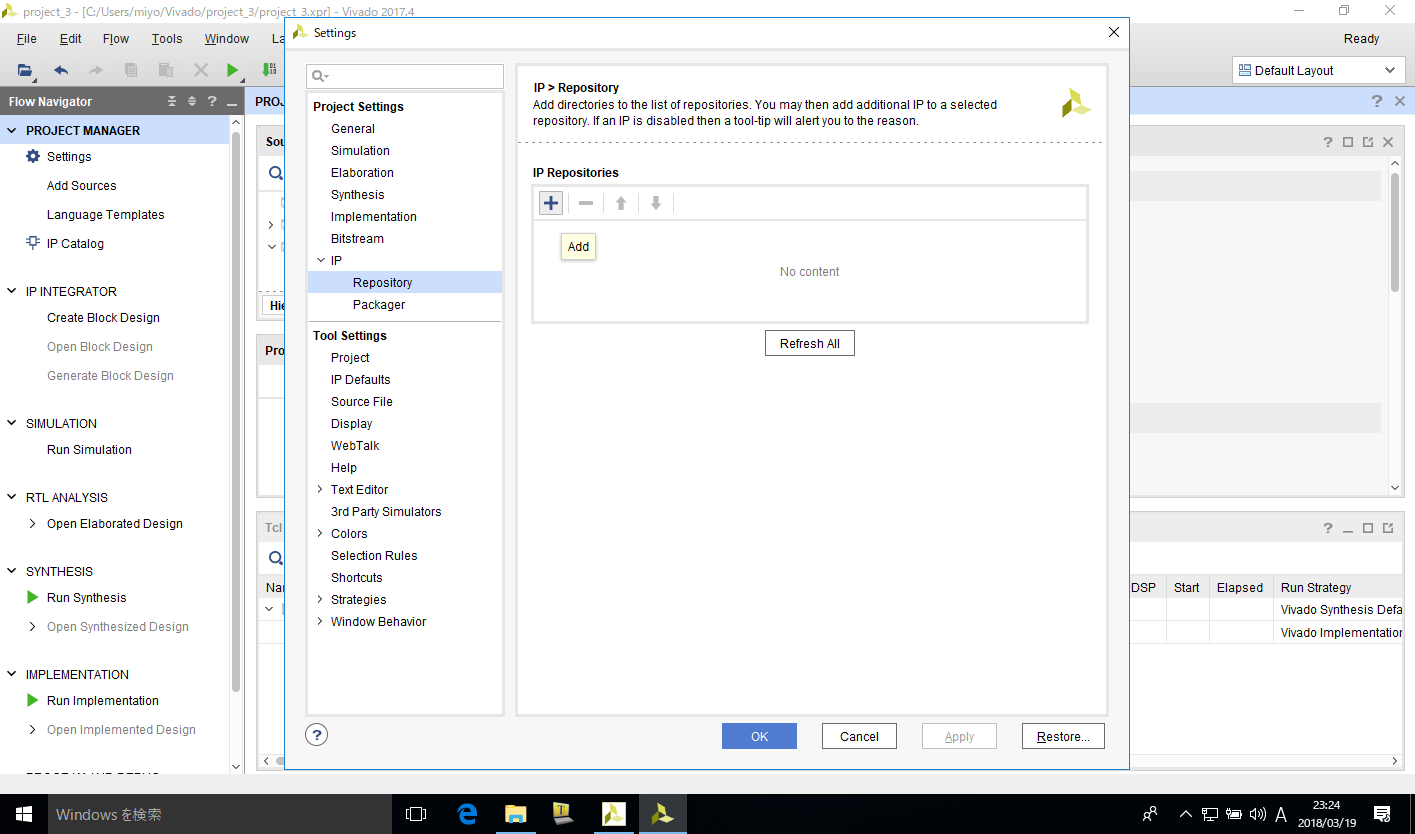
\includegraphics[width=.8\textwidth]{chapter08_figures/VirtualBox_Windows10_19_03_2018_23_24_43.png}
  \end{center}
  \caption{ここにVivado HLSで作成したIPコアのフォルダを指定すれば利用できるようになる.+アイコンをクリック.}
 \end{figure}

 \begin{figure}[H]
  \begin{center}
   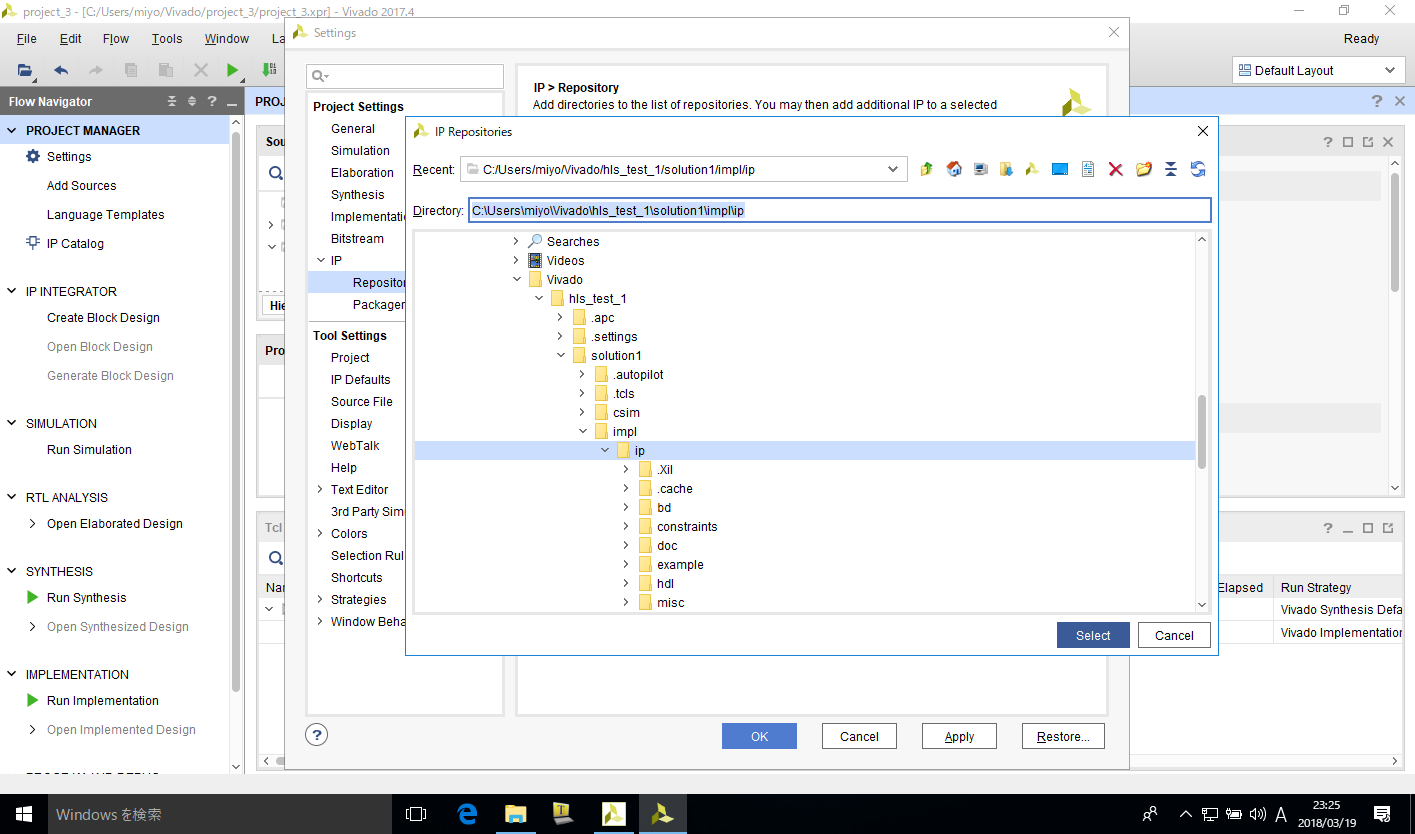
\includegraphics[width=.8\textwidth]{chapter08_figures/VirtualBox_Windows10_19_03_2018_23_25_42.png}
  \end{center}
  \caption{IPコア検索用のフォルダとしてVivado HLSで作成したプロジェクトフォルダ(hls\_test\_1)の下の,solusion1\yen ipを選択して,Selectをクリック}
 \end{figure}

 \begin{figure}[H]
  \begin{center}
   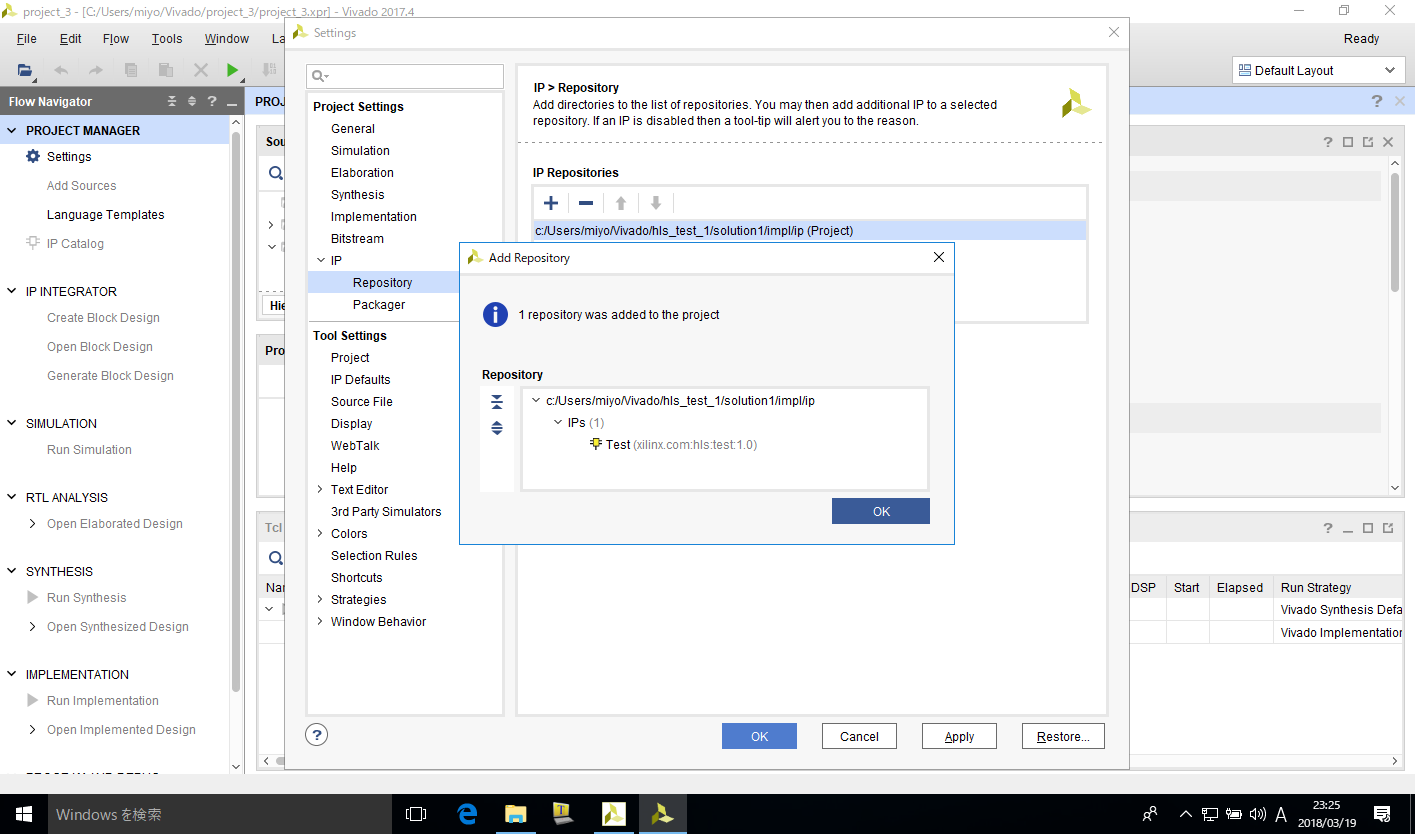
\includegraphics[width=.8\textwidth]{chapter08_figures/VirtualBox_Windows10_19_03_2018_23_25_53.png}
  \end{center}
  \caption{追加したリポジトリ情報が表示される.TestというIPコアが含まれていれば設定は正しい.OKでダイアログを閉じる}
 \end{figure}

 \begin{figure}[H]
  \begin{center}
   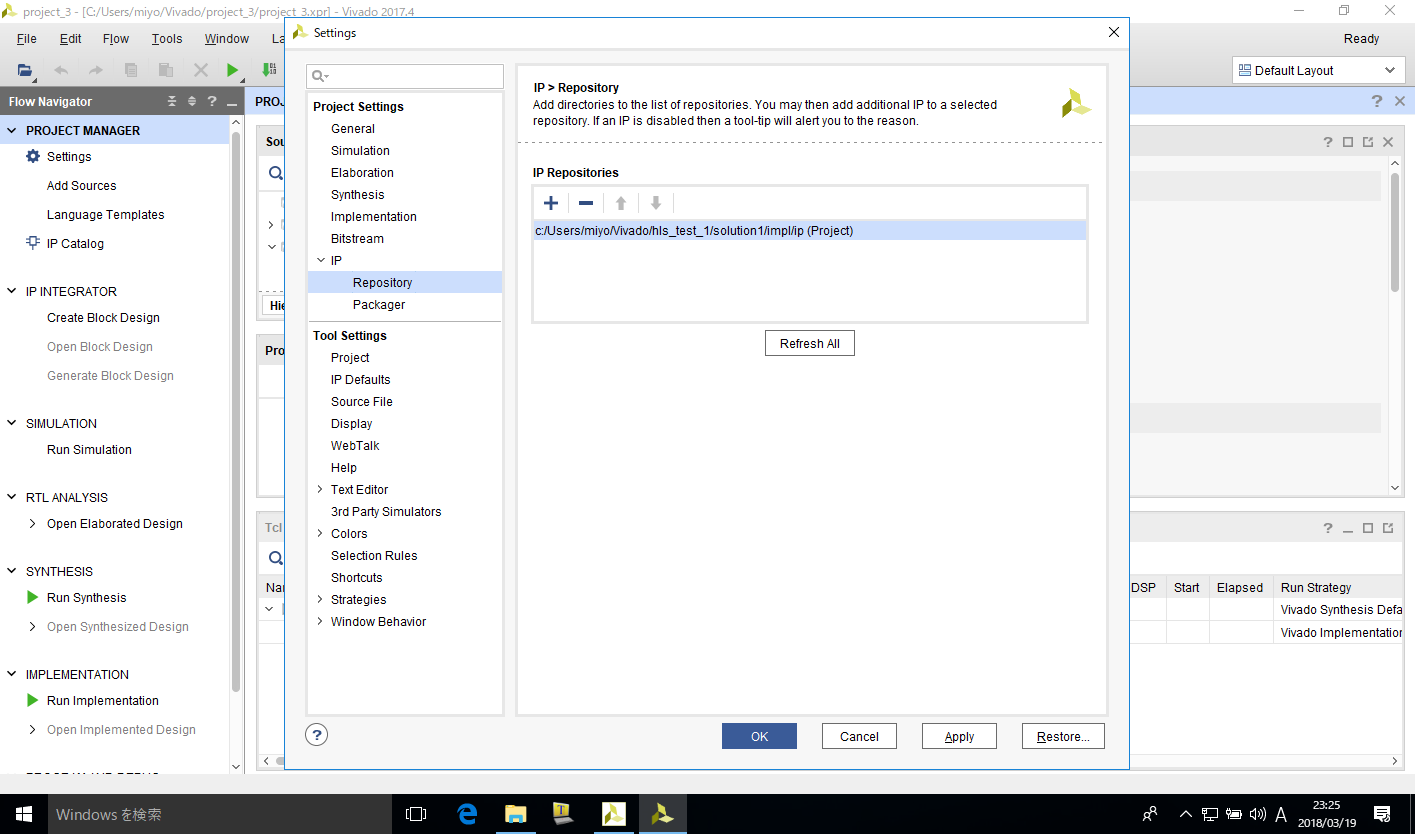
\includegraphics[width=.8\textwidth]{chapter08_figures/VirtualBox_Windows10_19_03_2018_23_25_58.png}
  \end{center}
  \caption{リポジトリに追加できたので,OKで設定ダイアログを閉じる}
 \end{figure}

 \begin{figure}[H]
  \begin{center}
   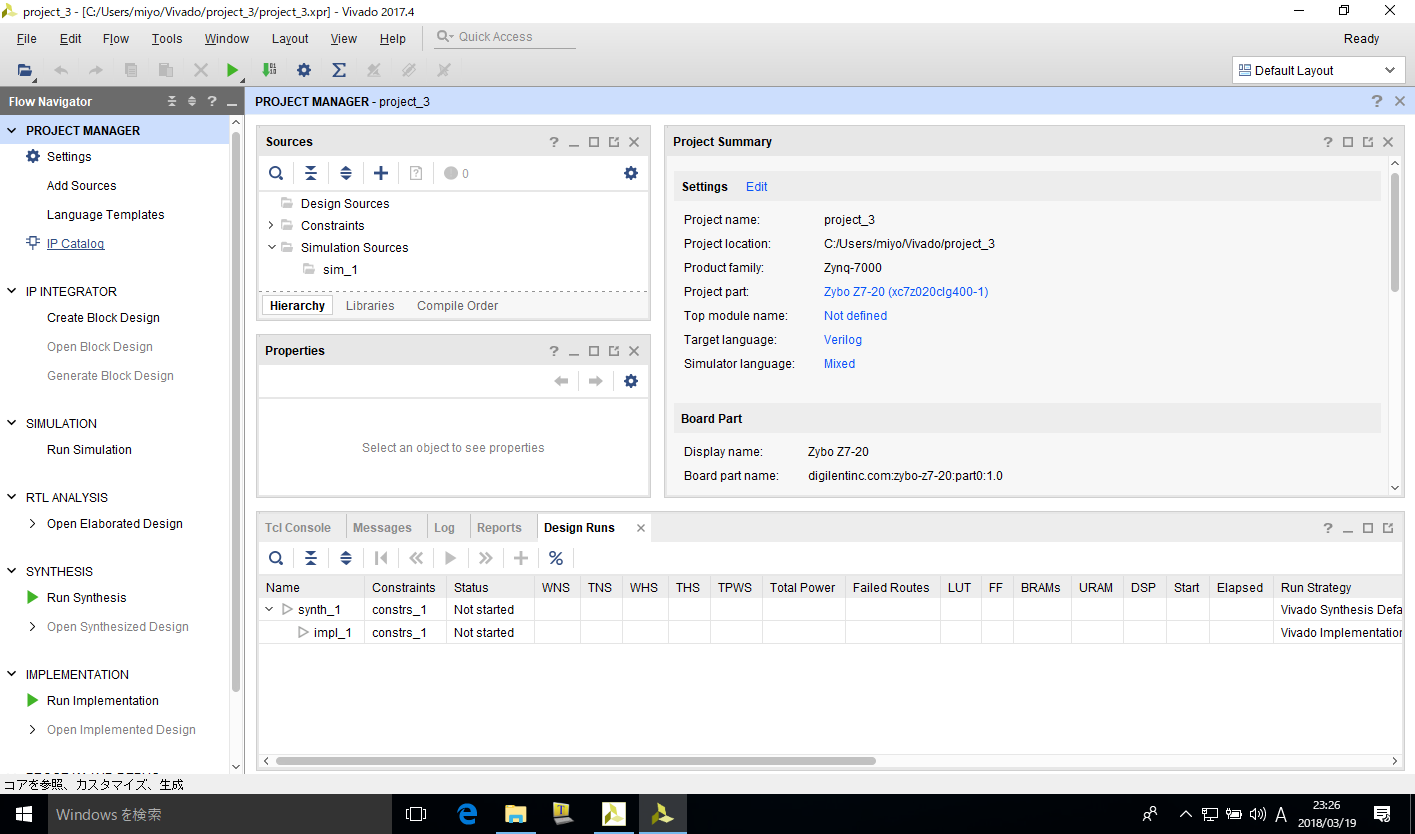
\includegraphics[width=.8\textwidth]{chapter08_figures/VirtualBox_Windows10_19_03_2018_23_26_09.png}
  \end{center}
  \caption{IP Catalogsを選択してIPを呼び出す}
 \end{figure}

 \begin{figure}[H]
  \begin{center}
   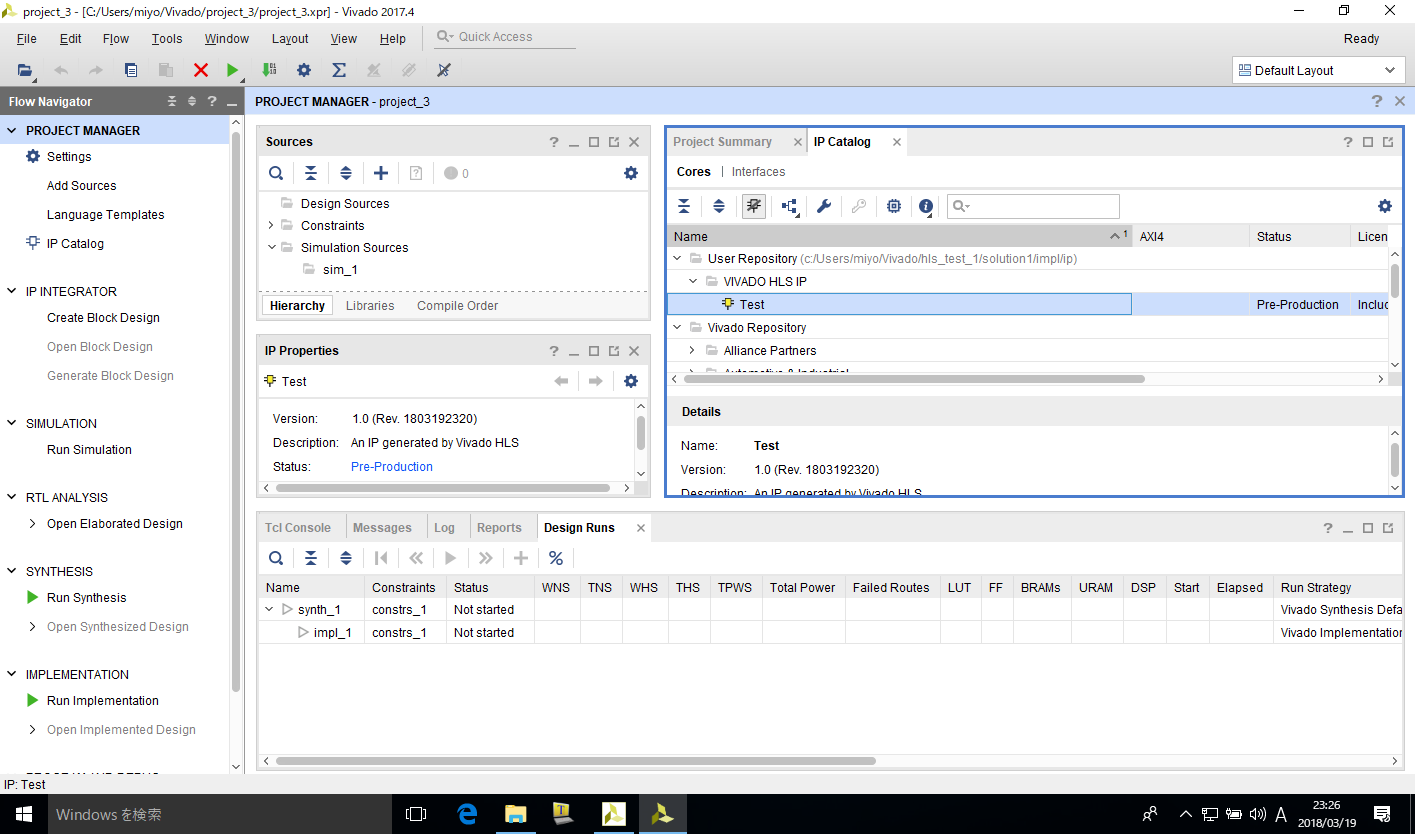
\includegraphics[width=.8\textwidth]{chapter08_figures/VirtualBox_Windows10_19_03_2018_23_26_21.png}
  \end{center}
  \caption{IP Catalogの中にVivado HLSで作成したTestがあるので,ダブルクリックする}
 \end{figure}

 \begin{figure}[H]
  \begin{center}
   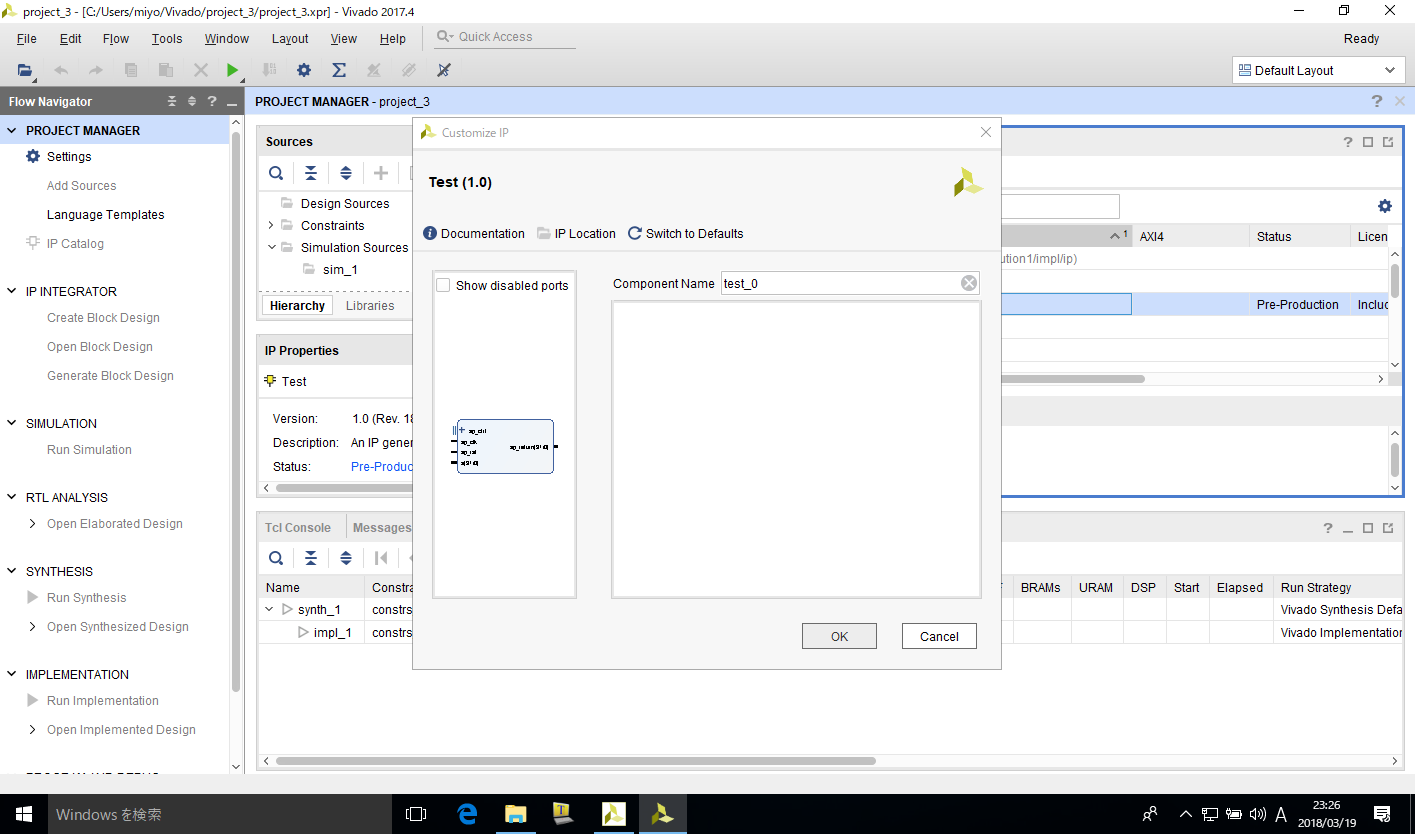
\includegraphics[width=.8\textwidth]{chapter08_figures/VirtualBox_Windows10_19_03_2018_23_26_31.png}
  \end{center}
  \caption{IPコアの設定画面が開くが,することもない.OKを押してダイアログを閉じる}
 \end{figure}

 %%
 \begin{figure}[H]
  \begin{center}
   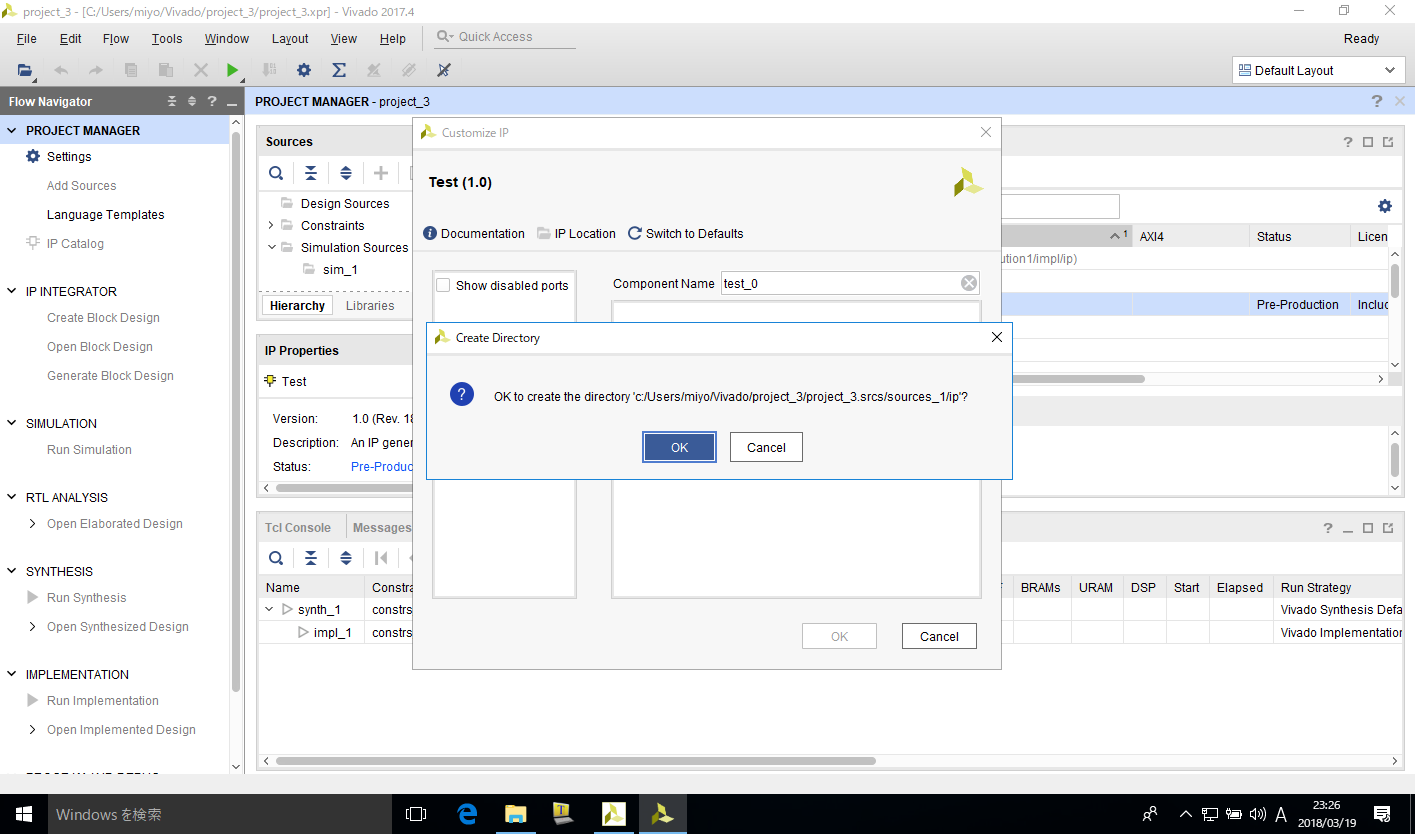
\includegraphics[width=.8\textwidth]{chapter08_figures/VirtualBox_Windows10_19_03_2018_23_26_49.png}
  \end{center}
  \caption{Vivadoプロジェクト内にIPコア保存用のフォルダを作る確認を求められる.OKをクリック}
 \end{figure}

 \begin{figure}[H]
  \begin{center}
   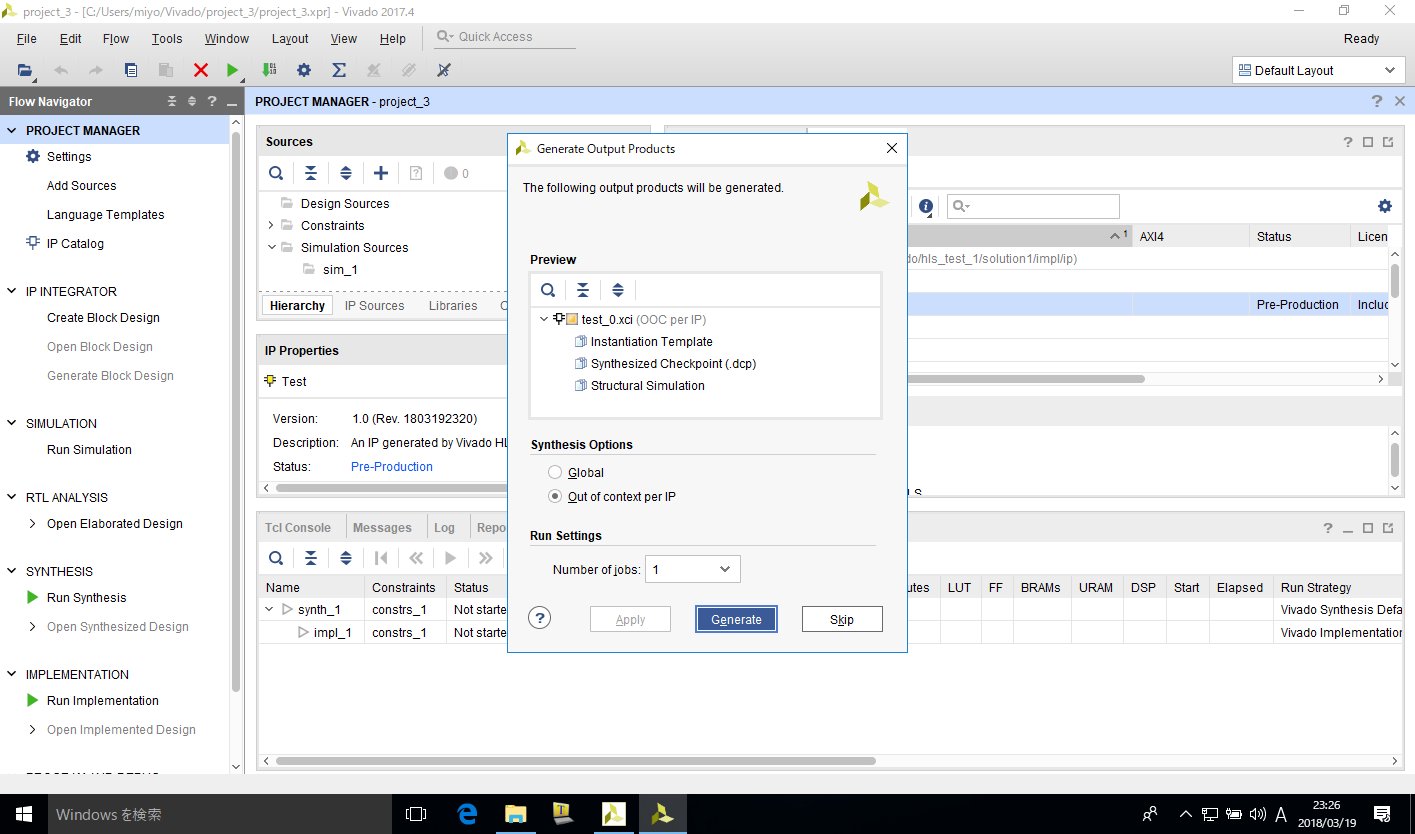
\includegraphics[width=.8\textwidth]{chapter08_figures/VirtualBox_Windows10_19_03_2018_23_26_56.png}
  \end{center}
  \caption{IPコア関連のファイルをVivadoに生成させるためGenerateをクリック}
 \end{figure}

 \begin{figure}[H]
  \begin{center}
   \includegraphics[width=.8\textwidth]{chapter08_figures/VirtualBox_Windows10_19_03_2018_23_27_16.png}
  \end{center}
  \caption{合成がかかる旨のメッセージが表示されたらOKで閉じる}
 \end{figure}

 \begin{figure}[H]
  \begin{center}
   \includegraphics[width=.8\textwidth]{chapter08_figures/VirtualBox_Windows10_19_03_2018_23_27_29.png}
  \end{center}
  \caption{呼びだしたIPコアのインスタンスを持つためのトップモジュールを作成する.モジュールの作成は,Design Sourcesの上で右クリックしてAdd Sources...選択すればよい}
 \end{figure}

 \begin{figure}[H]
  \begin{center}
   \includegraphics[width=.8\textwidth]{chapter08_figures/VirtualBox_Windows10_19_03_2018_23_27_35.png}
  \end{center}
  \caption{今回はデザインファイルを作るので,Add or create design sourcesを選択}
 \end{figure}

 \begin{figure}[H]
  \begin{center}
   \includegraphics[width=.8\textwidth]{chapter08_figures/VirtualBox_Windows10_19_03_2018_23_27_41.png}
  \end{center}
  \caption{Create Fileをクリック.}
 \end{figure}

 \begin{figure}[H]
  \begin{center}
   \includegraphics[width=.8\textwidth]{chapter08_figures/VirtualBox_Windows10_19_03_2018_23_27_50.png}
  \end{center}
  \caption{VHDLで,topという名前のモジュールを作ることにしてOKをクリック.}
 \end{figure}

 \begin{figure}[H]
  \begin{center}
   \includegraphics[width=.8\textwidth]{chapter08_figures/VirtualBox_Windows10_19_03_2018_23_28_00.png}
  \end{center}
  \caption{作成したモジュールがリストに追加されたのでFinishで終了.}
 \end{figure}

 %%
 \begin{figure}[H]
  \begin{center}
   \includegraphics[width=.8\textwidth]{chapter08_figures/VirtualBox_Windows10_19_03_2018_23_33_30.png}
  \end{center}
  \caption{topモジュールの入出力ポートの生成ウィザードが開くので,clkと入出力用のポートを定義してOKをクリックする(あとでテキストで記述してもよいので無視してOKをクリックしても構わない).}
 \end{figure}

 \begin{figure}[H]
  \begin{center}
   \includegraphics[width=.8\textwidth]{chapter08_figures/VirtualBox_Windows10_19_03_2018_23_34_16.png}
  \end{center}
  \caption{生成したトップモジュールをVivadoのエディタで開いたところ}
 \end{figure}

top.vhdの内容は次の内容で書きかえる.
\begin{figure}[H]
\begin{quote}
\begin{Verbatim}[frame=single, numbers=left, baselinestretch=0.8]

library IEEE;
use IEEE.STD_LOGIC_1164.ALL;

entity top is
    Port ( clk : in STD_LOGIC;
           a : in STD_LOGIC_VECTOR (3 downto 0);
           q : out STD_LOGIC_VECTOR (3 downto 0));
end top;

architecture Behavioral of top is

 component test_0
  port (
        ap_clk : in std_logic;
        ap_rst : in std_logic;
        ap_start : in std_logic;
        ap_done : out std_logic;
        ap_idle : out std_logic;
        ap_ready : out std_logic;
        a : in std_logic_vector(31 downto 0);
        ap_return : out std_logic_vector(31 downto 0)
  );
  end component;
  
  attribute mark_debug : string; -- 動作確認のためにmark_debugアトリビュートを使う
  
  signal q_i : std_logic_vector(31 downto 0);
  
begin

 q <= q_i(3 downto 0);

 U : test_0
  port map(
        ap_clk => clk,
        ap_rst => '0',
        ap_start => '1',
        ap_done => ap_done,
        ap_idle => ap_idle,
        ap_ready => ap_ready,
        a(31 downto 4) => (others => '0'),
        a(3 downto 0) => a,
        ap_return => q_i
  );

end Behavioral;
  \end{Verbatim}
 \end{quote}
\end{figure}

 \begin{figure}[H]
  \begin{center}
   \includegraphics[width=.8\textwidth]{chapter08_figures/VirtualBox_Windows10_19_03_2018_23_35_01.png}
  \end{center}
  \caption{コードを正しく記述し終えると,top→test\_0というデザインツリーが作られる}
 \end{figure}

 \begin{figure}[H]
  \begin{center}
   \includegraphics[width=.8\textwidth]{chapter08_figures/VirtualBox_Windows10_19_03_2018_23_35_12.png}
  \end{center}
  \caption{PROJECT NAVIGATORのRun Synthesisをクリックして合成を開始.ダイアログはOKで閉じてステップを進める.}
 \end{figure}

 \begin{figure}[H]
  \begin{center}
   \includegraphics[width=.8\textwidth]{chapter08_figures/VirtualBox_Windows10_19_03_2018_23_36_43.png}
  \end{center}
  \caption{合成を終えたら,一度Open Synthesized Designで合成結果を開く}
 \end{figure}

 \begin{figure}[H]
  \begin{center}
   \includegraphics[width=.8\textwidth]{chapter08_figures/VirtualBox_Windows10_19_03_2018_23_37_20.png}
  \end{center}
  \caption{メニューのLayoutからI/O Planningをクリックしてピン配置設定モードを呼び出す}
 \end{figure}

 \begin{figure}[H]
  \begin{center}
   \includegraphics[width=.8\textwidth]{chapter08_figures/VirtualBox_Windows10_19_03_2018_23_39_38.png}
  \end{center}
  \caption{クロック(K17),入力4bit(T16,W13,P15,G15),出力4bit(D18,G14,M15,M14)を設定.電圧は,すべてLVCMOS33に設定.}
 \end{figure}

 \begin{figure}[H]
  \begin{center}
   \includegraphics[width=.8\textwidth]{chapter08_figures/VirtualBox_Windows10_19_03_2018_23_39_45.png}
  \end{center}
  \caption{設定を終えたらGenerate Bitstreamをクリック}
 \end{figure}

 \begin{figure}[H]
  \begin{center}
   \includegraphics[width=.8\textwidth]{chapter08_figures/VirtualBox_Windows10_19_03_2018_23_39_50.png}
  \end{center}
  \caption{設定したピン配置を保存していいか聞いてくるので,Saveで保存}
 \end{figure}

 %%
 \begin{figure}[H]
  \begin{center}
   \includegraphics[width=.8\textwidth]{chapter08_figures/VirtualBox_Windows10_19_03_2018_23_39_55.png}
  \end{center}
  \caption{設定の保存でSynthesisが無効になる可能性があるという案内がでたら.OKでステップを進める}
 \end{figure}

 \begin{figure}[H]
  \begin{center}
   \includegraphics[width=.8\textwidth]{chapter08_figures/VirtualBox_Windows10_19_03_2018_23_40_00.png}
  \end{center}
  \caption{制約保存用のファイルがないので作成ダイアログに従って作成.名前をtopとしてOKをクリックして完了}
 \end{figure}

 \begin{figure}[H]
  \begin{center}
   \includegraphics[width=.8\textwidth]{chapter08_figures/VirtualBox_Windows10_19_03_2018_23_40_06.png}
  \end{center}
  \caption{Synthesisからやりなおすことの許可を求められるのでYesでステップをすすめる}
 \end{figure}

 \begin{figure}[H]
  \begin{center}
   \includegraphics[width=.8\textwidth]{chapter08_figures/VirtualBox_Windows10_19_03_2018_23_40_11.png}
  \end{center}
  \caption{合成の開始.パラメタはそのままでOKで次へ.}
 \end{figure}

 \begin{figure}[H]
  \begin{center}
   \includegraphics[width=.8\textwidth]{chapter08_figures/VirtualBox_Windows10_19_03_2018_23_45_09.png}
  \end{center}
  \caption{しばらく待つと合成,配置配線が完了してFPGA用のビットストリームが生成される.Open Hardware Managerを選択してOKをクリック.}
 \end{figure}

 \begin{figure}[H]
  \begin{center}
   \includegraphics[width=.8\textwidth]{chapter08_figures/VirtualBox_Windows10_19_03_2018_23_45_17.png}
  \end{center}
  \caption{Hardware Managerが開いたところ.Open targetをクリック.}
 \end{figure}

 \begin{figure}[H]
  \begin{center}
   \includegraphics[width=.8\textwidth]{chapter08_figures/VirtualBox_Windows10_19_03_2018_23_45_23.png}
  \end{center}
  \caption{Auto ConnectでFPGAボードと接続する}
 \end{figure}

 \begin{figure}[H]
  \begin{center}
   \includegraphics[width=.8\textwidth]{chapter08_figures/VirtualBox_Windows10_19_03_2018_23_45_56.png}
  \end{center}
  \caption{Program deviceで生成したbitファイルをFPGAに書き込む}
 \end{figure}


 \subsection{実機で動作を確認}

実機での動作を確認できます.DIPスイッチをON/OFFしたときにONの個数がカウントできていることがわかります.が,残念ながらよくみてみると,DIPスイッチを2つONにした状態,つまり1bit目のLEDのみが点灯すべきケースで,0bit目のLEDが若干点灯していることがわかります.これはバグなので原因を探してみましょう.
 \begin{figure}[H]
  \begin{center}
   \includegraphics[width=.8\textwidth]{chapter08_figures/IMG_0011.JPG}
  \end{center}
  \caption{LEDが一つだけ点灯するはずが0bit目のLEDが若干明るい}
 \end{figure}

ここでは,ILAを使って,実機で動作を確認してみます.まず,topモジュールを次のように書き変えて,いくつかの信号をILAで観測できるようにしましょう.

\begin{figure}[H]
\begin{quote}
\begin{Verbatim}[frame=single, numbers=left, baselinestretch=0.8]

library IEEE;
use IEEE.STD_LOGIC_1164.ALL;

entity top is
    Port ( clk : in STD_LOGIC;
           a : in STD_LOGIC_VECTOR (3 downto 0);
           q : out STD_LOGIC_VECTOR (3 downto 0));
end top;

architecture Behavioral of top is

 component test_0
  port (
        ap_clk : in std_logic;
        ap_rst : in std_logic;
        ap_start : in std_logic;
        ap_done : out std_logic;
        ap_idle : out std_logic;
        ap_ready : out std_logic;
        a : in std_logic_vector(31 downto 0);
        ap_return : out std_logic_vector(31 downto 0)
  );
  end component;
  
  attribute mark_debug : string; -- 動作確認のためにmark_debugアトリビュートを使う
  
  signal q_i : std_logic_vector(31 downto 0);
  attribute mark_debug of q_i : signal is "true"; -- mark_debugに指定
  
  -- ステータス信号を引出しILAで観測するために追加
  signal ap_done : std_logic;  
  signal ap_idle : std_logic;
  signal ap_ready : std_logic;
  attribute mark_debug of ap_done : signal is "true";
  attribute mark_debug of ap_idle : signal is "true";
  attribute mark_debug of ap_ready : signal is "true";
  -- ステータス信号を引出しILAで観測するために追加,ここまで
  
begin

 q <= q_i(3 downto 0);

 U : test_0
  \end{Verbatim}
 \end{quote}
\end{figure}
次のページに続く
\begin{figure}[H]
\begin{quote}
\begin{Verbatim}[frame=single, numbers=left, baselinestretch=0.8]
  port map(
        ap_clk => clk,
        ap_rst => '0',
        ap_start => '1',
        ap_done => ap_done,
        ap_idle => ap_idle,
        ap_ready => ap_ready,
        a(31 downto 4) => (others => '0'),
        a(3 downto 0) => a,
        ap_return => q_i
  );

end Behavioral;
  \end{Verbatim}
 \end{quote}
\end{figure}

 \begin{figure}[H]
  \begin{center}
   \includegraphics[width=.8\textwidth]{chapter08_figures/VirtualBox_Windows10_19_03_2018_23_52_03.png}
  \end{center}
  \caption{コードを書き変えたらRun Synthesisをクリックして合成を行なう}
 \end{figure}

 \begin{figure}[H]
  \begin{center}
   \includegraphics[width=.8\textwidth]{chapter08_figures/VirtualBox_Windows10_19_03_2018_23_55_12.png}
  \end{center}
  \caption{合成がおわったらOpen Synthesized Designで合成結果を開く}
 \end{figure}

 \begin{figure}[H]
  \begin{center}
   \includegraphics[width=.8\textwidth]{chapter08_figures/VirtualBox_Windows10_19_03_2018_23_55_41.png}
  \end{center}
  \caption{ILAの設定をしたいので,メニューのLayoutからDebugを選択}
 \end{figure}

 \begin{figure}[H]
  \begin{center}
   \includegraphics[width=.8\textwidth]{chapter08_figures/VirtualBox_Windows10_19_03_2018_23_55_50.png}
  \end{center}
  \caption{虫のアイコンをクリックしてILA設定ウィザードを開く}
 \end{figure}

 \begin{figure}[H]
  \begin{center}
   \includegraphics[width=.8\textwidth]{chapter08_figures/VirtualBox_Windows10_19_03_2018_23_55_56.png}
  \end{center}
  \caption{ILA設定ウィザードの開始}
 \end{figure}

 \begin{figure}[H]
  \begin{center}
   \includegraphics[width=.8\textwidth]{chapter08_figures/VirtualBox_Windows10_19_03_2018_23_56_09.png}
  \end{center}
  \caption{観測したい信号のクロックをみつけることができずundefinedになっている}
 \end{figure}

 \begin{figure}[H]
  \begin{center}
   \includegraphics[width=.8\textwidth]{chapter08_figures/VirtualBox_Windows10_19_03_2018_23_56_17.png}
  \end{center}
  \caption{クロックを設定したいアイテムの上で右クリックしてSelect Clock Domeinを選ぶ}
 \end{figure}

 \begin{figure}[H]
  \begin{center}
   \includegraphics[width=.8\textwidth]{chapter08_figures/VirtualBox_Windows10_19_03_2018_23_56_29.png}
  \end{center}
  \caption{Global\_CLOCKがないという案内が表示されるがOKで閉じる}
 \end{figure}

 \begin{figure}[H]
  \begin{center}
   \includegraphics[width=.8\textwidth]{chapter08_figures/VirtualBox_Windows10_19_03_2018_23_56_30.png}
  \end{center}
  \caption{Global\_CLOCKのかわりにALL\_CLOCKを選択するとclk\_IBUFが見つかるので選択,OKをクリックする}
 \end{figure}

 \begin{figure}[H]
  \begin{center}
   \includegraphics[width=.8\textwidth]{chapter08_figures/VirtualBox_Windows10_19_03_2018_23_56_44.png}
  \end{center}
  \caption{同様の手順で全ての信号のClock Domainをclk\_IBUFに設定したらNextで次へ}
 \end{figure}

 %%
 \begin{figure}[H]
  \begin{center}
   \includegraphics[width=.8\textwidth]{chapter08_figures/VirtualBox_Windows10_19_03_2018_23_56_52.png}
  \end{center}
  \caption{サンプル数や利用機能はデフォルトのままでよいのでNextで次へ}
 \end{figure}

 \begin{figure}[H]
  \begin{center}
   \includegraphics[width=.8\textwidth]{chapter08_figures/VirtualBox_Windows10_19_03_2018_23_58_59.png}
  \end{center}
  \caption{サマリを確認したらFinishでウィザードを閉じる}
 \end{figure}

 \begin{figure}[H]
  \begin{center}
   \includegraphics[width=.8\textwidth]{chapter08_figures/VirtualBox_Windows10_19_03_2018_23_59_22.png}
  \end{center}
  \caption{ILAの挿入ができたので,あらためてGenerate Bitstreamで合成と配置配線を行なう}
 \end{figure}

 \begin{figure}[H]
  \begin{center}
   \includegraphics[width=.8\textwidth]{chapter08_figures/VirtualBox_Windows10_19_03_2018_23_59_29.png}
  \end{center}
  \caption{ILAに関する設定を保存するか確認を求められたらSaveをクリック}
 \end{figure}

 \begin{figure}[H]
  \begin{center}
   \includegraphics[width=.8\textwidth]{chapter08_figures/VirtualBox_Windows10_20_03_2018_00_20_08.png}
  \end{center}
  \caption{しばらく待つとILAを仕込んだビットストリームが生成される.Open Hardware Managerを選択してOKをクリック}
 \end{figure}

 \begin{figure}[H]
  \begin{center}
   \includegraphics[width=.8\textwidth]{chapter08_figures/VirtualBox_Windows10_20_03_2018_00_20_15.png}
  \end{center}
  \caption{新しく作ったビットストリームを書き込むためにProgram Deviceをクリック}
 \end{figure}

 \begin{figure}[H]
  \begin{center}
   \includegraphics[width=.8\textwidth]{chapter08_figures/VirtualBox_Windows10_20_03_2018_00_20_20.png}
  \end{center}
  \caption{ビットストリームとILA用の定義ファイルがセットされていることを確認してProgramをクリック}
 \end{figure}

 %%
 \begin{figure}[H]
  \begin{center}
   \includegraphics[width=.8\textwidth]{chapter08_figures/VirtualBox_Windows10_20_03_2018_00_20_58.png}
  \end{center}
  \caption{二重三角マークをクリックすると内部信号が確認できる}
 \end{figure}

 \begin{figure}[H]
  \begin{center}
   \includegraphics[width=.8\textwidth]{chapter08_figures/VirtualBox_Windows10_20_03_2018_00_22_19.png}
  \end{center}
  \caption{ap\_doneが'1'でない間に値がふらふらしていることが確認できた.}
 \end{figure}

 \subsection{Vivado HLSのシミュレーション結果を詳細に確認する}

実はILAを挿入するまでもなく,Vivado HLSのC/RTL協調シミュレーションの結果を注意深く確認することで,今回のバグは防ぐことができます.試してみましょう.

 \begin{figure}[H]
  \begin{center}
   \includegraphics[width=.8\textwidth]{chapter08_figures/VirtualBox_Windows10_20_03_2018_00_23_02.png}
  \end{center}
  \caption{Vivado HLSでC/RTLシミュレーションを再度実行する}
 \end{figure}

 \begin{figure}[H]
  \begin{center}
   \includegraphics[width=.8\textwidth]{chapter08_figures/VirtualBox_Windows10_20_03_2018_00_23_15.png}
  \end{center}
  \caption{シミュレーション実行パラメタのDump Traceでallを選択してOKをクリック}
 \end{figure}

 \begin{figure}[H]
  \begin{center}
   \includegraphics[width=.8\textwidth]{chapter08_figures/VirtualBox_Windows10_20_03_2018_00_27_29.png}
  \end{center}
  \caption{シミュレーションが完了すると,ツールバーのOpen Wave Viewerをクリックする}
 \end{figure}

 \begin{figure}[H]
  \begin{center}
   \includegraphics[width=.8\textwidth]{chapter08_figures/VirtualBox_Windows10_20_03_2018_00_30_04.png}
  \end{center}
  \caption{しばらく待つとVivadoシミュレータの波形ビューワが開く.ここでC/RTLシミュレータの結果を確認できる.}
 \end{figure}

 \begin{figure}[H]
  \begin{center}
   \includegraphics[width=.8\textwidth]{chapter08_figures/VirtualBox_Windows10_20_03_2018_00_31_28.png}
  \end{center}
  \caption{結果の信号やap\_doneなどを波形ビューワに追加してみたところ.ap\_doneが'1'でない場合に値が確定していないため注意しなければならない,ということがみてとれる.}
 \end{figure}

 \subsection{再度実機での動作確認}
バグ修正を反映して,もう一度,実機で動作を確認してみましょう.

\begin{figure}[H]
\begin{quote}
\begin{Verbatim}[frame=single, numbers=left, baselinestretch=0.8]

library IEEE;
use IEEE.STD_LOGIC_1164.ALL;

entity top is
    Port ( clk : in STD_LOGIC;
           a : in STD_LOGIC_VECTOR (3 downto 0);
           q : out STD_LOGIC_VECTOR (3 downto 0));
end top;

architecture Behavioral of top is

 component test_0
  port (
        ap_clk : in std_logic;
        ap_rst : in std_logic;
        ap_start : in std_logic;
        ap_done : out std_logic;
        ap_idle : out std_logic;
        ap_ready : out std_logic;
        a : in std_logic_vector(31 downto 0);
        ap_return : out std_logic_vector(31 downto 0)
  );
  end component;
  
  attribute mark_debug : string;
  
  signal q_i : std_logic_vector(31 downto 0);
  attribute mark_debug of q_i : signal is "true";
  
  signal ap_done : std_logic;
  signal ap_idle : std_logic;
  signal ap_ready : std_logic;
  attribute mark_debug of ap_done : signal is "true";
  attribute mark_debug of ap_idle : signal is "true";
  attribute mark_debug of ap_ready : signal is "true";
  
begin
 -- バグ修正のために追加
 process(clk)
 begin
   if rising_edge(clk) then
     if ap_done = '1' then
       q <= q_i(3 downto 0);
     end if;
  \end{Verbatim}
 \end{quote}
\end{figure}
次のページに続く
\begin{figure}[H]
\begin{quote}
\begin{Verbatim}[frame=single, numbers=left, baselinestretch=0.8]
   end if;
 end process;
 -- バグ修正のために追加,ここまで

 U : test_0
  port map(
        ap_clk => clk,
        ap_rst => '0',
        ap_start => '1',
        ap_done => ap_done,
        ap_idle => ap_idle,
        ap_ready => ap_ready,
        a(31 downto 4) => (others => '0'),
        a(3 downto 0) => a,
        ap_return => q_i
  );

end Behavioral;
  \end{Verbatim}
 \end{quote}
\end{figure}

 \begin{figure}[H]
  \begin{center}
   \includegraphics[width=.8\textwidth]{chapter08_figures/VirtualBox_Windows10_20_03_2018_00_32_36.png}
  \end{center}
  \caption{コードを書き変えたらGenerate Bitstreamをクリックして,再度ビットストリームを生成する}
 \end{figure}

 \begin{figure}[H]
  \begin{center}
   \includegraphics[width=.8\textwidth]{chapter08_figures/IMG_0015.JPG}
  \end{center}
  \caption{再び実機で動作を確認したところ.LEDが正しく一つだけ点灯していることがわかる.}
 \end{figure}


\end{document}
